\begin{abstract}
The rapidly growing interest in autonomous driving has gathered a lot of research efforts in this area over the last decade. Many manufacturers, and other tech companies have started testing of prototype vehicles in controlled environments. However, implications of a large amount of autonomous fleet presents new research challenges. To handle dynamic environments, the car requires accurate and updated information about its surrounding. To provide safety and comfort to the passengers, a high-definition map is needed to complement an autonomous car's on-board sensors for such information. It is a centimeter-accurate virtual representation of the real world. A high-definition map allows an autonomous car to localize itself precisely and navigate itself in a highly dynamic environment of the real world. Such an accurate representation of the world is also subjected to change very often. Thereby, requiring constant update from a remote server for the map. This thesis investigates this issue to provide a method to enable a constant stream of updates to a navigation system. The main contribution of this thesis is a method that finds contextually relevant map data for minimizing update size. The proposed method ensures safe and comfortable driving while keeping the necessary data bandwidth and processing time as low as possible. The method's capability has been evaluated on the map databases of the German city of Berlin. The obtained results indicate that the proposed solution saves significant amounts of data and processing time compared to existing map update solutions.
\end{abstract}



%*****************************************
\chapter{Introduction} \label{ch:introduction}
%*****************************************
\section{Motivation} \label{motivation}
Car navigation started as a feature of luxury cars in 1980s \cite{schaminee2011short}. However, the initial growth of such systems was limited by the sales of expensive luxury cars. Moreover, it was a very primitive system without any Global Positioning System (GPS). Many factors such as the exponential growth in automobile industry and the availability of GPS signal for civilian use have led to the perception of navigation systems as an essential feature of our cars today. One of the most popular early versions of such navigation systems was by \citet{ishikawa1991map}. The growing need to innovate at a faster rate provided space for new companies to focus on navigation solutions and innovate in that area. This has led to many successful companies such as TomTom, Garmin, HERE etc. which have pioneered in the area of personal navigation systems.\\

Autonomously driving cars or simply autonomous cars have been a topic of interest for the last century. Although, very little progress was made in terms of an actual product, there were many small research projects in every decade which made some contribution to this field. These projects were often demonstrated at trade fairs to show a company's technological advancement. However, the research in the area of autonomous driving started to gain ground only after the 1980s. Viability of cars that could steer themselves in complex urban environments such as streets and highways were demonstrated only after 1980s. Advancements in sensing technologies and computation power helped fuel the research in autonomous vehicles. Challenges like Defense Advanced Research Project Agency (DARPA) Grand Challenge also helped in gaining attention in this research field. \citet{dickmanns2002development}, \citet{thorpe1991toward} and many contestant teams of the DARPA Grand Challenge (DGC) have showcased their work of building complex systems to achieve this goal. \citet{campbell2010autonomous} have summarized the different approaches used by different research groups to solve these complex problems. Their paper also discusses the challenges which are yet to be conquered. One of such challenges is autonomous vehicles in dynamic environments such as urban areas. While testing of fully autonomous vehicles has been rolled out by some companies, it is still in tightly controlled test environments or limited areas. \\

Various approaches described by Campbell et al. to solve complex navigation problems in autonomous cars involve sensor based inputs. More recent approaches described by \citet{levinson2011towards} in their paper discusses the use of light detection and ranging (LIDAR) systems combined with a variety of sensors on the car. Such approaches are targeted more towards solving dynamic object detection, which suits the urban environment. Many automobile companies have begun testing their prototype vehicles in controlled environments. However, a dynamic environment presents new challenges to autonomous driving. Based on a study by \citet{aeberhard2015experience}, autonomous cars in 2016 cannot completely rely on on-board sensors for navigation. A high-definition map, however presents a promising solution \cite{360hdmaps}, \cite{hdmapauto}). A high-definition map (HD-map) is a centimeter accurate virtual representation of the real world. It provides much more accurate details of roads and lanes for an autonomous car to navigate in a dynamic environment. When used in combination with other on-board sensors of an autonomous car, it will ensure the safety and comfort of the passengers and other road users. A high-definition map allows a car to see and understand what it cannot with the help of on-board sensors. For instance, the detection range of a modern sensor based autonomous vehicle is limited to 200 meters in an ideal condition. Weather conditions such as rain or snowfall, improper light conditions and bad sign-boards could reduce that range further as these conditions are a source of potential sensor inaccuracy and false detection events. A high-definition map will compensate for such sensor insufficiency. Companies like Waymo, formerly known as Google self-driving project (\citet{madrigal}), HERE (\citet{stevenson}), TomTom (\cite{tomtom}) and car manufacturers like BMW (\citet{bender2014lanelets}, \citet{aeberhard2015experience}) and Tesla (\citet{perkins}) rely on such high-definition street maps for their own highly automated vehicle systems. \\


The high-definition maps are extremely detailed; therefore they require much more storage space when compared to the conventional map data. Thereby, making it largely impossible to store a complete detailed map in a navigation system. Moreover, these high-definition maps tend to change more often as they reflect on the data collected by autonomous vehicles as sensory nodes. For an autonomous car to navigate safely and to ensure the comfort and safety of the passenger, these high-definition maps require a constant stream of updates. Any information relevant to the car should be provided to it in advance through the representation as a map object. This could be for example detailed information about construction sites, the current status of variable traffic signs, areas of accidents, traffic jams or dangerous weather conditions like ice and snow. In this way the high definition street map changes its purpose from sole road guidance to a severe feature to ensure safety and comfort for the passengers inside the car. Dynamic events like the occurrence of a traffic accident have to be transferred immediately. \\ 
 
Online navigation systems use the computing power of a large cluster of computers to deliver the optimal route along with required map data over an internet connection. Receiving such a large amount of map data over a cellular connection is very expensive, especially if the autonomous car is in a roaming network. Moreover, an online navigation systems does not function without a cellular connection. Therefore, an online navigation system is not practical for an autonomous car because of the high operational costs of map data and the rigid requirement of a cellular connection. On the other hand, offline navigation systems can work without a cellular connection. To store such large amount of information and to allow faster routing queries, a binary file based format is used in navigation system. However, such formats render devices incapable of introducing map updates as stated by \citet{min2008mobile}. However, if such a navigation system is never updated, its routing performance will deteriorate over time since the road networks and other factors such as traffic change quite often. \\

It is clear that the high-definition maps are a necessary for the autonomous cars to drive in dynamic environments. To reduce operational costs of a cellular data connection, we investigate the problem of minimizing update sizes for such high-definition maps. We present our approach along with a protocol which can reduce the size of map updates depending on the context. \\

\section{Scope} \label{scope}
As stated in the motivation, we are only considering navigation devices which rely on offline navigation data for processing a user's navigation request. Ordinarily, we are assuming that, such a navigation device has cellular connectivity in order to receive map updates. The evaluation of our approach does not involve comparison with an online navigation system. There can be several functions provided by the map data. We are only considering navigation functions built upon the map data and consequently navigation requests in this work. Accordingly, the map updates referred to in this work are related to navigation functions only.

\section{Outline}
This thesis is organized in the following manner. Chapter \ref{ch:background} describes the necessary information required for understanding different navigation systems and the basics of digital maps. In Chapter \ref{ch:relatedwork}, state-of-the-art related work by other researchers has been covered. We also discuss their significance and their contribution to our idea in the same chapter. In Chapter \ref{ch:approach}, we present our novel concept of utilizing relevance of a map data to a navigation request. We also present a Dynamic Map Update Protocol based on our concept in the chapter. After explaining our concept, we discuss our implementation in Chapter \ref{ch:implementation}. The evaluation of our approach is explained in Chapter \ref{ch:evaluation}, which includes the evaluation setup and the different scenarios we have developed. We also discuss the significance of the results. In Chapter \ref{ch:conclusion}, we conclude our work with a forward looking approach.


\chapter{Theory} \label{ch:background}
We now explain different types of navigation systems and provide a comparison between them. Later in this chapter, we discuss the existing update processes for such systems as well. We then provide a short introduction to different digital maps concepts and related concepts used in this work. We also discuss in details, an open map format and provide insight into how map data is related, stored and processed.

\section{Available Navigation Systems}
Today many different navigation solutions exist for cars worldwide. Most of them come pre-installed in the car by the manufacturer. These built-in navigation systems are called in-car navigation systems. Such systems are responsible for car navigation system and provide many other services such as emergency assist, on-road assist as well. The map updates to such navigation systems are in-general provided by their respective device manufacturers. \\

Another alternate option for car navigation system is aftermarket solutions by large navigation companies such as TomTom \cite{schafer2009iq}, Garmin \cite{garminauto} etc. Most of the devices manufactured by these companies are compatible with or comes as an accessory to the car's existing infotainment system. These devices are bought separately and the software \& map updates are provided by these navigation companies.

\subsection{Offline Navigation Systems} \label{offlinenav}
We explained different types of navigaiton systems that are available today. We now discuss the offline navigation systems and discuss their features. Most of the factory installed navigation systems and aftermarket solutions by third parties can be classified as offline navigation systems. These systems have no or limited internet connectivity. Such systems rely on a digital map pre-installed on the device to provide navigation functions. While the map installed in such systems could be out-dated, some systems such as Toyota \citep{ishikawa1991map} provide an additionally functionality to provide traffic \& other incident information via Radio Data System (RDS) or other standards. Often, these features came with an additional subscription fees. Over the last two decades navigation systems in cars have evolved. While vehicle manufacturers focused largely on advancing complex automotive technologies, the pace of innovation for in-car navigation systems was relatively slow \cite{schaminee2011short}. This created an opportunity for new players to invest more in car navigation system than the typical car original equipment manufacturer (OEM). Many electronics, digital mapping companies were formed to work on advancing mapping and navigation systems for cars. They offered their solutions directly to car manufacturers, as well as consumers. Such developments have led to much advancement in this field. In the early days of navigation system, it was offered as a feature of luxury cars line, nowadays it has become an essential feature of a modern day car. This field is no longer dominated by car manufacturers but smart digital mapping companies like TomTom, Garmin, HERE Maps which have developed their own digital mapping solutions to solve various problems related to navigation systems in cars.\\

An offline navigation system is a navigation system which does not have any connectivity to the internet or a remote server. Such a system relies on locally stored map data to provide navigation services to the user. The map data could be stored on built-in storage in such system or an external storage such as SD card or USB memory stick. All the navigation services are offered based on the map data available. Depending upon the service provider and data available, multiple services such as live traffic information, points of interest (POI) locator could be available. For a navigation query, the system would find shortest/optimal path to the destination using the map data. As pointed out by Ling \cite{navinfo} who is President of NavInfo (\textit{China's leading provider of digital maps and telematics}), map updates are crucial for maintaining optimum performance of a navigation system. Ling argues that if not updated, the performance of a navigation system will deteriorate as new streets and other points of interests (POI) are being added/updated daily in their maps. The amount of changes produced in conventional maps are relatively larger for growing economies like China, India and other emerging countries. \\

The map update process (Section \ref{existingUpdate}) of offline navigation systems is designed by the device manufacturers. Updating the map data of such devices requires map updates from their respective device manufacturers or map data providers. The device manufacturers have to extensively test the map updates for their devices to avoid any bugs and provide the updated map information in their proprietary format. Such comprehensive processes add delay and hence the updates are released in different cycles. Hence, these devices are incapable of responding to the quick changes in a real world as they have to wait for the manufacturers to release an update. Another factor limiting this is that the map updates are sold as part of subscriptions and/or new purchases by the customers. To retain customers, manufacturers use proprietary format and have to provide value in the purchase of the update. These factors combined make the offline navigation systems in its current form, not a suitable choice for an up-to-date navigation system for an autonomous car. \\

We briefly explained the features of offline navigation systems and highlighted their suitability to be used in an autonomous vehicle. We now discuss two companies, Garmin \& TomTom, which are famous for providing such offline navigation systems.   
 
\subsubsection{Garmin}
Garmin Ltd. is one of the leaders in navigation systems. They are relatively new to the automotive navigation sector. However, they have one of the largest market share when it comes to after-market navigation systems. Garmin started offering automotive navigation solutions only after 1998 and offered pre-installed maps of the region in a flash storage within the device. The maps were pre-installed and newer versions supported traffic notifications via Radio Data Standard (RDS). Garmin relied on maps data from Navteq (which is now part of HERE), it pioneered in hand-held small Global Positioning System (GPS) used in the navigation system and other devices. Garmin uses in-memory vector-based maps to provide faster navigation results and stores additional data in additional flash storage. Garmin periodically offers detailed updated maps for purchase.
\subsubsection{TomTom}
TomTom is well known for its aftermarket navigation systems. Through initial years since its incorporation in 1990s, it was mostly focused on business to business solutions. The promising growth in automobile sector and the market for aftermarket devices for cars pushed many companies to provide their navigation solutions. TomTom was one of the first companies to launch an aftermarket portable navigation device (PND) for consumers \cite{tomtomhistory}. This category of device has witnessed tremendous growth in the last decade. Through acquisitions and partnerships with companies, TomTom maps are part of many innovative navigation solutions, both offline and online. To improve navigation results, TomTom integrated traffic data in its products using a cellular connection. 


\subsection{Online Navigation Systems}
Earlier in this chapter, we looked at offline navigation systems and covered their features. We now discuss their counterpart, the online navigation systems and explain their differences. Over the last two decades, we have witnessed an exponential growth in the use of mobile phones. With such a growth in consumer devices with connectivity, access to information and digital media has grown rapidly as well. According to report by \citet{gantz2012digital} the amount of data used by consumers will witness a 50-fold growth in current decade. While navigation services being one of the most popular service of mobile devices, it is required that the cost of using such services should remain low. The offline navigation systems provide navigation services without typical operational cost. However, their performance deteriorates over time and the complex map update procedure costs both in terms of money and time. Such disadvantages of the offline navigation systems (Section \ref{offlinenav}) are non-existent in their online counterparts. The online navigation systems are devices with cellular connectivity. Storage of map data is not typically required in an online navigation system. Such a system is mainly designed to act as an interface to a large cluster of highly capable systems or a cloud. The central map server keeps itself updated by acquiring information such as traffic information, incident information such as construction works or even accidents from various public sources such as government and private sources such as traffic monitoring companies. Such information is used to find the best possible route for navigation requests sent to the central map server by many such online navigation systems. \\

Almost all of the online navigation systems work typically in a similar fashion. They take user input such as destination in form of an address or places/categories of interest along with user's or vehicle's current location. Using the navigation device's cellular connection, it passes these information to the central server for processing. Using the vehicle's location and query parameters it received along with the updated map information, the central server replies back with a response in a format the device can understand. Such a response may include direction steps to the destination user requested or nearby restaurants to be shown on the map. 
We will now explain in brief, two of the most prominent standards that are available today for using an online navigation system in a car. Such online systems are quite popular navigation choices among users as it does not require a separate device to be purchased. However, these systems are not designed for autonomous cars as the amount of data required for high-definition maps for autonomous cars is too high. However, we would still cover some details about them and try to show their downsides. 

\subsubsection{Apple CarPlay}
The Apple iPhone is one of the most popular devices in the world today. With CarPlay \cite{AppleCarPlay}, Apple introduced CarPlay as a standard to control the in-car navigation/infotainment system using the iPhone. Most worldwide vehicle manufacturers have incorporated or will be incorporating Apple CarPlay into their in-car system. The availability of Apple CarPlay is limited to select cars, however it is gaining popularity rapidly. A recent disclosure by Apple \cite{Carplaymodels} pointed this figure to be more than 200 different models of cars. \\

The principal objective of Apple CarPlay is to offer a distraction free, seamless environment in car using iPhone's functions in a car's dashboard. For navigation feature, it uses Apple Maps \cite{AppleMaps} from the iPhone. The iPhone's GPS is used to localize the vehicle and cellular connection is used to provide data connection for fulfilling navigation requests. While Apple Maps offer an extensive amount of details and point of interest, most of the calculations are done in the cloud servers. The car's dashboard serves as a display for map services offered by Apple Maps. The current state of Apple Maps supports storing some navigation data offline. However, the operations are limited as the offline mode does not provide any navigation service, only rendering of map is supported in the offline mode. A strong data connection is required for maps to function correctly. As discussed previously, while online maps offer current updated maps, their functioning is completely dependent on cellular data connection. Without a strong data connection, their use as a navigation system is unsupported. 

\subsubsection{Android Auto}
While Android being the most popular mobile operating system, Google's answer to Apple CarPlay is called Android Auto \cite{AndroidAuto}. It is available as a standalone app in Google's app store, popularly known as Google PlayStore \cite{playstore}. Android Auto is backed by Open Automotive Alliance \cite{oaa} which is comprised of car manufacturers, software companies, semiconductor companies and even electronics manufacturers. The functionality offered by Android Auto is similar to that of Apple CarPlay. While Apple CarPlay is largely restricted in cars offered by manufacturers who are listed as supported on Apple's website \cite{Carplaymodels}, several aftermarket car audio systems by electronics manufacturers support Android Auto. However, the functionality offered by such aftermarket devices is limited. \\

Similar to Apple CarPlay, Android Auto relies on Google Maps \cite{googlemaps} application to service navigation requests. The functionality of Google Maps is quite similar to that of Apple Maps, however they have pioneered the map details collection over last few years. Unlike Apple Maps, Google Maps provides an offline mode which supports navigation queries. However, to keep the map data current, it requires it to be updated every 30 days \cite{maps30expire}. The update process of such offline mode map is similar to that of an offline navigation systems. Although, Google Maps provides certain advantage over Apple Maps, it is still unpractical to be used for autonomous cars due to high bandwidth and large storage space requirements of a high-definition map which we discussed earlier (Chapter \ref{ch:approach}). 

\subsection{Hybrid Navigation Systems / Connected Car}
We previously discussed both offline and online navigation systems and their limitations. We saw that while the online navigation systems provide an up-to-date map data, they rely completely on the internet connection for providing such service. Without an internet connectivity, such online navigation systems would fail to work. On the other hand, an offline navigation system has a very low cost of operation as the required map data is available in its storage. However, the navigation performance of such a system can deteriorate over time as the map data becomes dated. We now present a new class of navigation systems which are not purely offline or online. Such systems use offline storage for map data, however they receive updates via cellular connectivity. Such systems are often associated with subscription services by car manufacturers who also provide other features such as Points of Interest (POI) and traffic updates through the cellular connection. In absence of cellular connectivity, such systems behave like offline navigation systems. For finding optimal route, such systems use traffic information through cellular connectivity to choose one of the suggested routes based on local map data. Such class of navigation devices is capable of receiving and applying map and other software updates as well. Such systems are not only capable of providing navigation services but to enhance the driving experience of the driver. The automobile sector has witnessed tremendous growth in connected cars over the last decade. A study by \citet{swan2015connected} discusses how such systems are enhancing the driving experience and creating new business models and quantifying the complete experience. In his paper, one of the industry analyst firm predicts that 75\% of vehicles sold in 2035 will have some sort kind of autonomous capability. While car manufacturers are racing to create new services through apps and to find new business models for their connected car ecosystems, navigation service would still remain one of the mostly used service. We would now look into some of such hybrid navigation systems.
 
\subsubsection{BMW ConnectedDrive}
BMW ConnectedDrive \cite{bmwcd} system was designed to cut down distractions for the driver, it is an enhanced system for controlling vehicle's entertainment, information, communication and navigation. The navigation system in BMW ConnectedDrive is one of the many examples of hybrid navigation systems. The system was designed to provide various services and apps through the car's on-board computer. Initially, the ConnectedDrive experience was limited in connectivity to only mobile devices. However, in 2014 BMW announced newer functions with cellular connectivity to the vehicle. This uses a SIM based cellular connection for data and voice. While pairing with a smart-phone is supported, the system is designed to work with its own cellular connection in absence of that. BMW provides various driver assistance services through ConnectedDrive such as emergency call system, on-road assistance etc.. However, with the cellular connectivity it has started to provide real-time traffic updates to the on-board navigation system. With the increase in mobile computing power, enhanced safety features are also provided by the car's on-board computer for example warnings for blind-spots.


\subsubsection{GM ONStar}
General Motors (GM) ONStar \cite{barabba2002multimethod} is a subscription based enhanced driver assistance service offered in vehicles produced by GM group. OnStar services include emergency assistance, security services, navigation services and cellular connection services. OnStar uses a SIM based cellular connection for all these services. Similar to BMW's ConnectedDrive, OnStar allows you to access bundle of entertainment, information services via car's on-board computer. For navigation services, OnStar provides Turn-by-Turn directions which can use map data stored locally in the car's navigation system and includes information about traffic from a partner map provider. With smart-phone pairing option, OnStar allows seamless navigation services as destination could be shared by smart-phone to car's on-board computer via bluetooth. Other apps and services are being added by GM to enhance the driving experience of the driver. One of the advanced service offered by OnStar allows drivers to call an OnStar number and tell the destination to receive turn-by-turn directions to the destination over cellular data. However, these turn-by-turn directions are voice based thereby reducing the amount of data to be downloaded. 

\subsection{Update Process for Maps} \label{existingUpdate}
Different types of navigation systems were covered in the previous section. Now, we are going to discuss how they provide map updates. Since online navigation systems completely rely on cellular connection for sending navigation query and receiving directions along with map data. we are going to focus on offline and hybrid navigation systems. The online navigation systems are designed to use a remote server's map data for providing navigation services. However, to save bandwidth, online navigation systems can use cache of previously used map data. However, as discussed in Section \ref{scope}, we would only consider map update processes for offline and hybrid navigation systems. \\

The offline and hybrid navigation systems use proprietary storage format for storage map data. The choice for using a binary data format such as the Physical Storage Format (PSF) is for to reasons like
\begin{enumerate}
\item faster routing based on file-system based indexes
\item less storage space needed.
\end{enumerate}
Despite all these advantages, as discussed by \citet{min2008mobile} in his work, it offers no other advantage when it comes to updating the maps bz using a binary format for storage. The update process of an offline navigation system is limited to data provided through an external data source for the updated map data. The typical approaches include downloading updated map data for a selected region into a computer. Then copying the downloaded data into a USB stick or SD card. And then connecting that USB stick or SD card to the car's navigation system and then choosing process to update. This could sometimes take upto 2 hours \cite{garminupdate}. Another approach for updating map data is by connecting the navigation device to a computer which is connected to internet. By using a software supplied by the device manufacturer, compatible map data could be directly downloaded onto the navigation system. This method provides relatively easier approach, however it is supported typically by aftermarket solutions. For factory installed navigation systems, it is typically done via method involving a USB stick or SD card. The complete storage of binary data has to be overwritten to allow updates. Even for small changes, the whole storage has to be written again. The fact that even for small changes, the whole binary format map data has to recompiled. This limits the Physical Storage Format (PSF) from being an ideal format for constant update process. Additionally, optimization and other pre-processing of the PSF file also contribute in delay of release of updated maps to the users. Thereby, the physical storage format of offline navigation systems hinders users from having the up-to-date map data. 
\\

In summary, because of the binary map format, a vicious cycle of a time consuming update process is formed and thus less frequent map updates are released by the manufacturers. To overcome this, alternative formats for storing the map data have been implemented and are in use today. We have explained some of these formats and described their working in Chapter \ref{ch:relatedwork}. We will now look at some concepts about maps and describe briefly some of the concepts in the next section.


\section{Basic Concepts of Maps}
Maps have been around for centuries now. However, their use was limited to only certain groups. Computer based digital maps became available only after late 1960s as reported by \citet{coppock1991history} in their paper. Coppock and Rhind have described the different approaches involved in the development of Geographic Information Systems or simply GIS. They present the history of digital maps building in their paper and showcase the shift in map generation. Their work discusses three different phases of the digital mapping revolution. The first phase, from the early 1960s to about 1975. The second phase expanding from 1973 until the early 1980s saw many experiments and early uses of GIS in different environments. The third phase, from 1982 until the late 1980s witnessed many commercial applications of previous experiments. The fourth phase, the current phase is witnessing standardizations and user-centric adaptation of digital mapping technologies.\\


For definition, digital mapping could be described as a process of collection of map data to create a virtual image of the world. While the primary function is to produce accurate maps, the digital format allows certain computations on the map data itself. One such example could be the calculation of route between two points on a map. The use of digital maps has exploded in recent years. It has found its applications in many previously known fields such a geography, archeology, urban planning. Digital maps are finding their way in various use cases such as advertising and even augmented reality. Historically, the sources of such digital maps have been government agencies and department with the use of computer scientists, cartographers, remote-sensing satellites. However, in recent years volunteered geographic information projects such as the OpenStreetMap ( Section \ref{osm} ) have seen tremendous participation and has fueled growth in innovative solutions using these open-license digital maps. 
\subsection{Geographic Coordinate System}
To specify a location on a map, a Geographic Coordinate System is used. As described in the book by \citet{chang2006introduction}, the Geographic Coordinate System enables every location on Earth to be specified by a set of numbers, letters or symbols. The numbers are typically chosen to represent vertical and horizontal positions on the Earth. A very popular choice is to use latitude and longitude coordinates to describe a location. These are widely popular and can be found used in various applications today. We now look at the latitude and longitude.  

\subsubsection{Latitude}
The \textit{latitude} of a point on Earth's surface specifies the north-south position of it. Lines of constant latitude run parallel to the equator. The latitude increases from 0$^{\circ}$ at the equator to 90$^{\circ}$ at the poles. Since, the Earth is not a perfect sphere, many different approaches for latitude calculation have been suggested. Geodetic latitudes is one of the suggested methods. Geodetic latitudes can be defined as the angle between the normal and the equatorial plane. $\varphi$ is the Greek symbol used as the notation for latitude in general. Since geodetic latitudes are widely popular in Global Positioning Systems (GPS), they are widely used in digital maps to avoid complex translations. The latitude is defined in units of angle along with the direction N for North and S for South. In other cases, to avoid directions the equator has been defined at latitude 0$^{\circ}$, the North Pole as 90$^{\circ}$N or +90$^{\circ}$ and similarly the South Pole as $90^{\circ}$S or -90$^{\circ}$. 

\subsubsection{Longitude}
Contrary to the latitude, the \textit{longitude} of a point describes its east-west position on the Earth's surface. It is also expressed in degrees similar to latitude, however the range is different than the latitude's. It is denoted by Greek symbol $\lambda$. Lines running from the North Pole to the South Pole, also known as \textit{meridians} connect points with the same longitude. One of such meridians is called the Prime Meridian which passed through the Royal Observatory in Greenwich, England. Prime Meridian is used as the basis of calculating the longitude values and similar to the latitude of the equator, longitude at Prime Meridian is considered as 0$^{\circ}$. The longitude ranges from +180$^{\circ}$ eastwards from Prime Meridian and extends upto -180$^{\circ}$ in the west. The longitude of a location could also be defined as the angle between a plane containing the Prime Meridian and a plane containing the North Pole, the South Pole and the location. Traditionally, the longitudes were written with the direction symbol 'E' or 'W'. However, in digital maps positive values denote the 'E' longitudes whereas negative values of the longitude denote the 'W' longitudes.

\subsection{OpenStreetMap} \label{osm}
Many digital map solutions exist today. Most of them are proprietary such as Google Maps \cite{googlemaps}, Bing Maps \cite{bingmaps}, Here Maps \cite{heremaps}. While some are free to use, some charge subscription or license fees. For this thesis, we wanted to work with a mapping solution which we could modify freely and work directly, rather than through a web-service based usage. Offline working capabilities of navigation devices required us to use a solution which we could work with without any internet connection. As discussed in earlier section about the importance of being able to update maps, a database based mapping solution was required. Considering all the above requirements, we came across OpenStreetMap \cite{osmmaps}. Inspired by the success of Wikipedia, OpenSteetMap (OSM) project was created to provide a free editable version of digital map. OSM uses volunteered geographic information by registered users to provide map information of the world. The data generated by OpenStreetMap is available for use in traditional applications such as geocaching, digital mapping etc. Moreover, due to the free-licensing the data has been used extensively in the academic research community and various open-source projects. \\

OSM uses the World Geodetic System (WGS84 \cite{wgs84}) defined by the Department of Defense in 1984 spatial reference system used by the Global Positioning Systems (GPS). This means that typical latitude and longitude values are associated with each map object in OpenStreetMap. The data is available in various formats and the schema of data elements is available in public. The general working principle of OSM data and one of its formats is explained later in this chapter.
\subsection{OpenStreetMap XML File Format}\label{osmxmlff}
OpenStreetMap (OSM) supports multiple format for allowing the interchange of map related data. However, OSM's XML-based \cite{osmxml} format allows human readability while allowing inter-exchange through different tools. The voluntary contribution nature of OpenStreetMap ( Section \ref{osm} ) requires it to support human readability while supporting the efficient exchange of information. The additional meta-information present in an XML based file format increases the size of file, however modern compression techniques could be used to overcome that. However, it certainly adds an overhead. While parsing is always required to process such file formats, the human readability and the machine independent nature of OSM's XML-based format has kept the format popular among multiple choices. All the major tools of the OpenStreetMap projects and partner projects support OSM's XML format. \\

Figure \ref{fg:osmxml} provides an example of the OSM's widely popular XML-based format. The three main data primitives of the OSM schema are usually present in an \textit{osm} file. These data primitives are \textit{nodes}, \textit{ways} and \textit{relations}. Due to the limited scope of this thesis, we would only consider \textit{nodes} and \textit{ways} and take a look at them in further sections.

\paragraph{Contents}
Our example in Figure \ref{fg:osmxml} contains some of the building blocks of OSM. However, a typical OSM XML file would contain
\begin{enumerate}
\item{XML definition and encoding information, \textit{typically} UTF-8}
\item{OSM API version details and some meta information such a the tool used to generate the file}
\item{Block of \textbf{nodes} along with their attributes}
\item{Block of \textbf{ways} along with their attributes}
\item{Optionally, a block of relations, definition relation between other primitive OSM data primitives i.e. nodes and ways}
\end{enumerate}

In our example, it is clear that XML version is 1.0 and the encoding used is UTF-8. By reading the second line, we could derive that it is using OSM API version 0.6 and CGImap was used to generate this file along with other license and copyright information. The \textit{bounds} information provides the bounding box information about the area referred by our example XML file. We would now explain the two data primitives of \textit{osm} format, nodes and ways.


\begin{figure}
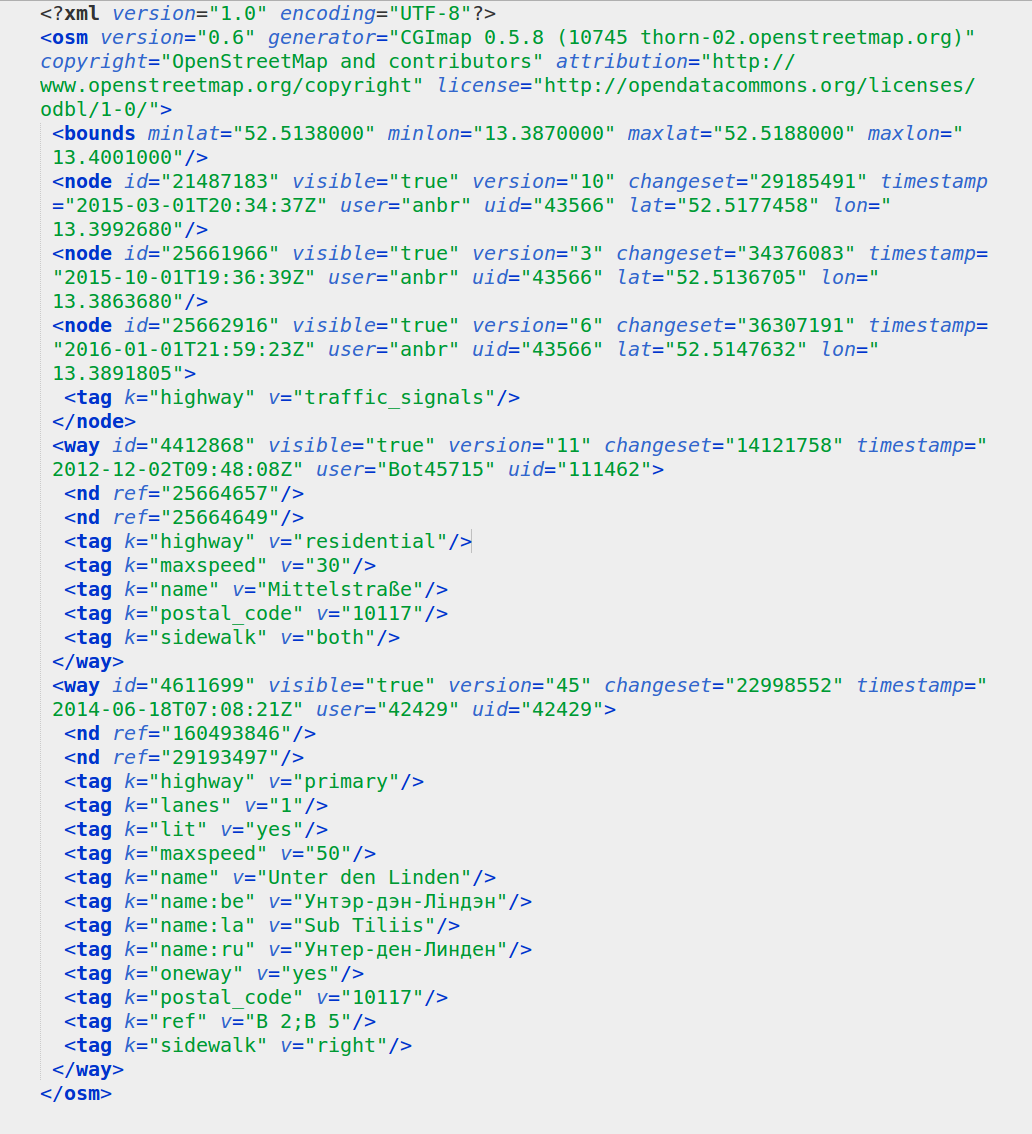
\includegraphics[scale=.478]{osmxml2.png}
\caption{OpenStreetMap XML format example, {\copyright} OpenStreetMap contributors }
\label{fg:osmxml}
\end{figure}

\subsection{OSM: Nodes}
A node is one of the core elements of the OSM data model. It defines a single point on the Earth's surface defined by its latitude and longitude. To allow distinction, a node is always identified by its unique id. Between different versions of a map, a node could be identified by using this id. Additionally, there are other attributes which define other properties of a node. In our example in Figure \ref{fg:osmxml}, these could be seen. Nodes are often used to define the path of the way by referencing them in an order. However, nodes could also be used in OSM, to define location of other objects such as a coffee shop, museum etc. In such cases, an additional set of \textit{tags} are used along with usual node elements. In our example, many attributes could be seen along with the node element. These are described as follows
\begin{enumerate}
\item \textit{id} defines the unique identifier used to identify the node
\item \textit{visible} defines the visibility of the node
\item \textit{version} defines the version of the node in the OSM data-set
\item \textit{changeset} defines the most recent change-set in which this node was added/updated
\item \textit{timestamp} defines the timestamp of change-set in which this node was added/updated
\item \textit{user} refers to the username of the user who added this node
\item \textit{uid} refers to the user's unique id 
\item \textit{lat} refers to the latitude of the location of the node
\item \textit{lon} refers to the longitude of the location of the node
\end{enumerate}
\subsection{OSM: Ways}
A way can be defined as an orderly list of nodes, along with other attributes which define the path's properties. A way can comprise of up to 2000 nodes in sequential order. A closed way, can be defined as the way whose first node is also its last node. Such a closed way could also be used to define a closed area/region. Other ways are referred as open ways which do not have the same first and last nodes. These open ways are used to represent paths, streets, or even highways in a map. Similar to nodes, a way tag in the OSM XML format could have many attributes that define meta information about the way. After meta information, an ordered list of nodes identified by their ids is provided. The correct order of these nodes, define the geometry of the path. Additionally, other information could be appended to a way with the \textit{tag} tags which we describe later. In our example, similar to nodes, a way's attributes can be described as follows
\begin{enumerate}
\item \textit{id} defines the unique identifier used to identify the node
\item \textit{visible} defines the visibility of the node
\item \textit{version} defines the version of the node in the OSM data-set
\item \textit{changeset} defines the most recent change-set in which this node was added/updated
\item \textit{timestamp} defines the timestamp of change-set in which this node was added/updated
\item \textit{user} refers to the username of the user who added this node
\item \textit{uid} refers to the user's unique id 
\end{enumerate}

The \textbf{nd} tags after \textbf{way}, define the order of the nodes. The nodes are referred by their \textit{id}, which are referenced in \textit{ref} attribute of \textbf{nd} tag.
\subsubsection{OSM: Tags} \label{tag}
Followed by the ordered list of nodes to define the geometry of the way, there are multiple entries of \textbf{tag} in our example in Figure \ref{fg:osmxml}. These are used to describe additional features of the way. A way could be associated with multiple such \textbf{tag} entries. Such entry consists of two items, a \textit{key} and a corresponding \textit{value}. The key is referred by attribute \textbf{k} and the value by attribute \textbf{v} in the OSM XML format. The complete list of such tag description could be referenced on OSM's website \cite{tag}. Based on our example, we would explain some of these here.
\begin{enumerate}
\item key '\textit{highway}' describes the category of road defined by the way
\item key '\textit{maxspeed}' describes the maximum legally allowed speed on the way
\item key '\textit{name}' describes the name of the street referenced by the way
\item key '\textit{postal{\_}code}' provides the value of postal code of the region referred by the way
\item key '\textit{lanes}' describes the number of lanes existing on the road
\item key '\textit{name:ISO 639-1 code}' describes the name of the street in corresponding language referenced by the ISO 639-1 code \cite{iso693}, such as 'name:ru' for the name of the street in Russian language
\end{enumerate}

\subsection{Important Attributes}\label{osmattributes}
OpenStreetMap is used in a wide variety of applications. To support all these wide variety of applications, OSM provides a very comprehensive list of features in its format. However, in the scope of this thesis, we have to limit and filter only relevant information for the navigation system. As a result, only selected meta-information about nodes and ways is stored in the database. For example, for \textit{nodes} only id, lat, lon, version and timestamp are selected. Other meta information is discarded. For developing a navigation system based on OSM data, multiple meta-tags related to \textit{ways} are read. However, some such as postal{\_}code, name of the street in another language etc. are discarded. The exact information which is retained in the database after processing can be looked up in Section \ref{dbschema}.
%\section{Source of data}
%\subsection{map daily dumps}
%\subsection{format}

\subsection{Grid Reference} \label{grids}
Similar to a Geographic Coordinate System, grid references can also be used to define locations of points on a map. There are multiple grid systems, with the square grids being the most common one. The axis lines of such grids intersect each other at right angles. Such grids may be arbitrary or can be based on specific distances. For example, two adjacent grids could be 1km apart or 1$^{\circ}$ apart. Depending upon the size of the grid, the grid numbers could be used to identify precisely a point or location on a map. Grid references have found their use in Ordnance survey maps, military maps and various other applications. The smaller the grid-size, the more precisely, it could be used to pinpoint a location / area. Relatively, smaller grid sizes would employ larger numbers for grid references. These references could be universal or region specific based on a fixed reference line. Grid references were very useful in surveying techniques, however with the easy availability of mobile GPS devices, calculating grid references is very easy and accurate. However, it still depends on precision of GPS device.\\



Figure \ref{fg:appgrid} shows an example of such grids. The mobile application \cite{androidapp} is using a grid reference of a rectangle with sides of size 1$^{\circ}$ latitude and 1$^{\circ}$ longitude. For example, the grid marked with 'n52e004' refers to the region between the latitudes +51$^{\circ}$ and +52$^{\circ}$ and the longitudes between +3$^{\circ}$ and +4$^{\circ}$. This grid size is not standard and a smaller grid size could be used by an app. Grid references are used in almost all digital mapping solutions for rendering. However, to optimize the process, such apps use hierarchical grid references with varying size. As one user zooms out, a larger size grid is used to render the map. As you zoom in to the map, multiple smaller sized grid references are used to render high quality details of the map. This technique has been employed since 1980s for digital maps.
\begin{figure}
\centering 
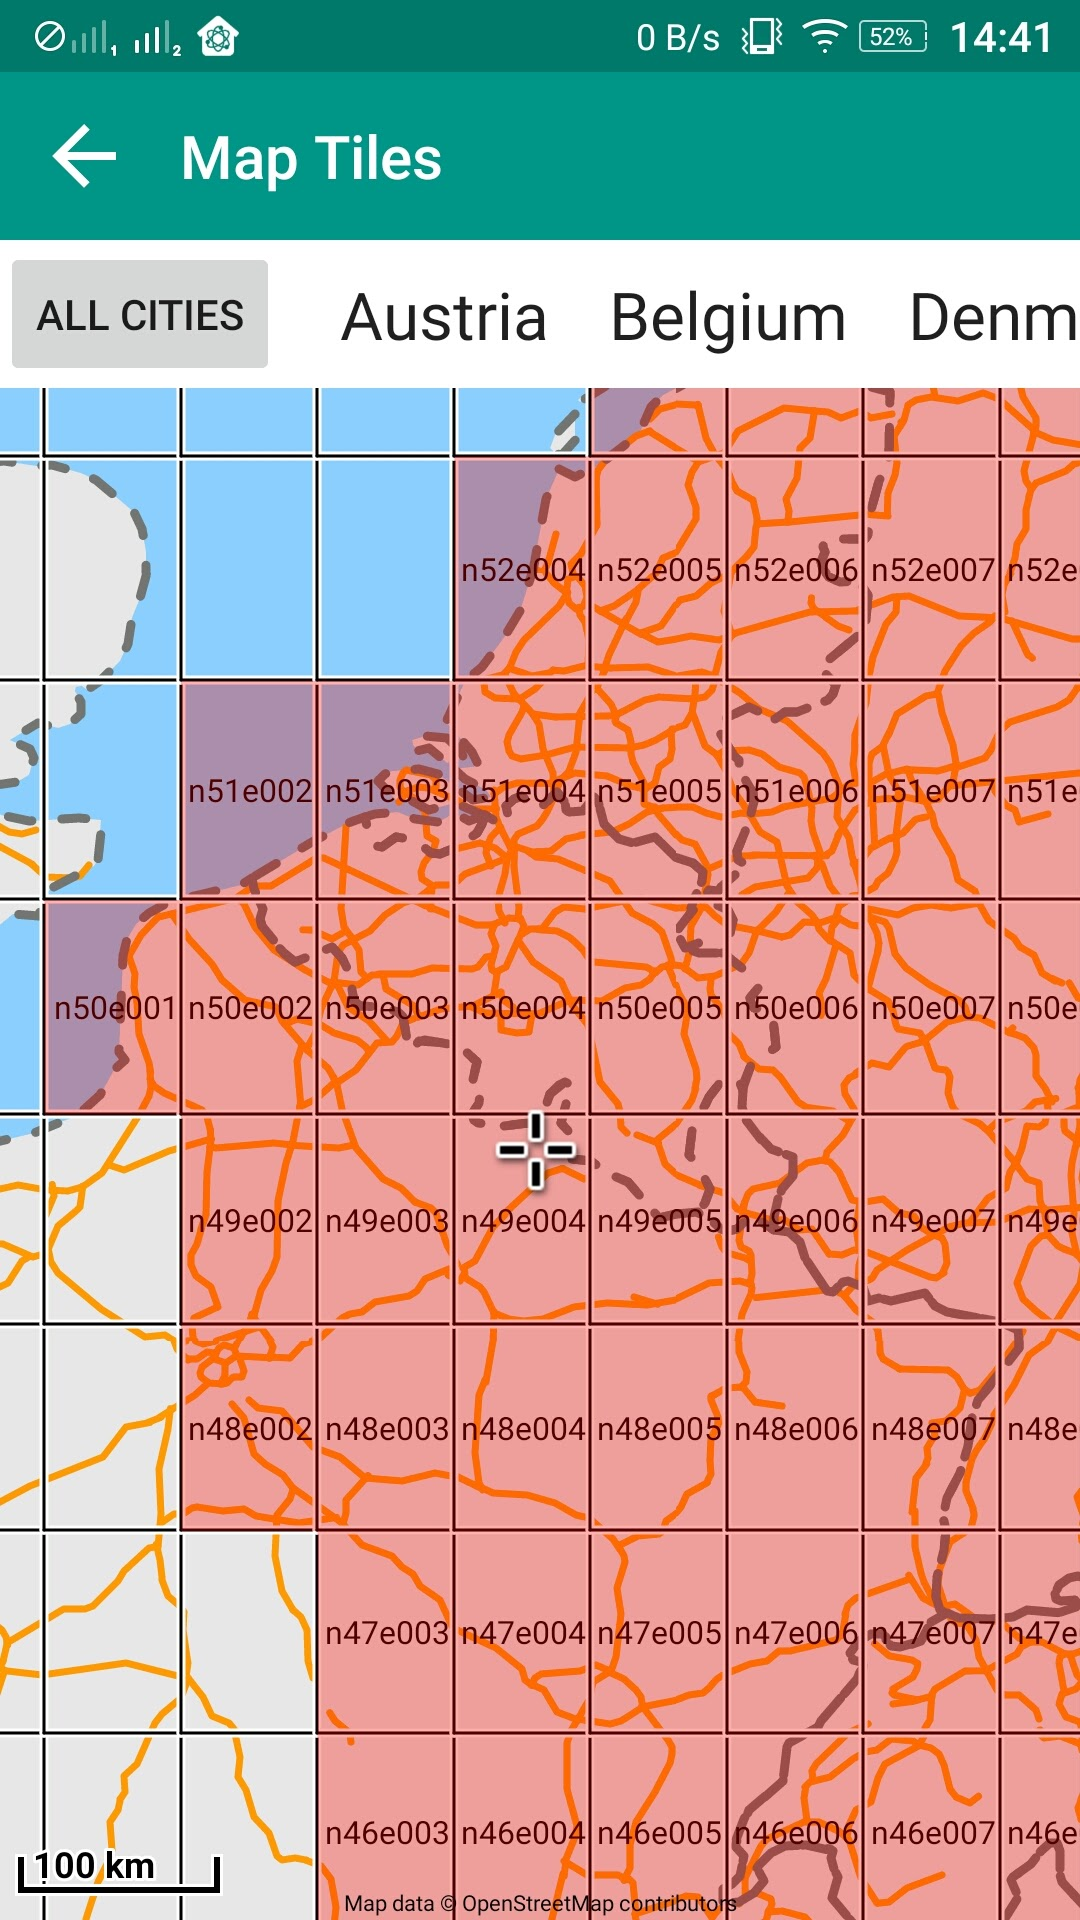
\includegraphics[scale=.15]{appgrids.jpeg}
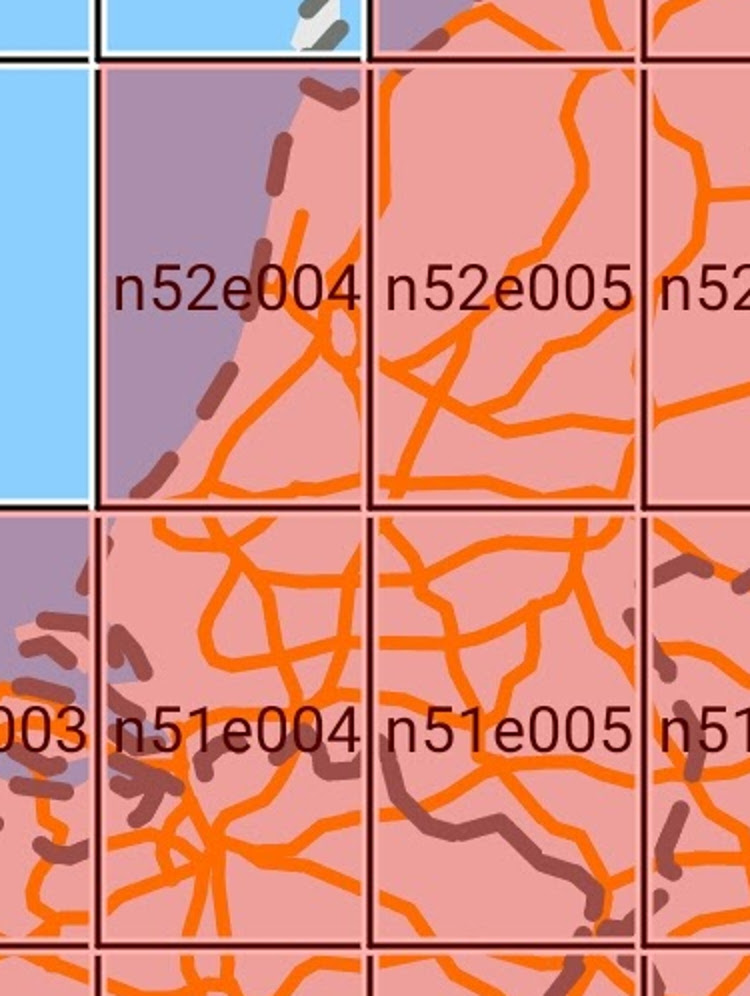
\includegraphics[scale=.25]{appgridsz.jpeg}
\caption{Grid references in mobile app MapFactor GPS Navigation Maps $\cite{androidapp}$}
\label{fg:appgrid}
\end{figure}
\subsection{Geohash} \label{geohash}
Geohash \cite{suwardi2015geohash} is a geocoding system which is a hierarchical spatial data structure. The Geohash encoding scheme sub-divides space into grids of hierarchical buckets. Removal of a character from the end of a geohash results in the loss of precision as it moves to bigger sized grids. Nearby places, could share similar prefixes, not at the edge cases of upper level hierarchies. The latitude and the longitude values of a location are required to get its geohash value. The \textit{precision} factor is a determinant of the length of the geohash. A larger precision value would mean more precise location in terms of the latitude and the longitude. For a low precision value, often values from the latitude and the longitude are truncated. Geohashes have found their use in maps to share unique locations and similarly in databases to represent a specific region i.e. \textit{geotagging}. Geotagging results in faster look-ups for locations as it serves as an index to search queries. Based on the geohash length, the size of the grid it represents could be derived. However, the size of such grids change as the location moves from the equator to the poles. For example, a geohash of size/precision 4, will have a grid of maximum size of 39.1 km by 19.5 km. The size of such grid reduces as you increase a geohash's size/precision. 

\subsection{Spatial Database}
The use of digital maps have led to the development of tools to use them efficiently and easily. There are many applications which use a digital map. To efficiently store and query a digital map, spatial database systems were used. A spatial database \cite{bedard2007multiple} is a database optimized to store and query data representing objects defined in a geometric space. These objects in a geometric space could refer to point, lines and even polygons, however modern spatial databases are designed to even handle complex structures such as 3D objects, linear networks, topological coverages etc.. Spatial databases are similar to typical databases with added functionality to manage and process spatial data types efficiently. Additional features support geometry and other data types in a spatial database. The Open Geospatial Consortium \cite{lupp2008open} released the Simple Features specification \cite{isosfa} to set standards for spatial functionality of such database systems. In addition to typical SQL queries, these spatial operations include \begin{enumerate}
\item Spatial Measurements: Line length, polygon area, distance between geometries etc. calculation
\item Spatial Functions: Existing feature modifications such as bounding boxes, intersecting features etc.
\item Spatial Predicates: Relationship calculations between spatial objects, for examples whether two lines intersect, whether regions overlap etc.
\item Geometry Constructors: New geometric shape creation using vertices
\item Observer Functions: Specific information query method, such as the location of diagonals in a square
\end{enumerate}
To optimize and speed up spatial queries, \textit{Spatial indices} are used by spatial databases. Conventional index types are not designed to handle spatial queries efficiently. %Some of the methods used for spatial index are
%\begin{enumerate}
%\item Grid
%\item Z-order
%\item Quadtree
%\item Octree
%\item UB-tree
%\item R-tree
%\end{enumerate}
Spatial databases are used in wide variety of applications related to Geographic Information Systems (GIS) such as surveying, digital mapping, 3D reconstruction of a surface area. 
\subsection{Shortest Path Algorithms}
One of the common operations with digital maps is finding the shortest route to a destination. In Computer Science, this problem finds its solution in graph theory. In graph theory, the shortest path problem is the problem of finding a path between two nodes (or vertices) in a graph while keeping the sum of weights in the path's edges minimum. The graph considered in the problem can be directed or undirected. \citet{floyd1962algorithm}'s paper presented his algorithm to solve this problem. The problem of finding the shortest path between two points on a map while considering the legal limit for driving on the road presents a special case of the shortest path problem. Multiple scientists have provided a solution to the basic problem of shortest path finding. However, the following are the most important algorithms to solve the shortest path problem
\begin{enumerate}
\item Dijkstra's algorithm
\item A* search algorithm
\item Bellman-Ford algorithm
\end{enumerate}    
Many other important algorithms to solve the shortest path problem and their evaluation can be found in \citet{cherkassky1996shortest}'s paper. In our work, we only used Dijkstra's algorithm which is explained in Section \ref{dijkstra}.
\subsubsection{Dijkstra}\label{dijkstra}
\citet{dijkstra1959note}'s algorithm to find the shortest path between two pairs of nodes in a graph is well known and computes in \textit{O(n$^{2}$)} time. The algorithm is useful in solving many routing related problems in computer science. It has also found many uses outside the field of computer science. In our digital map's context, Dijkstra's algorithm is used to find the shortest path between the source and destination points on a map. The road network from the map data is conceptualized as a graph of nodes and edges. The road connections between two points on a map are referred as an edge between two nodes in a graph. The cost factor of each edge could either be distance between them, or even time taken to cover that distance. The latter could be achieved by knowing the maximum permissible speed for driving on the road connecting the two points in a road network.



%\subsection{A-star}\label{astar}
%Another such algorithm for shortest path problem is A-star or abbreviated as A*. \citet{hart1968formal} formulated this method on top of Dijkstra's previous %work. 


%*****************************************
\chapter{Related work}\label{ch:relatedwork}
%*****************************************

To solve the problems we identified in Chapter \ref{ch:introduction}, many researchers have published their work. The research areas include map representations, change detection and over-the-air map updates. Several different approaches have been suggested by work of \citet{min2008mobile}, \citet{asahara2008locally}, \citet{cooper2001incremental}, Hitachi \cite{hitachi}, \citet{bastiaensen2003actmap}, \citet{sakamoto2000proposal} and the ActMap project \cite{flament2003actmap}. Some of the work in this area also includes work on patents by \citet{kato2002method} and \citet{fischer2012technique} as well. We now present their work and discuss how they solve the problem of differential map updates.



%\nocite{*} % invisibly cite all that is in the bib file! (not a good idea, only for demonstration purposes!)


\section{Navigation Map as a Database} \label{navasdb}
Navigation is one of the most popular mobile services. As discussed in Section \ref{offlinenav}, offline navigation systems use a binary file based format for storing map data. The binary format allows the navigation system to provide speedy route calculations using a relationship based on the file offset values. The binary physical storage format also allows map data to be stored in a very compact format which is one of the requirements for such mobile devices. Existing offline navigation systems (see Section \ref{offlinenav}) use such a proprietary file based format like the KIWI format \cite{kiwiinput}, the GDF format \cite{tc204200214825}, the NAVIKEN format \cite{bullock1994analysis}, etc. for storing navigation data. However, updating such a Physical Storage Format (PSF) is a complex procedure. It requires the whole file to be overwritten to incorporate new changes irrespective of the size of new changes. Another reason for file based navigation data was that the computation power of mobile devices and resources were limited. The recent development in mobile CPUs and lower cost of mobile system on chip designs have changed that. Conventionally, an updated map data or map update is provided every few months by the map provider / device manufacturer to the end user. The complex process of updating such a device has been already explained in Section \ref{existingUpdate}. Typically, the size of changed data is relatively smaller compared to the total map data already stored in the navigation device. Thereby, the process of updating map for smaller changes is inefficient. To overcome this, \citet{min2008mobile} published their concept of navigation data as a mobile spatial database. Their approach allowed partial updating of data to accommodate smaller, however frequent changes in map data in a navigation database. \\

We now discuss \citet{min2008mobile}'s approach to a mobile spatial database for a navigation system. Since, a flash memory is being actively used in mobile devices, they developed a flash memory storage based spatial database management systems (DBMS). They named their software as Flash-aware Ubiquitous Navigation System or FUNs. They categorized data from different use-cases such as routing, rendering and points of interest(POI) into different table-spaces. A table-space corresponds to one file. Using this approach, the routing data could be separated from Point of Interest (POI) data. For example, the location of nearby restaurants is a case of Points of Interest data as only its location is stored. However, to navigate to a nearest restaurant, the location data can be provided as an input for routing function. This approach allows them to partially update POI table structure without affecting routing data in some cases. For example, addition of a new restaurant location in POI data should not affect the navigation on the routes nearby its location. They designed several components of this spatial database system to work independently but in coherence. The system offers SQL-like APIs for various navigation related functions including sound search and k-nearest neighbor search. The system also supports spatial relational operators, such as finding nearest map object to a location as outlined by \citet{lee1998perf}. \\
\begin{figure}
\centering
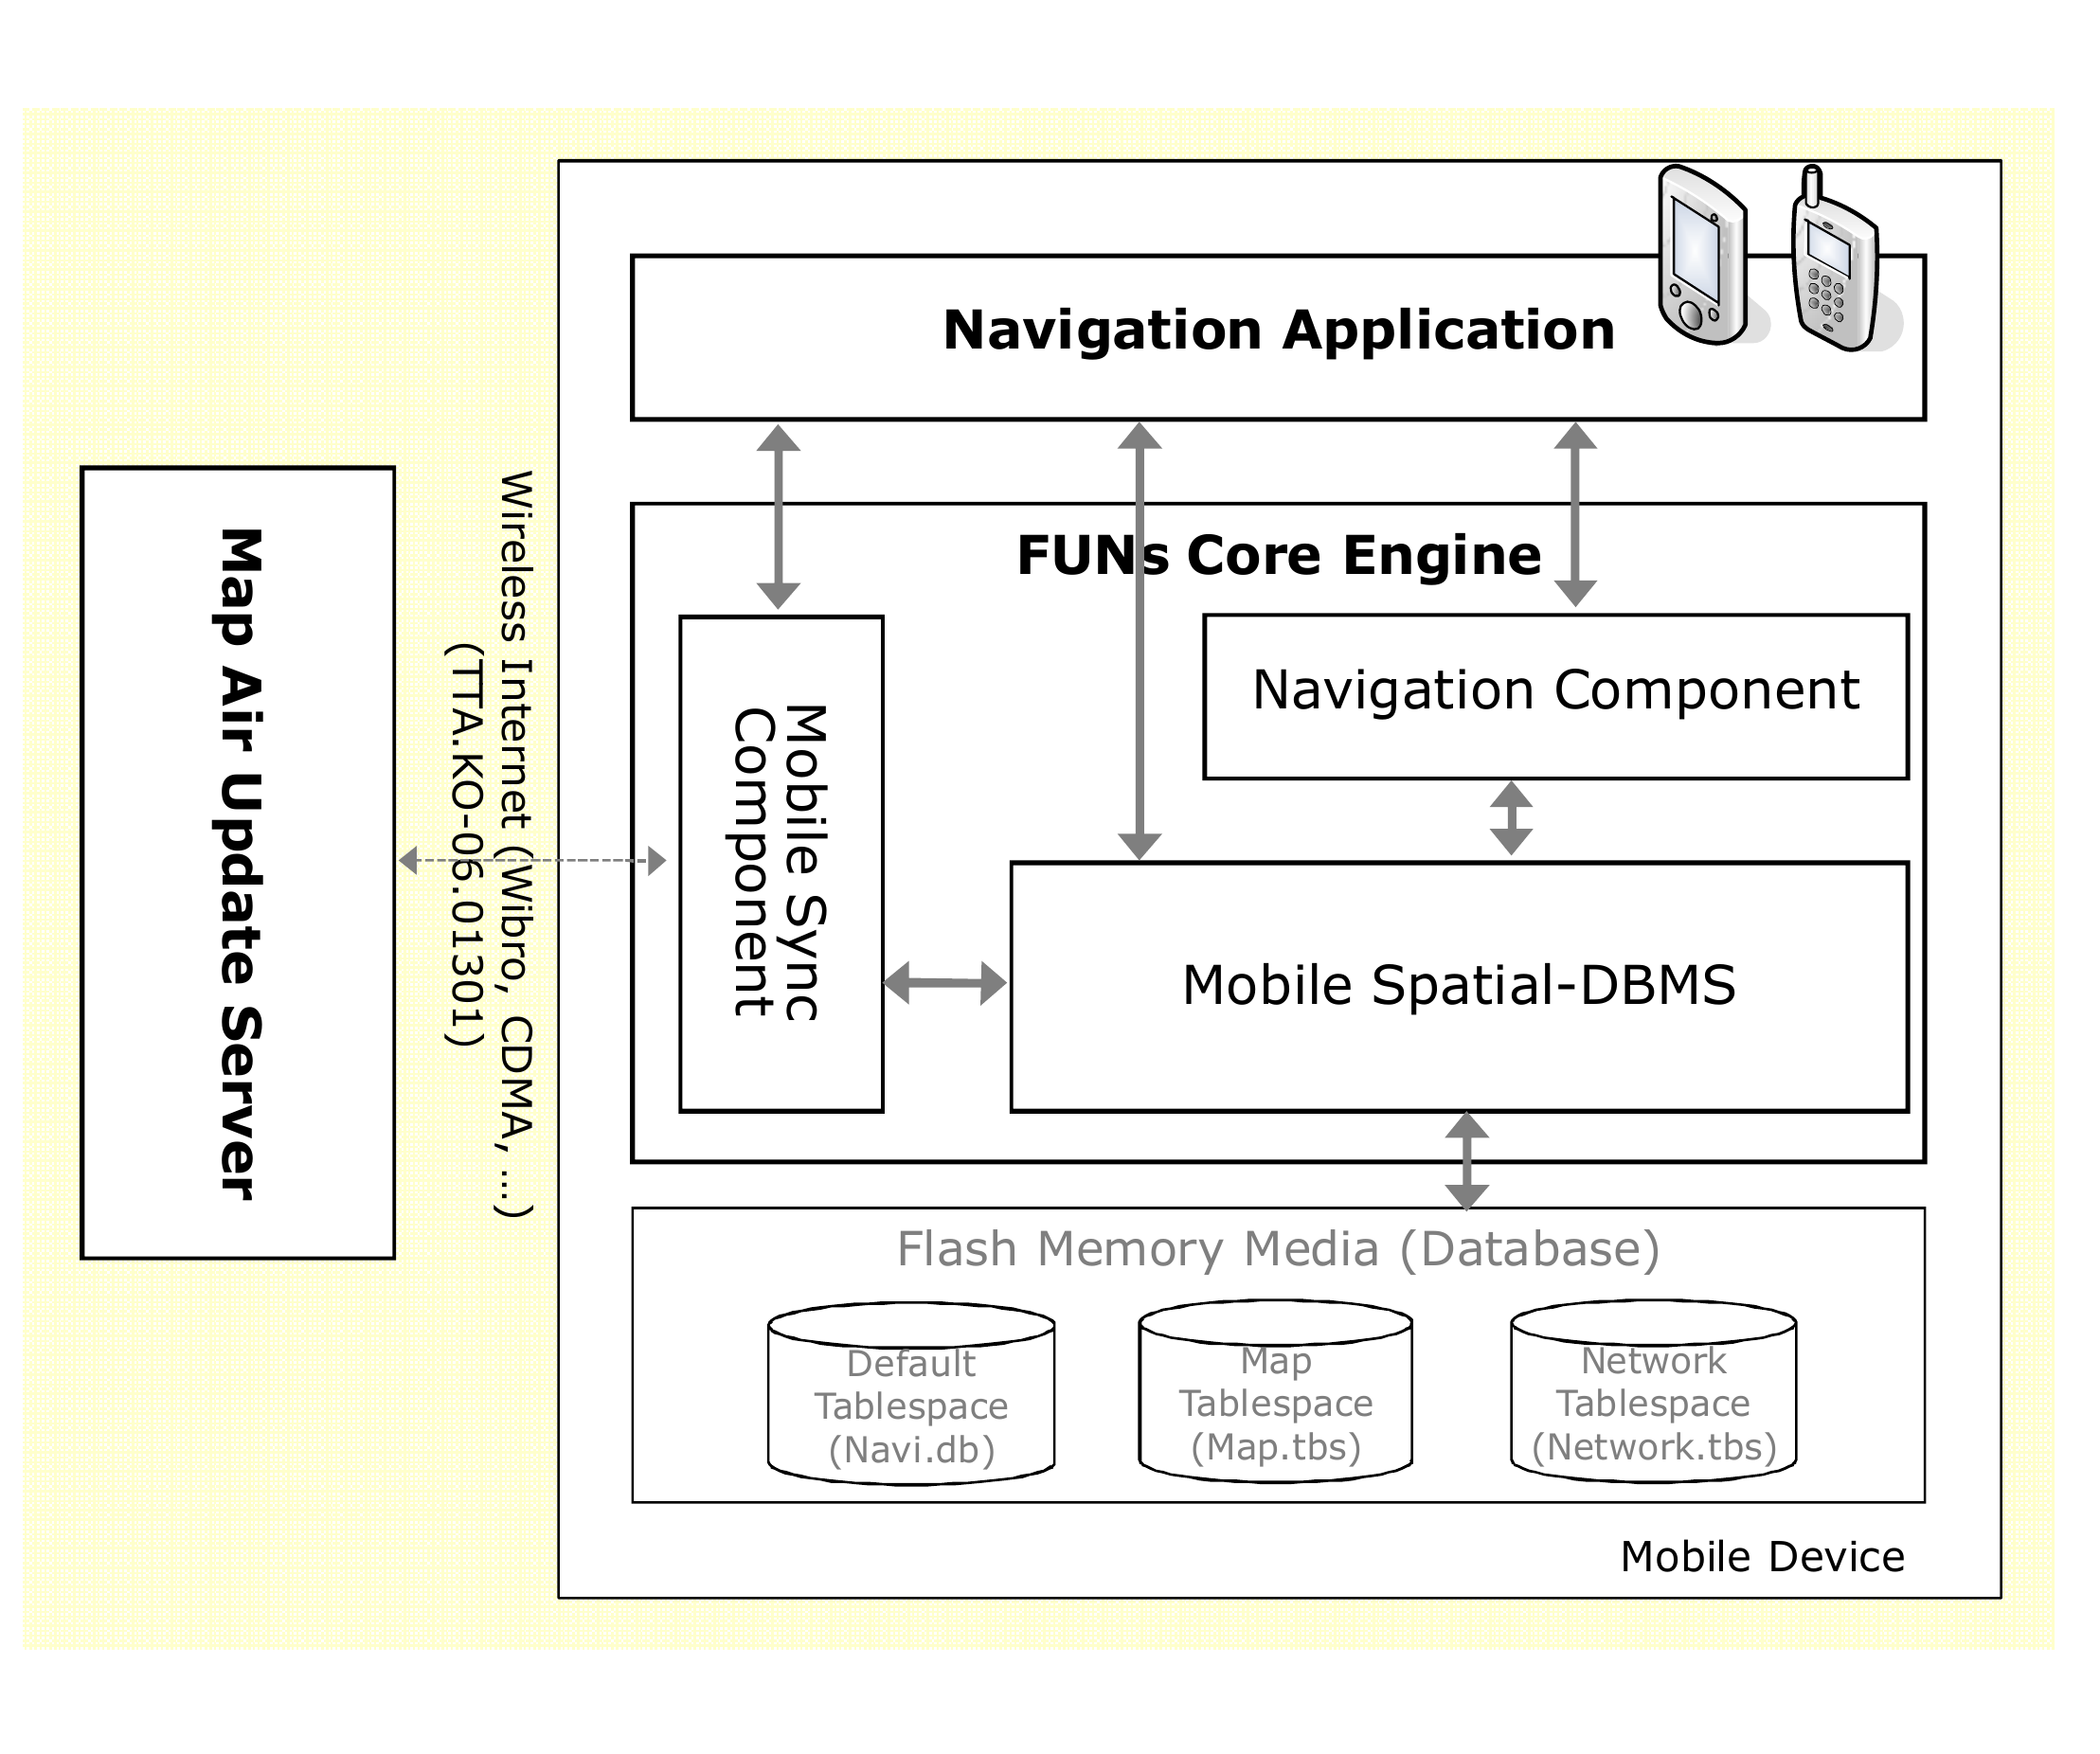
\includegraphics[scale=.23]{FUNsArchitecture.png}
\caption{The System Architecture of FUNs, adopted from Min et al.$\cite{min2008mobile}, \textit{page 3}$.}
\label{fg:sysArchFun}
\end{figure}

Now, we explain how the partial map update is implemented in their design. The system architecture of FUNs is provided in Figure \ref{fg:sysArchFun}. The Mobile Sync component is responsible for updating the navigation database from the partial update provided by a Map Air Update Server (MAUS). The Mobile Sync component allows user to (i) inquire, (ii) subscribe or (iii) unsubscribe from receiving updates for a region of interest. The \textit{inquire} requests allows user to check if there are any updates available for his/her region of interest and if yes, it also returns information about the size of the update and estimated time to download and apply such an update. The \textit{subscription} request allows user to subscribe to map updates for a pre-selected region. Once a subscription request has been made, the navigation devices receives map updates for the selected region as soon as they are available. The \textit{unsubscribe} request allows user to cancel any subscription request he/she may have. They also defined different formats such as BinaryData and ObjectData to deliver these updates. In case of ObjectData, only the components which have to be updated are delivered to the device, thus saving bandwidth costs. Their approach also supports a large update of a completely new region with the use of BinaryData. For example, if traveling to a new country, it would be necessary to download complete map data of new country or at least the major highways and outline using BinaryData. In their experiments, they tested partial map update process as well. The update process was done over cellular network and achieved goals of reducing the update size in kilobytes and it required relatively less time to apply those updates in less 20 seconds \cite{min2008mobile}. We believe that a mobile spatial database which implements partial updates is a good starting point for us towards reaching our goal. However, the existing approach is not sufficient when dealing with high-definition maps. The relatively large amount of map data of a high-definition map requires this approach to be developed further to ensure functionality of a high-definition map over a spatial database. 
%\subsection{Grid based updates}
%<needs input>

\section{The ActMAP Project} \label{actmapprojectsection}
We discussed in our introduction (Chapter \ref{ch:introduction}) that many companies have been specializing in producing navigation systems of a car. We already discussed the benefits of using a Physical Storage Format in earlier section. Additionally, to provide custom key-features and secure navigation devices from tampering, many companies use a proprietary format for storing their navigation data in their devices. This limits the sharing of knowledge about map data and other related information between such map services. Moreover, different data formats are not the only problem, often different devices of the same company had different versions of map data. To provide update to numerous devices, additional overhead is required to process the updated map information into various formats for multiple devices. The Actualize Map or the ActMAP project \cite{flament2003actmap} was a European consortium project aimed at developing standardized mechanisms to update existing navigation databases to enable dynamic content in such navigation systems. The consortium had members like ERTICO, BMW Group, CFR Fiat Research Center, DaimlerChrysler, Navigon, Navteq, Tele atlas, and Siemens VDO Automotive. One of the project's main output was a standard to enable information exchange between multiple proprietary navigation database formats while allowing them to exchange information such as an updated list of Points of Interests (POIs) between them. The project submitted their specification \cite{flament2003actmap} and evaluated with a proof-of-concept design. However, the project failed to commercialize. The ActMAP project's incremental updates design is based on fixed, constant reference IDs. If they change, it can not work properly. However, when a map company generates a newer version of a map, they re-assign all the reference IDs during compilation. This prohibited any ActMAP format to work correct on such a proprietary format for incremental updates. This could be attributed as one of the reasons which led to failure of the ActMAP project.\\

Now, we discuss briefly the design and contributions of the ActMAP project, however we would largely focus on their incremental update approaches. One of the important part of ActMAP specification is the ActMAP update exchange format. It is an XML-based format to exchange map updates between various proprietary formats. The specification was designed to support all of the proprietary map database formats supplied by consortium members. The map data is split into multiple layers based upon their different applications. By separating the map data into multiple layers, a partial data update was possible. Multiple different approaches to minimize the update data size were considered. One of them is updating only a specific monitored geographical region such as a state or a small country. By having a relatively smaller geographical region, the map data could be updated over a cellular connection. However, the version information of every map object inside a map database is required to be known. A version control is necessary to make sure that partial updates can be applied in a correct order to work properly. \\

\begin{figure}
\centering
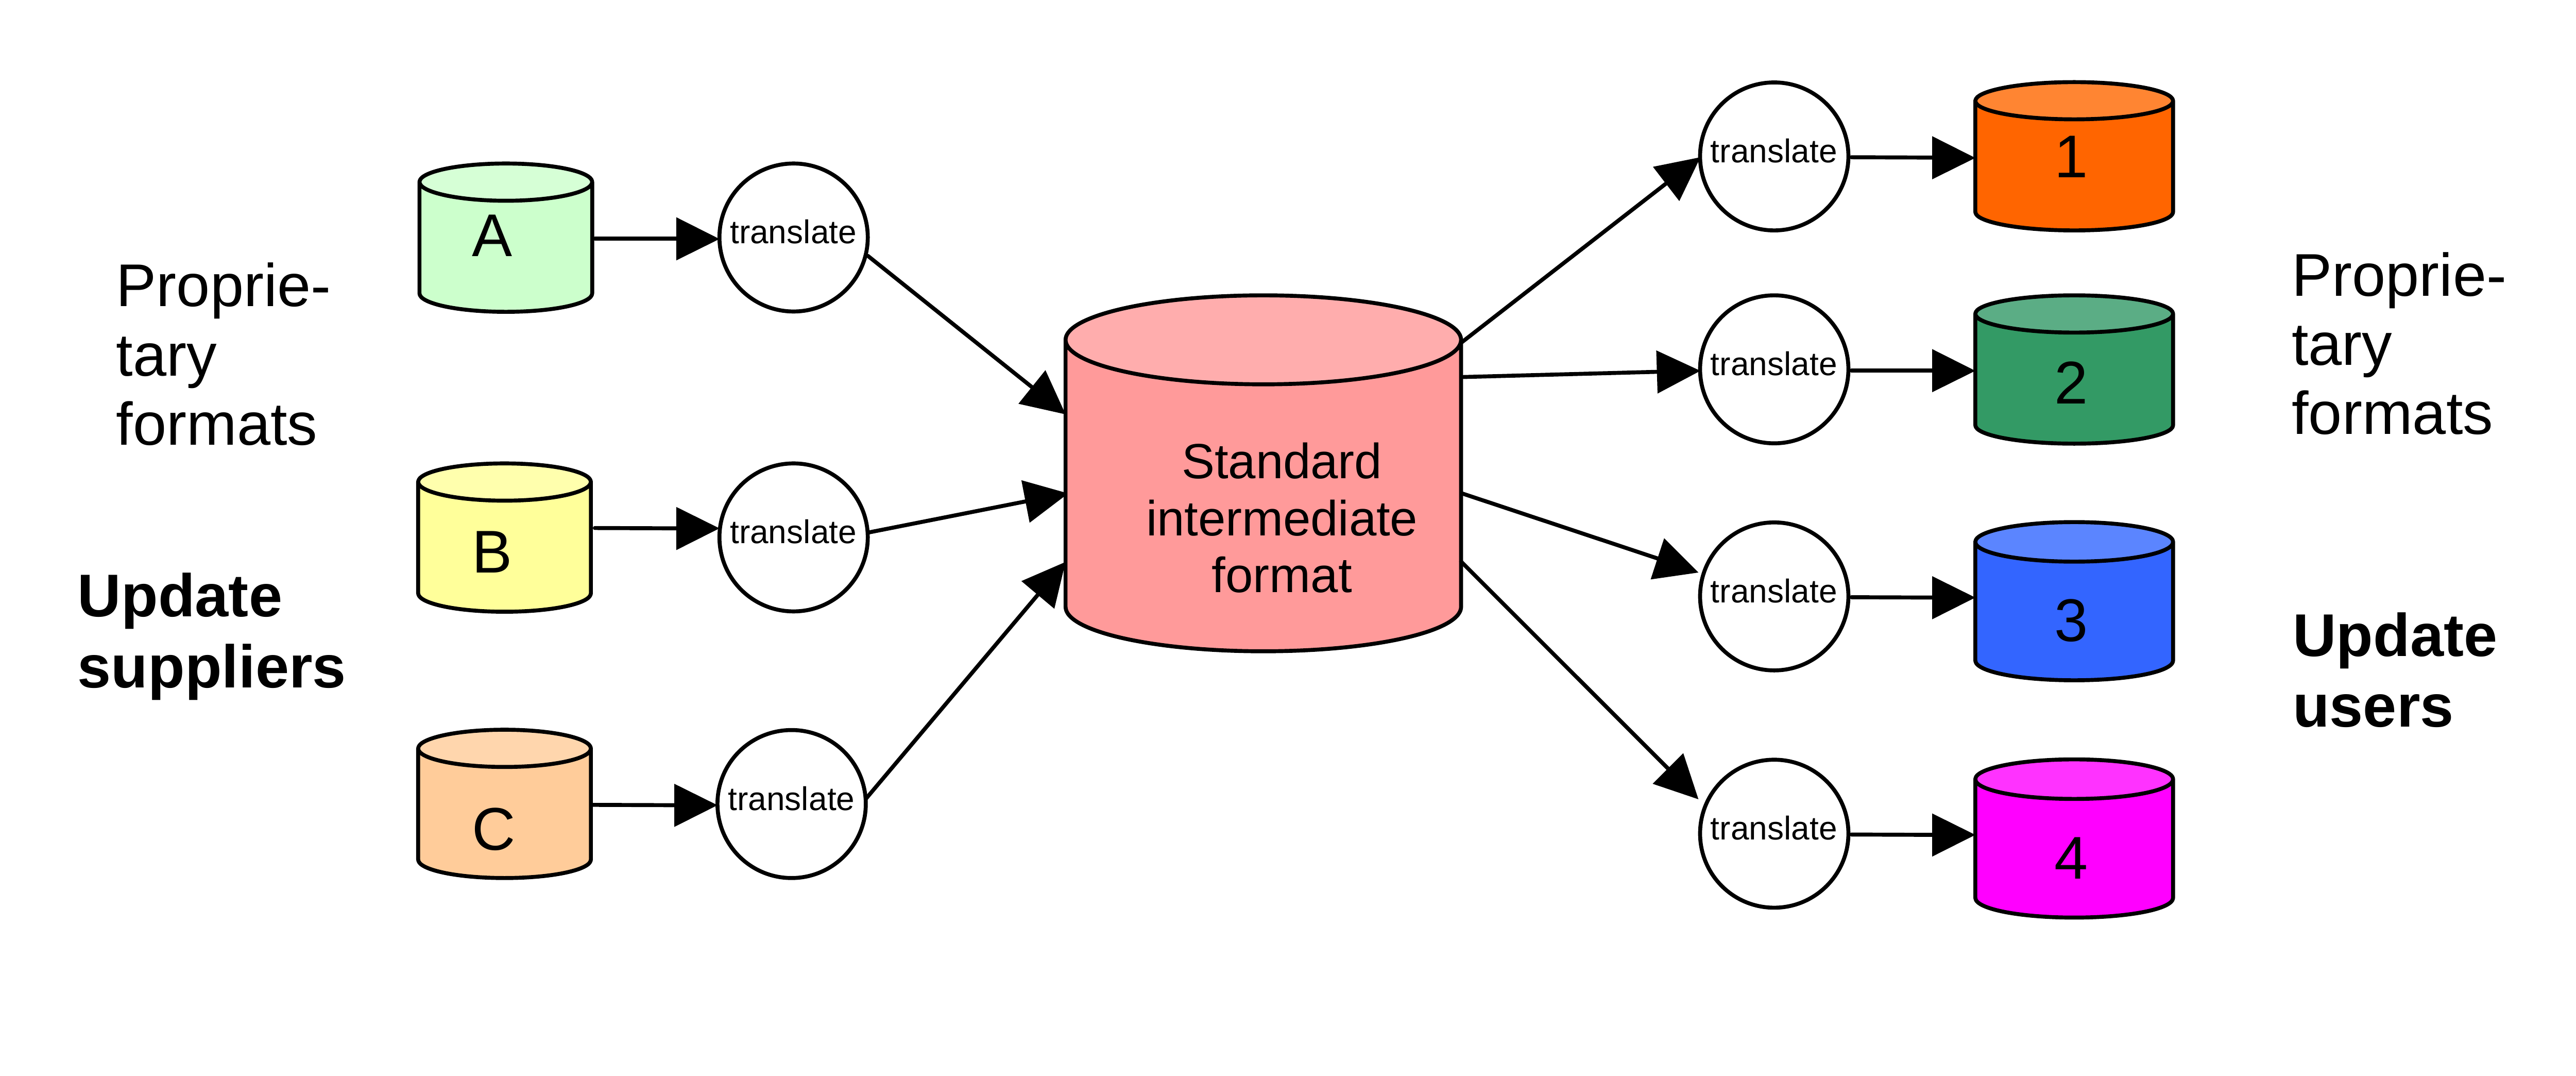
\includegraphics[scale=.13]{ActMapExchange.png}
\caption{ActMAP Standard Intermediate Format, adopted from $\cite{flament2003actmap}, \textit{page 25}$}
\label{fg:actmap}
\end{figure}

As depicted in Figure \ref{fg:actmap}, the ActMAP project produced a standard intermediate format for exchanging update information. The main motive behind such a format was to allow the exchange of information between different mapping companies and their different formats while maintainig them in their internal storage map database formats. The ActMap project's intermediate format reduced the number of conversion engines between various formats of the map data. For example, for 'n' update suppliers to provide update for 'm' different devices, each with their own proprietary format, normally the number of required conversions is 'n $\times$ m'. However, with the use of an intermediate standard format, the number is limited to only 'n + m' conversion engines. This is one of the key achievements of the ActMAP's specification. It allows all participatory map makers to provide a common format in intermediate specification, which could be shared between a map server and a car or even a car to another car to allow map updates. The standard intermediate format was designed to enable the exchange of map descriptions unambiguously. The translation of such a standard format into proprietary database would not require much changes as the difference is not too large \cite{flament2003actmap}. For offline update of map database of an offline navigation systems, the ActMAP project described their novel method which was later referred in works of \citet{sakamoto2000proposal} and \citet{asahara2008locally}. They used unique identifiers of map objects and associated attributes to them. These map objects could be added, deleted or updated in the next update cycle. This resulted in tremendous reduction in size of update for such an offline system, as only the changes were required to be configured in the update. If only one attribute of a map object has changed, this would result in adding just map object's unique ID and associated attribute changes to the update file. If referencing map objects was not possible due to change of unique IDs in newer version of the map, the specification allows use of generic referencing methods such as AGORA \cite{hummelsheimlocation} or ROSA \cite{demir2002new}.

%\section{Existing update approaches}
%In this Section, we would discuss some of the novel approaches to detect and deliver map updates for a navigation system. We would also discuss their design principles upto some extent.
\section{Incremental Updates and Version}\label{incrementalupdates}
In previous section, we discussed the ActMap project (Section \ref{actmapprojectsection}) and how it uses version information to minimize the update required instead of overwriting as in the case of the Physical Storage Format (PSF). We now look at another approach to handle changes between different versions of a map data. The data in a geographical information system such as a navigation device has many different purposes. We would see later in Section \ref{nds}, how different information displayed on a navigation device are stored. We understand from previous discussions (Section \ref{navasdb}) about how navigation data could be stored in a mobile database and partially updated. We also understand that map data providers periodically provide update for map systems. Typically, it was designed to completely overwrite the map data files. With overwriting, no versioning system was required. Such overwriting allowed a device to be easily overwritten even to an older map data. Even though the map provider was providing updates, it was the user's responsibility to understand and maintain different versions of map data. The user would have to understand and apply updates in correct order. In some cases, ignoring an update is also possible by user. Selective updates were also allowed. However, to build a system to support an autonomous car's high-definition maps and their constant updates, it requires some versioning system to identify the locally stored map data and to allow processing to generate a partial or complete update. \citet{cooper2001incremental}'s work provides an insight on what are the requirements of such a versioning system. Their work inspires us to have a proper versioning system in our approach as discussed in Chapter \ref{ch:approach}. \\

\citet{cooper2001incremental} outline the problem of incremental map updates and versioning. They argue that a framework for such versioning should be able to fulfill requirements for different professional associated with the generation of map data. The framework should be able to resolve any disputes arising from partial updates and local data. They argue that since data in a spatial database is divided into different sets providing different services, there should be a different versioning for the core data. In addition to that, partial updates could have different versioning on top of the core data sets which is regularly maintained. They present their approach of comparing two different versions which differ in time as "vertical". Additionally, different data extracted from same base data was referred as "lateral". Cadastral data vs transport networks extracted from same base data set would be an example. They also discuss dividing data into two main aspects for versioning. They argue that some of the data lies in temporal domain, the data set which might be valid for only a small time. A temporary diversion of a route due to an accident, a traffic jam at certain junction etc. could be classified into temporal domain as it is valid only for a period of time. Variation in such a temporal data is inversely proportional to its size. A traffic jam situation on a small junction is likely to change more often than a nation's border. They call it the data set's temporal domain or DSTD. They also present a second temporal domain for datasets which they refer to as the cartographer's temporal domain or CTD. CTD represents the period during which the data is recorded by the cartographer. A recently added highway or bridge or a road which was recently extended would lie in CTD. The CTD implies that the cartographer had previous knowledge about the map data and the changes are corrections or additions to that. Please note that a cartographer in such a case could be a group of different professionals or even an automated system used to generate newer map data. \cite{cooper2001incremental}'s approach of classification of map data set in order to properly version them is an important requirement for delivering partial updates for high-definition maps. 

\section{Connection Maintained - Locally Differential Map Update} \label{cmldmu}
Earlier in Section \ref{actmapprojectsection}, we discussed Differential Map Updates concept in relation with the ActMap project. The differential map update method results in savings as only the changed information is required to be transmitted. Building upon that, we discussed versioning approaches in Section \ref{incrementalupdates}. However, Differential Map Updates approach can result in some consistency issues. We will now present one of the issues related to Differential Map Updates regarding the consistency of the map data. We would also present \citet{asahara2008locally}'s work which deals with the problem. \citet{sakamoto2000proposal}'s work about Differential Map Update (DMU) methods provides an initial overview of how differential map updates could be used to save bandwidth while updating a particular region of the map. However, the DMU methods fail to provide a perfect solution for rapidly changing map data. They used complex indexes and many variations of index keys which complicated the whole process of updating. Because of the complex update process, it took longer than expected to update and the application was unavailable while the update process was executing. \citet{asahara2008locally} investigated \citet{sakamoto2000proposal}'s work further in their paper. \citet{asahara2008locally}'s work builds upon DMU and suggests to develop a better Locally Differential Map Update (LDMU) methods based on findings by \citet{flament2005results} on the ActMap project\cite{flament2003actmap}. The suggested work provides a faster update process by avoiding cascading updates while still keeping the map data consistent. Such a LDMU method required navigation system to use a database for its data similar to the one described earlier in Section \ref{navasdb}. \\

We now discuss \citet{asahara2008locally}'s work on Connection Maintained - Locally Differential Map Update (CM-LDMU). Their work imagines every map object to have a unique ID which could be referred by ID(\textit{m}). This ID could be used to retrieve other attributes of a particular map object. All the other map objects linked to a map object can be queried by using ref(\textit{m}) where \textit{m} is the map object. A map consists of a set of such map objects. For versioning, the first version of a map is referred by M$_{1}$. Map versions increase over time with an increment of 1 whenever the map object changes. If a map object \textit{m} has not changed, between two different versions of a map, \textit{m}$_{i}$ = \textit{m}$_{j}$. Using Differential Map-Update (DMU) method, the differences between two map versions was classified into three types: 
\begin{enumerate}
\item new map objects which are to be added in the newer version of the map,
\item old map objects which are to be deleted in newer version of the map, and 
\item update map objects which already exist in both the old and new map.
\end{enumerate}
Applying this approach to a confined region pre-selected by navigation system or the user, greatly reduced the amount of update required by a navigation device. Table \ref{reduction} provides an insight into the amount of savings that can be achieved by employing Differential Map-Update method over two regions, Spain and Luxembourg. Conveniently, a map could be divided squarely into areas known as parcels. Parcels are synonymous to the grids described earlier in Section \ref{grids}. The differences as described earlier, between two map versions could be calculated for a local region and downloaded over a cellular network and applied to the navigation system. However, such a Locally Differential Map Update method had one quirky issue. In cases where a road link was crossing into boundaries of two parcels, the road link was divided and two new points for both parcels were generated and stored. This resulted in broken updates. In cases, where an old road link had to be deleted, it would be deleted in one parcel, leaving the second connected parcel unchanged. This would result in inconsistent map state. \citet{asahara2008locally} proposed a solution to this problem. They proposed that the road-links which are related to each other should be all updated at the same time. This could lead an update of one parcel, resulting into an update chain of many parcels if they have connected road-links spanning between two neighboring parcels. So, in order to update a parcel, navigation system would have to check all the map objects which have changed. After checking that, it has to check for related map objects which might exists in other parcels. This could be achieved by using attribute ref(\textit{m}). Such a system which created dependency check before actually applying updates, fixed the consistency issue arising from LDMU methods. Asahara et al.'s CM-LDMU method is a novel idea on maintaining consistency while applying differential map update. It might lead to some extra bandwidth usage than LDMU methods, however the consistency of a map would be retained even after a map update, which is important while designing an update process.

\begin{table}[]
\centering
\begin{tabular}{|l|c|c|c|c|}
\hline
\textbf{Region}              & \multicolumn{1}{l|}{\textbf{Inserts}} & \multicolumn{1}{l|}{\textbf{Delete}} & \multicolumn{1}{l|}{\textbf{Updated}} & \multicolumn{1}{l|}{\textbf{Total}} \\ \hline
\textit{\textbf{Spain}}      & 14\%                                  & 6\%                                  & 10\%                                  & 30\%                                \\ \hline
\textit{\textbf{Luxembourg}} & 5\%                                   & 4\%                                  & 6\%                                   & 15\%                                \\ \hline
\end{tabular}
\caption{Change rates of two different regions, adopted from the ActMAP Project $\cite{flament2003actmap}, \textit{page 40}$}
\label{reduction}
\end{table}

\section{Map Air Update Service}\label{maus}
In Section \ref{navasdb}, we discussed how a mobile spatial database could provide a better alternative to store navigation data than a physical file format. Although many navigation systems started using a mobile spatial database to store map data, it was not completely optimized for delivering the same level of performance after many updates. Also, a navigation request performance was not up to the mark as it would turn into repetitive query-by-query searches of nodes and links on the computing route in DBMS. To overcome such issues, \citet{min2011system} presented their approach towards as framework design in which they optimized not only their mobile spatial DBMS but also provided a method to update map data from a server. Their work specifically focuses on partial map updates and performance improvement in mobile spatial DBMS. Their work utilizes their earlier design of mobile spatial database \cite{min2008mobile}. They have proposed a DBMS design similar to spatial main-memory DBMS (MMDBMS) design by \citet{yun2005development} which utilizes the main memory of a mobile device as a storage media. However, in their case it uses flash-storage to provide spatial-data type using the extension of legacy relational DBMS. \\

\begin{figure}
\centering
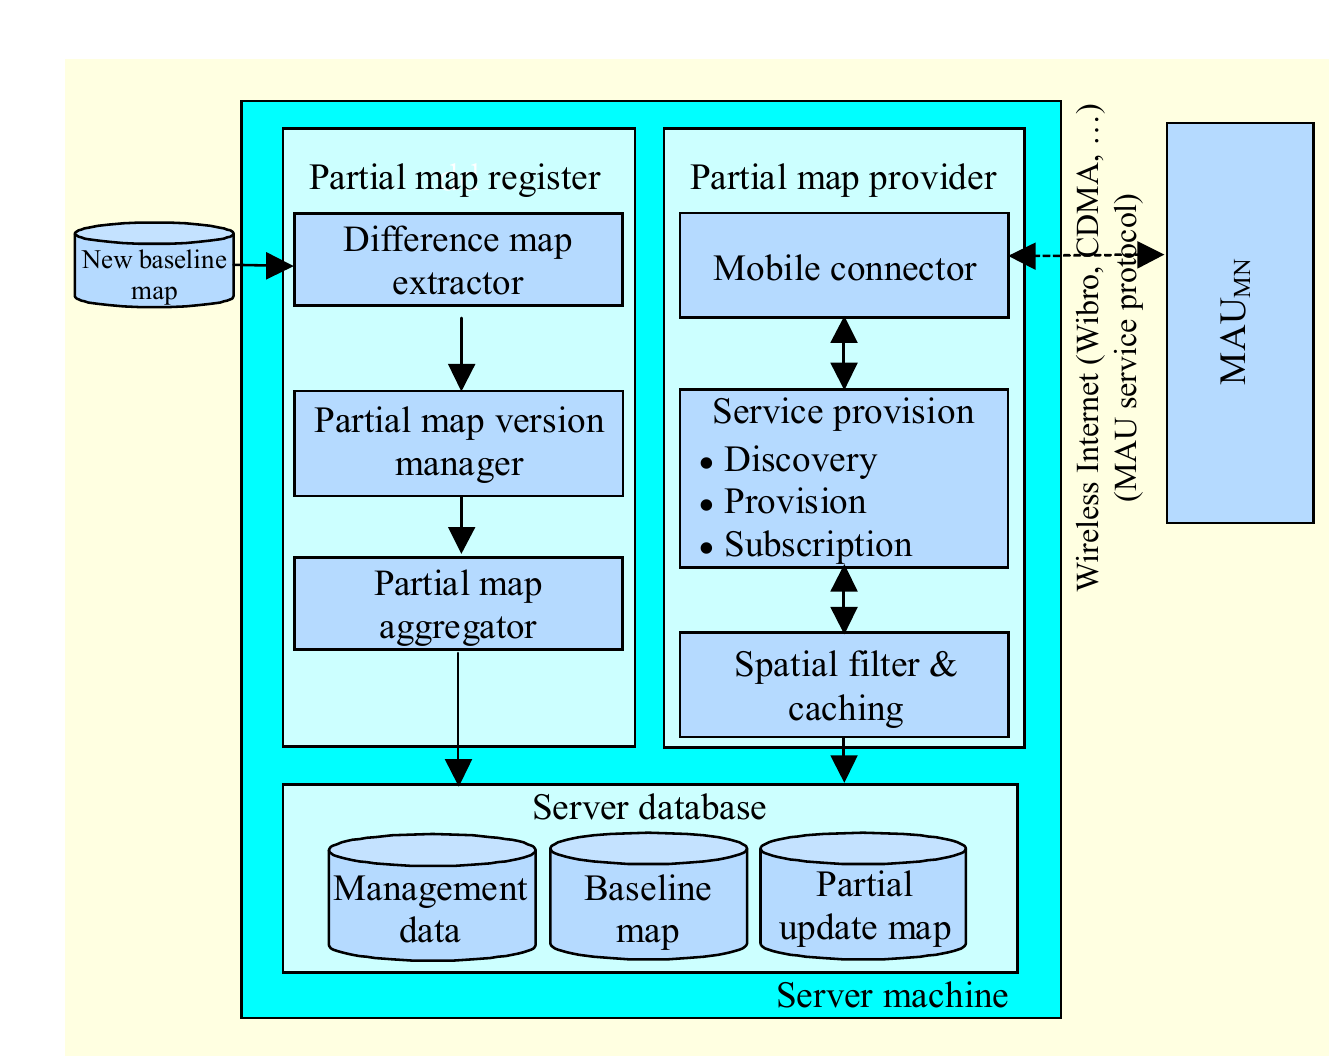
\includegraphics[scale=.4]{MAU_Architecture.png}
\caption{Map Air Update System Architecture, adopted from Min et al.$\cite{min2011system}, \textit{page 4}$}
\label{fg:maus}
\end{figure}
For partially updating a mobile database, \citet{min2011system} have designed a Map Air Update Service and defined an XML-based protocol for request and response while communicating with a update server. A so called \textit{Discovery service} supported by the protocol allows a mobile navigation system to check for updates, get a summary about the available updates. A second service, the \textit{Provision service} allows user to request update of any defined region by the user. A third service, the \textit{Subscription service} provides an option to directly receive push notifications if an update is available, rather than a push service. According to the protocol, if a mobile navigation system requests for update for a specific region, it provides the version of the area it has available locally. Upon receiving such request and depending upon the type of service request, the Map Air Update (MAU) Server calculates partial updates for the requested region from the version supplied in the request to the most recent version available at the server. The difference between the version of map data available at navigation device and the latest version at the server side is extracted by \textit{Difference map extractor} running at MAU server, see Figure \ref{fg:maus}. The update only includes the information about the map objects existing in the requested area which have been either modified, deleted or newly added in that area. The aggregated update includes only the difference between the old version at navigation system and the current version skipping all the intermediate versions of map data. Such an update by the MAU server eliminates the necessity of applying updates in a sequential order. This is useful in cases where the user has not updated the map data for several days and there are multiple versions between the version available at navigation system and the version available at MAU server. The intermediate versions of the map objects can be neglected and saves the bandwidth as those changes are not transmitted in the aggregated map updates. The modified mobile database system provided by \citet{min2011system} improves route searching algorithm as well. The most popular route searching algorithms such as Dijkstra (Section \ref{dijkstra}) and A* have been implemented in their mobile spatial DBMS design. They take advantage of multilevel network data table design of spatial DBMS. The road network is divided into multiple layers from level 1..n, level 1 being most important roads down to level n for residential streets. For finding a route between points A and B, if A \& B both lie at level 1 in the road network, the DBMS would use level 1 routing to find path between A \& B. If the source and the destination points lie in different layers, the algorithm uses information of routing at different levels and to boundary nodes between those layers to generate a preferred route between the source and the destination.



\section{Hitachi Automotive Systems}
As discussed in Section \ref{cmldmu}, maintaining a map's consistency while partially updating it can lead to overhead. The general approach of updating map tile by tile is not very efficient. Members of Hitachi Automotive Systems, Ltd. \cite{hitachi} claim that the general approach of updating individual map tiles as proposed by Asahara et al. leads to unwanted "updating cascades". This means, if one map tile gets updated the neighboring map tiles also have to be updated to ensure the routing capability of the map. The cascades then lead to unnecessary control data traffic over the network for the exchange of further map updates. To solve this problem they propose a different map update approach. Instead of updating specific map tiles, the updates are provided through individual map update objects. They consist of all the changes that have to be applied to a certain, connected area of the map. Thus no individual updates of all the affected map tiles are necessary. The amount of data needed to store the update information is also reduced. \\

Additionally, \citet{min2011system}'s work provides an insight into updating service which provides updates via three different services. Their work does not discuss consistency in general, however the \textit{Discovery Service} can be seen as a way to avoid consistency issues by checking the map updates available for a particular region. We have covered this in Section \ref{maus}. In the next section, we now discuss Navigation Data Standard (NDS) which has been designed from the ground up to allow map updates. We will also discuss the map update process for NDS.



\section{Navigation Data Standard} \label{nds}
We discussed in Section \ref{navasdb} how and why navigation systems providers choose proprietary binary formats for storing map and navigation data in their devices. 
We also discussed how complex and lengthy updating a map data could be if it uses proprietary binary formats. 
Sometimes it could even take upto 2 hours to update the map data on a navigation system. 
To overcome such a situation, \citet{min2008mobile} proposed a mobile spatial database which we explained in Section \ref{navasdb}. 
We already discussed how beneficial such a move from proprietary binary format to a mobile spatial database can improve the update process while maintaining performance similar to a binary format of navigation data. 
However, the lack of a common format for such mobile spatial database restricted the update process to be controlled by the device manufacturers. 
The Navigation Data Standard (NDS) by \citet{muller2010navigation} is an approach to overcome different formats used by different map providers, be it a map maker or a navigation systems supplier or even a car manufacturer. 
Navigation Data Standard (NDS) e.V. is a registered German society of car manufacturers, map developers and navigation systems suppliers. 
The NDS aims to reduce the cost of maintaining proprietary storage formats by standardizing a map format. 
By standardizing the map format, it allows different manufacturers or map makers to provide seamless update and share knowledge within the association while reducing costs. 
The NDS has been gaining popularity worldwide as the members includes large car manufacturers such as the BMW Group, Daimler, Hyundai, Volvo, Volkswagen and map makers such as TomTom, AutoNavi, NavInfo, HERE and even navigation systems suppliers such as Panasonic, Alpine, Garmin, Harman, Denso etc. 
The list of members of the NDS Association is not just limited to these three types of companies. 
The list also includes developers and potential service providers such as Baidu Inc. The services provided by such companies include safety services, vehicle tracking in case of theft etc.   
The NDS Association is focused to innovate for the future for accepting challenges of autonomous driving while increasing adoption worldwide.\\

The standard allows the easy exchange of map data information between different systems conforming to NDS. The map and navigation data is separated from the application software in NDS. Thereby, serving a common platform of developers or service providers to build compatible applications for everyone. The ever increasing adoption of NDS worldwide provides many benefits such as faster map updates, sharing of incident reports, reduced costs to the services providers as well as the consumers. However, in our problem context, NDS supplies a harmonized format for different navigation systems which is designed to support frequent map updates. To make it future-proof, the NDS has been modified to support high-definition maps required for the autonomous cars as well. We now discuss how NDS would benefit in terms of the map update process, comparing it to earlier methods as described in Section \ref{existingUpdate}. 

\subsection{How NDS Allows Updates}
We discussed how NDS delivers a new common standard for navigation data and software. We now explain some of the general working principle of NDS in detail. To allow easy updates of a map database while maintaining fast file based access, NDS uses SQLite database file format. An NDS database would internally have many databases inside it. The federation allows NDS databases to support specialized features from different companies. It also supports flexible and consistent versioning concept. Thus NDS also supports incremental map updates. The inner structure of the smaller databases are always NDS compliant. The smaller databases could be further specified by their levels and so called building blocks. The building blocks in NDS refer to different functionalities supported by NDS \cite{ndsblocks}. For example, points of interest, routing information and traffic information. Figure 3.4 shows an overview of how such blocks come into play in a navigation system. Such a system, helps further partial updating of components inside a navigation system via over-the-air updates.  \\
\begin{figure}
\centering
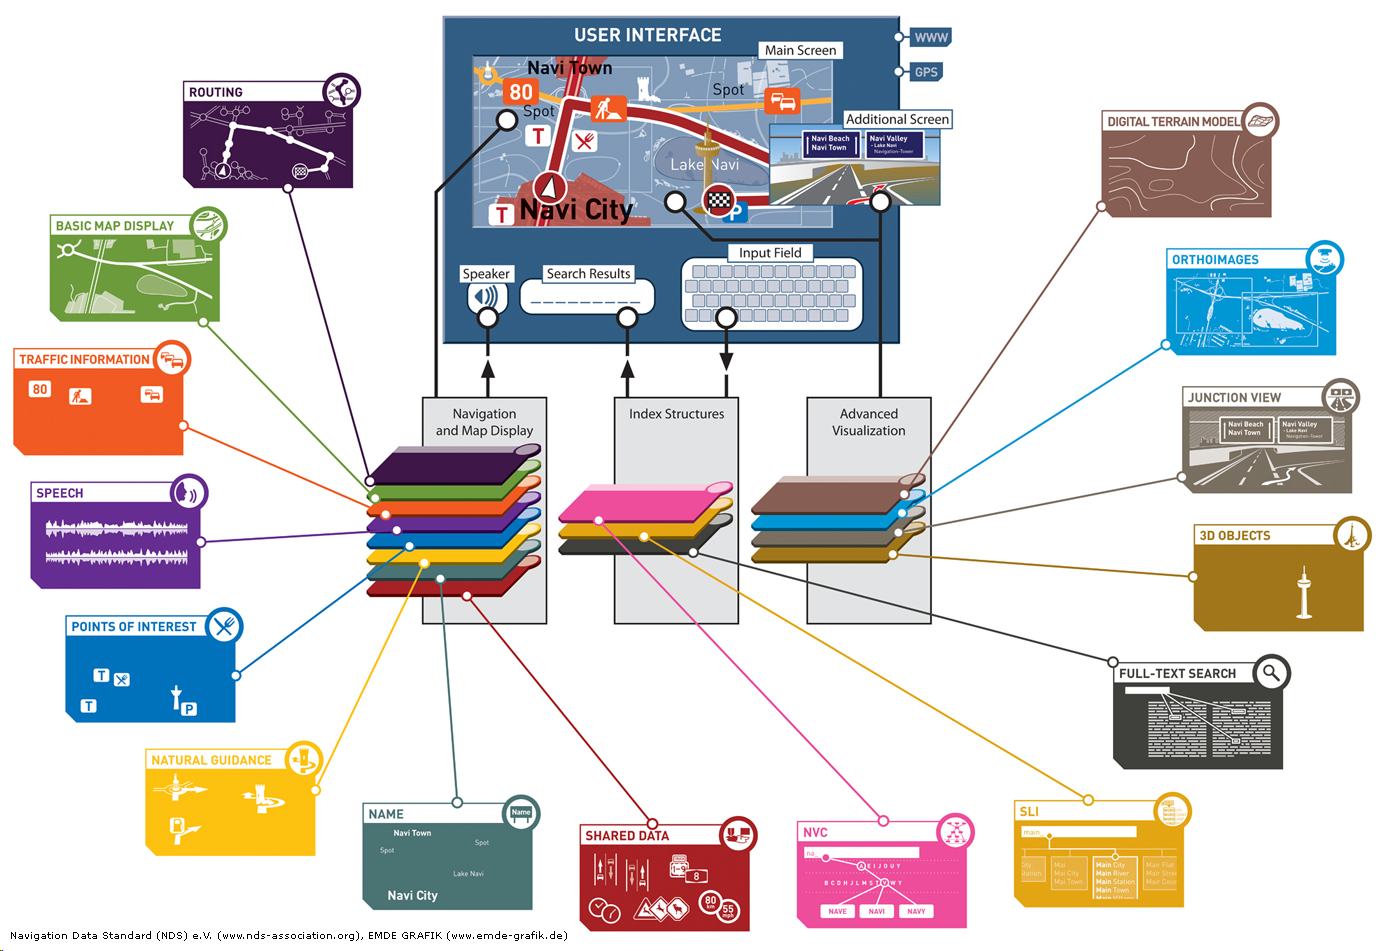
\includegraphics[scale=.42, angle=90]{ndsblocks.png}
\label{fg:ndsblocks}
\caption{Overview of different NDS blocks, source NDS-Specification$\cite{ndsblocks}$.}
\end{figure}


Now, we briefly explain how Navigation Data Standard works in a real-life scenario. Consider two navigation devices fitted inside a car, one of them is NDS-compliant and the other one is not. For simplicity, let's consider device A as non-compliant and device B as NDS-compliant navigation device. Imagine that the region the car is passing through, has been updated. The map providers for device A \& B have generated the newly added changes to the map and they control the delivery process. For device A, the user would have to download the complete compressed binary format of the whole map with new changes. The update process might involve connecting the device to a computer or updating the device using an external storage typically in terms of a USB storage or SD card. For a NDS-compliant device such as device B in this case, the update process is more simple. The NDS format supports incremental updates, the update file size for device B would be relatively smaller that for device A. This in-turn enables such update to be delivered over a cellular connection. Additionally, the update process also takes relatively less time as only the incremental update has to be applied. In case of device A, the whole binary storage had to be over-written. \\

The Navigation Data Standard (NDS) provides a flexible standard for automotive-grade navigation databases. It has been designed to support high-definition maps as well and the incremental updates allow easy updating of different features. 

\section{Updating Map Tile by Tile}
We discussed in earlier in this chapter, how one of the typical approaches is to provide update for the complete geographical region in a large map update. The geographical regions typically are a state of a large country or sometimes even whole country. While this remains a popular choice in current navigation systems in use, it is not efficient to support frequent updates which may arise from high-definition maps. To overcome such a large update size, a patent by \citet{fischer2012technique} describes a technique to support incremental data updates. Their work re-imagines navigation database stored in a navigation system using a novel approach. In their design, they have separated navigation data into at least two layers. They have also suggested that more layers could be added to achieve smaller regions on which an update could be applied. \\

The Navigation Data Standard as explained in Section \ref{nds} simplifies the process of provisioning and updating of the navigation data from multiple map suppliers or navigation systems suppliers or even car manufacturers. \citet{fischer2012technique}'s work is built upon Navigation Data Standard (NDS). However, they have clearly specified that their scheme could also be replicated over a non-NDS navigation database. Their work imagines local tiles which represent local territorial areas with the aim of dividing larger geographical regions such as states, countries etc. which are provided by a navigation database. The size of such local tiles is chosen in such a way that the navigation elements inside the tiles can be easily managed. A very large tile would make many navigation elements linked on one single tile, which might not be ideal. A very small tile can however, limit the amount of navigation elements linked to it. And managing such a large amount of tiles will induce overhead caused by the processing of large number of tiles and their identification in the system. \\

As stated in the first paragraph, \citet{fischer2012technique}'s work structures at least two separate hierarchical layers in the map data. This is done by adding additional information such a road functional class to the already existing navigation database. Each type of road is assigned one particular road functional class. Such functional classes could be grouped together to form the required number of hierarchical levels. For example, for two hierarchical levels, the longer routes such as highways and the state roads could be linked at first level of such hierarchy while the other remaining roads are linked to the second and further level. Their work also proposes to split routes of road segments which span over multiple tiles at first hierarchical level into clusters. Information about such a cluster is stored in the database, so that while updating, they could be interlinked. Interlinking information is crucial to keep the database and road links consistent. The work suggests to identify each road link/road segment if it is not already identified by a unique identifier. These identifiers can be permanent or temporary. However, the tile knot which links related routes at two levels, should have a permanent identifier. Points of Interest (POI) data is kept separate from navigation data so as to allow separate update process for it. Each local tile should also have a unique identifier and maintain its own version data. They also clarify that their design can also work on a navigation database which is designed to support the previously discussed architecture for database. However, NDS already does that. NDS allows each tile to be individually updated. Their main contribution lies in the specialized interlinking of updates between the two hierarchies and the method to identify and process such interlinking. Additionally, their work's novelty could also be found in the method to keep the database consistent by tracking effectively the interlinking between tiles at one level and recursively updating the interlinked tiles while keeping the other structures unaffected.     

\section{Change Detection and Notification}
Previously in Section \ref{actmapprojectsection}, \ref{calcmu}, \ref{maus} and \ref{nds}, we discussed different approaches to apply map updates to a map database. We saw that to save data, individual map data elements should be identified across different versions by their unique ID. This approach can result in significant savings as only the changed attributes are included in the map updates. Now, we will look at \citet{zavoli2008method}'s work to identify these map changes across different versions of map data. In their patent, \citet{zavoli2008method} designed a system which can be used to generate change notifications and deliver map updates to the vehicles based on crowd-sourcing. Their approach utilizes data gathering from multiple vehicles and compares it with the locally available data in the vehicle's navigation system. Their system does not collect position data but other measures such as speed, slope etc to provide better understanding of the current traffic situation. After collecting a significant amount of data about a road segment from multiple vehicles, a central map server compares the collected data with its personal map information available with it in the form of a spatial database. The central server decides upon the significance of the change. If the change is significant based on number of the vehicles reporting it, an alert and update packet is generated. However, if insignificant the central server does nothing. \\

The work inspired us to design a system which could identify what is significant and what is not for a map update, however we use use a different approach to calculate significance. However, their work primarily focuses on crowd-sourcing the data from multiple cars and centrally processing them to select the significance of the data collected. The notable points of their research is generating of change alert and changes by a geographic information server to deliver those updates. Their patent, however is more inclined about collecting new changes detected by vehicles and generating a change based on a substantial amount of collection of newer data. This collection could in-fact increase the bandwidth used by a navigation system used in the vehicle. Additionally, the probe data is dependent on the version of the local geographic database. So based on the version of the locally available map data in a navigation system, it is possible that a vehicle collects probe data while traveling on a road segment as it had older version of map data while another vehicle with updated map data ignores it because it has already received an update about the same road segment earlier.

%\section{An ideal approach}

%\subsection{Why an ideal approach is not feasible}
%While the savings for an ideal approach would be too large, it is highly unpractical for navigation systems. The main reason for not using an ideal approach is the fact that the elements (roads, crossings etc.) within the database are highly interlinked. Replacement/update 


\section{Inefficiencies with Existing Approaches}
While it is clear from work of \citet{min2008mobile}, \citet{cooper2001incremental}, \citet{asahara2008locally}, the ActMAP project\cite{flament2003actmap}, \citet{fischer2012technique} that the concept of differential map updates is the way to go for the future in terms of saving bandwidth while updating navigation/map data. However, their approaches still present some inefficiencies which we see as opportunity to reduce the update size further. The region based updating approach of \citet{asahara2008locally}, \citet{min2008mobile} and \citet{fischer2012technique} only consider the area in question. This could be either preset by the user or could depend upon the subscription previously set by user. Only in the approach by \citet{min2011system}, a protocol is defined which takes the region and its version as input to provide differential updates. In the ActMAP project \cite{flament2003actmap}, the idea is to update all the tiles which will be crossed by the car. In the paper by \citet{bastiaensen2003actmap}, their evaluation describes a scenario where only a map for a city is updated while driving through it regardless of the relevance of such map updates. Their works present different approaches to minimize the size of the map updates delivered to the car, while yet delivering it without any consideration of the relevance of these map updates for the driving car. We want to close this gap by considering the relevance of map updates. We build over these existing yet inspiring work and present our approach in next chapter.     


\chapter{Our Approach}\label{ch:approach}
In the previous chapter, we extensively discussed different approaches \cite{min2008mobile}, \cite{cooper2001incremental}, \cite{asahara2008locally}, \cite{flament2003actmap}, \cite{fischer2012technique} which have been published. After analyzing their approaches carefully, we realized these approaches are effective. Consequently, we believe that in future, such approaches would increase the cost of an autonomous vehicle as more updates would be constantly generated and required. Another thing we noticed with the requirement for autonomous vehicles is that, they already know the location they are supposed to drive to. For human drivers, it is not always necessary to use the navigation system for guidance. For example, when a user is driving to a nearby store in which he/she has already been there, it is not necessary to use the navigation system for guidance. Also, when people are driving in their neighborhood, they rarely use the navigation system for guidance. By having the information about the destination, an autonomous vehicle can choose the optimal path based on current the current situation along the path. For example, the navigation systems are designed to prefer highways over city roads for destinations which are far away. Conversely, due to slow moving traffic on a highway, this could not be optimal. For example, in case of Germany an optimal path which might be longer, could exist using \textit{Bundesstra{\ss}e} instead of the \textit{Autobahn}. \\

The various map updates approaches discussed in Chapter \ref{ch:relatedwork} do not consider such contextual information while providing map updates. Their approaches were targeted more towards minimizing the update by only providing updates for the grids/regions which have changed. The contextual information about an autonomous car's path has not been considered in the previous approaches. However, as we discussed earlier in Section \ref{motivation} for a high-definition map, it would be very expensive in terms of bandwidth to download complete map data over the cellular network. Additionally, such contextual information about the destination can also be used to minimize the update size of any incremental map update. In Section \ref{classificationofupdates} such classification of updates based on relevance to the current route of an autonomous car is explained. We designed a protocol for interaction between an autonomous car and a map update server, which we explain in Section \ref{protocol}.

\section{Classification of Updates} \label{classificationofupdates}
For an autonomous car, it is essential to know its destination. It can be a location hundred kilometers away or a bakery few kilometers away. Nevertheless, it always knows the destination, it is supposed to drive to. Using this information and combining it with the map updates along with other updates such as the weather condition and the current traffic situation, we optimally decide a route for the autonomous car to take. Based on such information, instead of providing updates for all the different grids which have changed, we have an opportunity to derive which updates are relevant and which are not. Using our approach, we now close the gap by classifying updates as relevant/mandatory for the current trip of the autonomous car or not. By using such classification, we further reduce the bandwidth required by the car to receive a constant stream of map updates. By categorizing map updates into contextually relevant or mandatory updates and the remaining as optional updates, the data requirements are reduced. \\

\begin{figure}
\centering
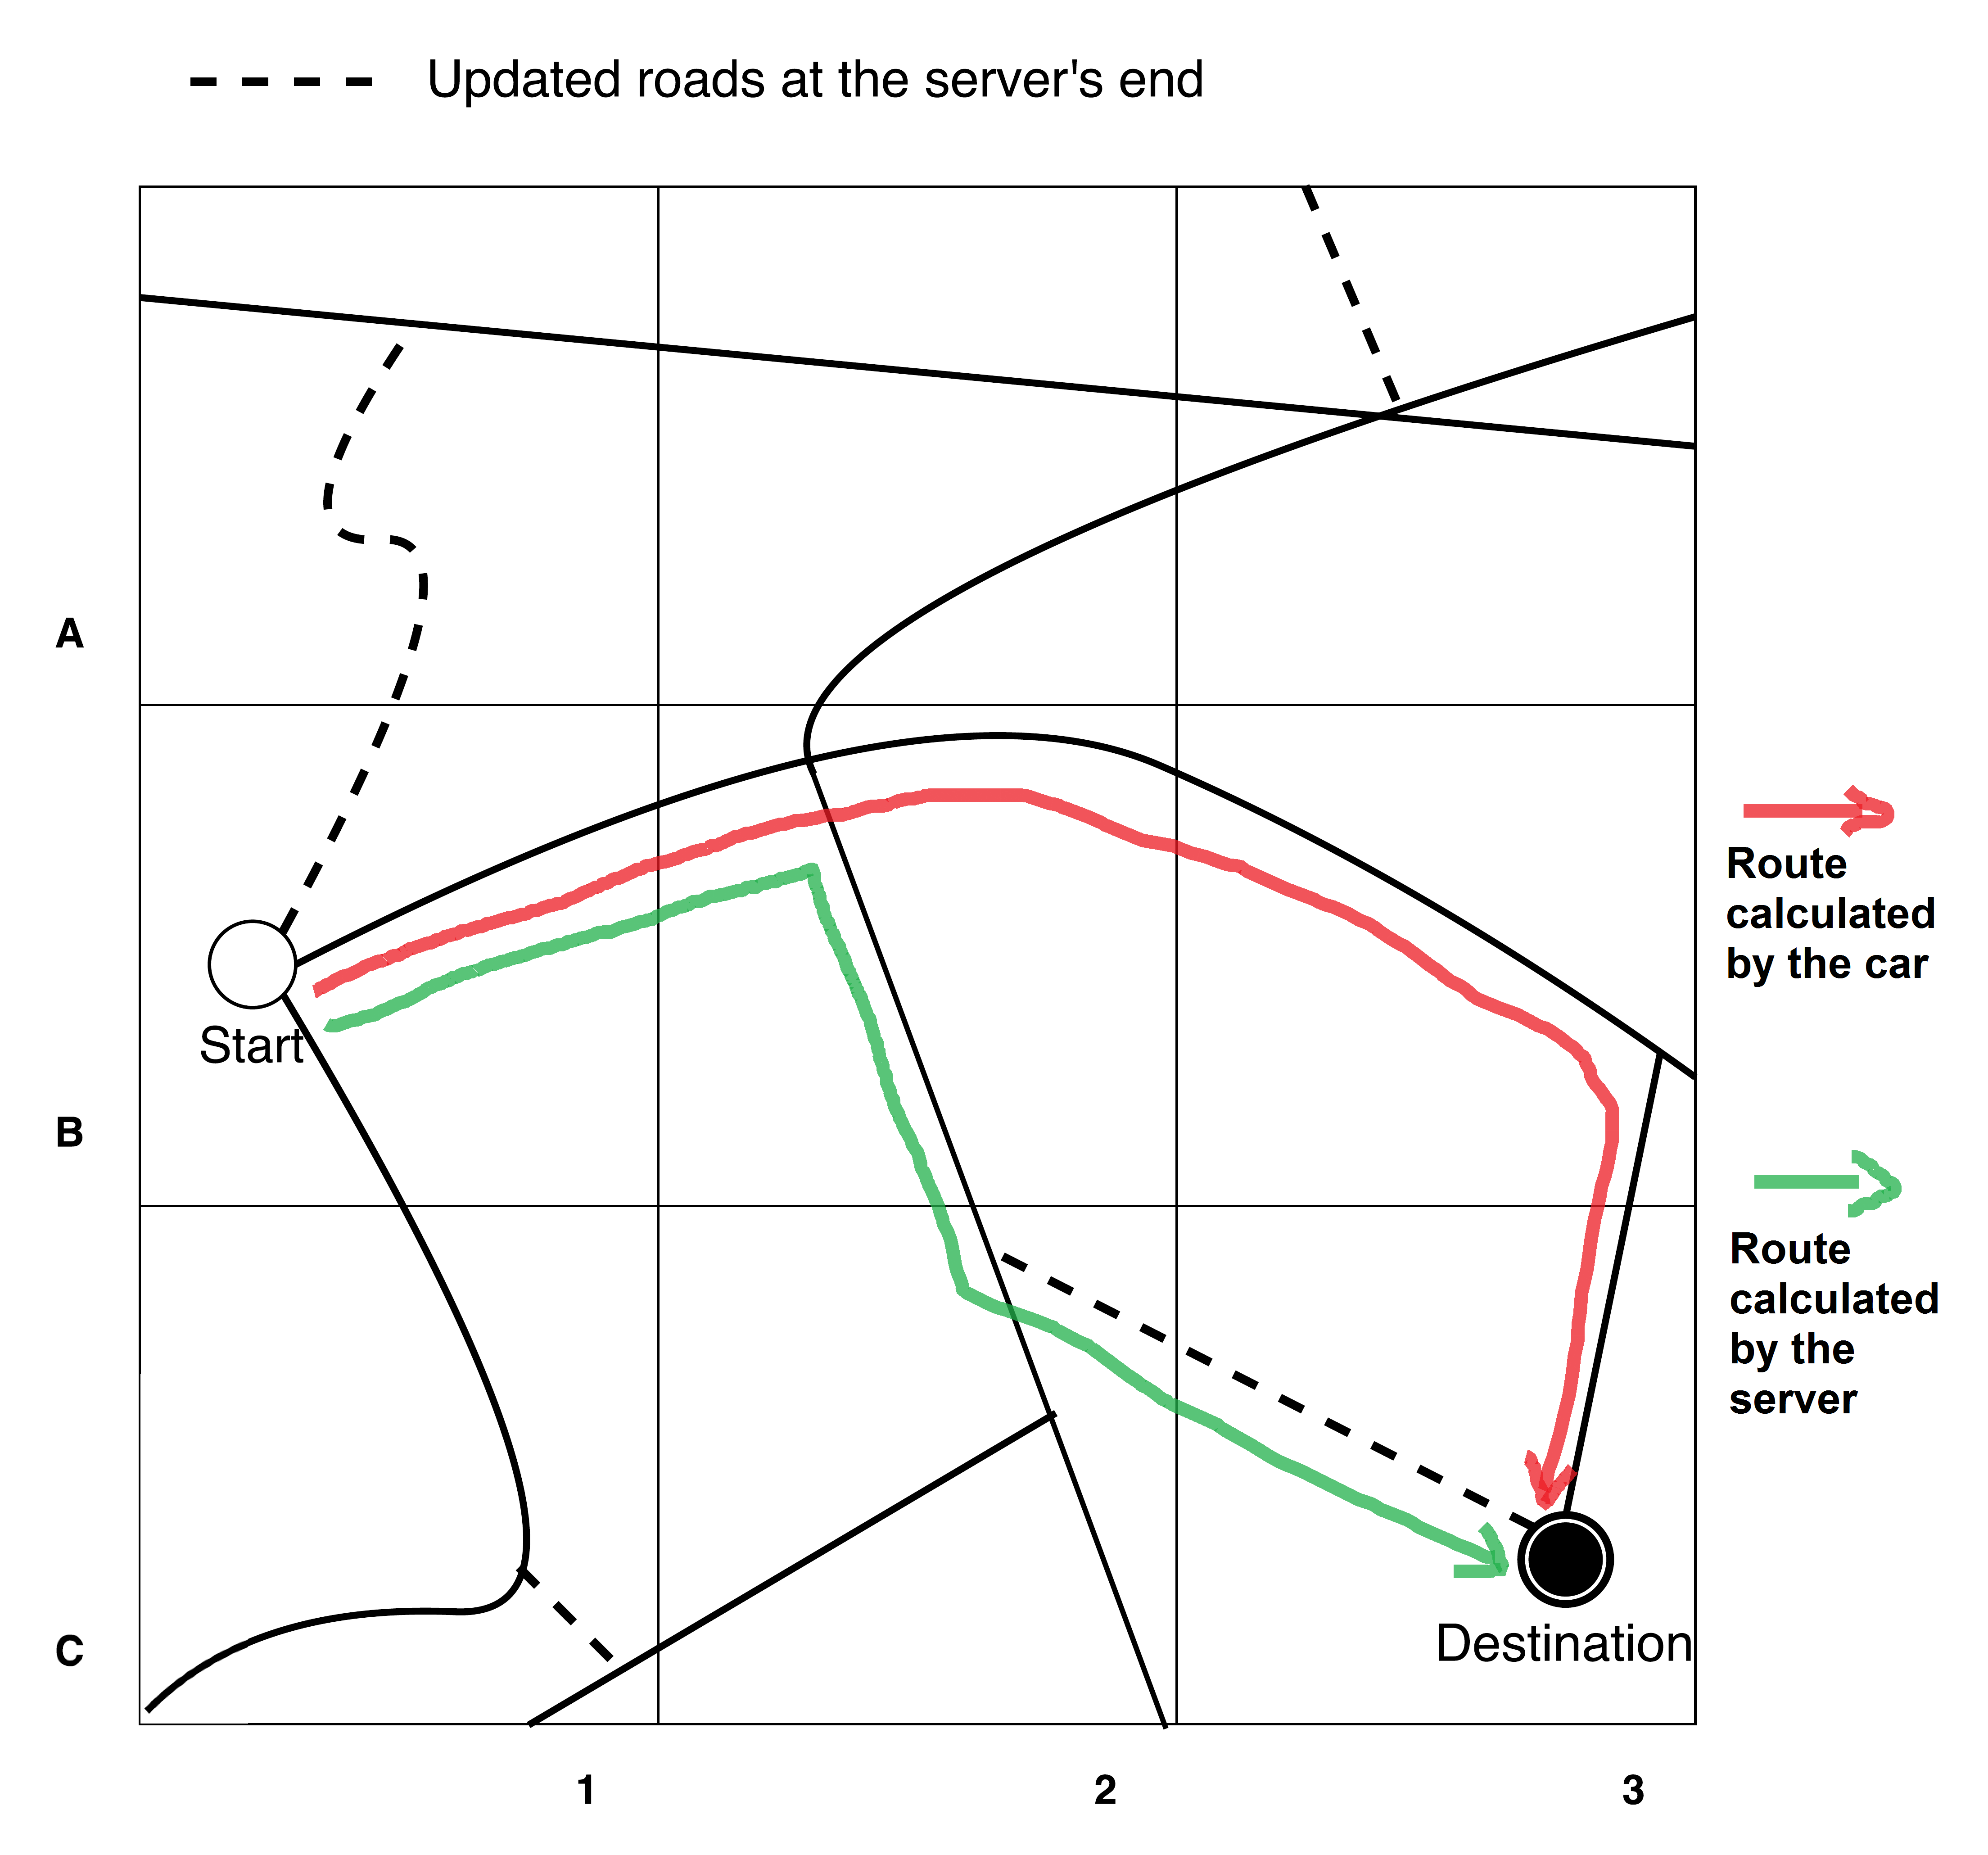
\includegraphics[scale=.12]{classification6.png}
\caption{General working principle behind the classification of updates.}
\label{fg:classificationofmapupdate}
\end{figure}

With the help of an example, we now present our approach on classifying grid level updates as mandatory or optional. In Figure \ref{fg:classificationofmapupdate}, assume that the autonomous car starts at the location marked "Start" and has the destination marked as "Destination". The road network is divided into multiple layers from level 1..n, level 1 being most important roads such as national highways down to level n for residential streets (Section \ref{maus}). We have used different classification for such roads which has been explained in Section \ref{gridsizeclassification}. For simplicity, we are considering that all the roads shown in the figure are of one type only. The dark, bold lines indicate the route which exists locally stored in the navigation system of the car. The dotted lines represent the newly added roads in that area. However, these changes have not been delivered as updates to the autonomous car. The grids are marked A to C vertically and 1,2 and 3 horizontally. The grids could be referred as A1, A2 and A3 in first row \& A1, B1, C1 in first column and so on. Grids A1, A3, B1, C1, C2 and C3 have been updated at the server's end. However, this information is not yet available at the car's end. We would now discuss how our approach classifies some of these grids as mandatory or optional.
\subsection{Mandatory Changes}
In our example, based on the map information car has locally, it chooses the path going through grids B1, B2, B3 and C3 (marked in red) to arrive at the destination. However, based on the updated information at the map server's end, it calculates the optimum path using grids B1, B2, C2 and C3 (marked in green). Using the routing information and seeing the changes we have on the map, only the updated information in grids C2 and C3 is necessary for the autonomous car to arrive at the destination using the optimal path calculated by the server based on current state of map data. 
\subsection{Optional Changes}
Unlike the grids C2 and C3, the changes in other grids do not necessarily affect the optimal routing to reach destination. The changes in grid A1, A3, B1 and C1, even if they are downloaded and applied in the car's navigation system along with map updates of grids C2 and C3, does not affect the optimal route calculation to destination. The downloading of map updates for other grids, which indicate changes (A1, A3, B1 and C1) could be deferred. 
\subsubsection{Deferring Optional Updates}
Based on the simple example in Figure \ref{fg:classificationofmapupdate}, we explained how we can classify grids which have updates into mandatory and optional, based on the contextual information about the destination and optimal route calculation. Such a route calculation also depends on the map data a car has locally. In our example, we saw that map updates for the grids A1, A3, B1 and C1 could be marked optional since they did not affect the current route calculation to reach the destination. Such updates could be marked and deferred to be downloaded later when the cost of bandwidth is high. Such approaches have been presented in work of \citet{balasubramanian2010augmenting} where the less-critical data is deferred to be downloaded over WiFi. By applying such principles of tagging map update grids as mandatory or optional, it is possible to download and apply only mandatory map updates by the car online specifically requesting for those updates similar to approach described by \citet{min2011system} in their work. \\

In order to achieve sufficient savings, such optional map updates should be deferred until they become mandatory. One approach could be to download these updates depending on when the cost of bandwidth is low. This could be the result of a WiFi based connection from a public hotspot or at home or garage of the car's user where a WiFi connection is available. Additionally, such optional updates could be transferred between cars using vehicle-to-vehicle communication which is beyond the scope of this thesis. We have mentioned the idea of such strategies in the future work (Section \ref{futurebfs}).
\section{Grid-size Classification} \label{gridsizeclassification}
Through our example in Section \ref{classificationofupdates}, we looked at how we can classify grids with changes into mandatory or optional. However, the optimum grid size is also a deciding factor regarding the amount of data which has to be transmitted for map updates. Also, while applying these updates we have to consider the inconsistencies induced in the map data as well. We could use the approach similar to \citet{asahara2008locally}, which checks for nearby grids which have connections from the grid which is being updated. However, a grid size would play an important role. A relatively larger grid would deliver larger update consisting of many changes and will reduce overhead in the calculation of whether it is mandatory or not. However, it will also add contextually irrelevant map object updates, similar to the existing approaches by \cite{min2011system} and \cite{bastiaensen2003actmap}. \\

Modern routing algorithms divide the amount of the streets into different subcategories, accordingly to their type. This hierarchical layering enhances the overall performance of the route calculation process as described by \citet{min2011system}. As one of the contributions of the Dynamic Map Update Protocol we adapted and modified this concept for routing algorithms for the use case of map updates. The division of different road types is performed as a pre-processing step on the map database. The different street types can be categorized into different categories. However, for the implementation, the street types are clustered into two different map layers. One layer contains all highways. The other layer the remaining streets, e.g. city streets. Each of the two layers is then divided into map tiles of different size (see Figures \ref{fg:diffroads} and \ref{fg:geohash}). This is done due to the different available speed limits. The highway layer map tiles are larger than the city street map tiles, as the vehicles can drive further on them in less time. Highways are therefore prioritized over city streets by the routing algorithms when the car has to go further distance. This design decision helps to reduce the amount of control traffic, which has to be conducted in the process of the protocol when requesting further map tiles. When calculating its new route the highly automated car receives then only the map tile updates required for the currently used layer. A highly automated car driving over a highway for example, is not interested in the city streets of a town nearby if it never goes through the town on it's trip. It will therefore only get updates regarding the highway, but not the city streets layer in this area. As shown by \citet{fischer2012technique} in their work, multiple categories can be used for classifying roads into different categories of different map grid sizes. However, for simplicity we used only two separate classes of roads. In our work, we have separated highways and all other related roads into two categories. Based on OpenStreetMap's classification, we identify \textbf{highway} as the roads of the following class
\begin{itemize}
\item "motorway"
\item "motorway{\_}link"
\item "motorway{\_}junction"
\item "trunk"
\item "trunk{\_}link"
\item "primary"
\item "primary{\_}link"
\item "secondary"
\item {secondary{\_}link"
\item "tertiary"
\item "tertiary{\_}link"
}\end{itemize}

and we identify \textbf{city roads} as the roads of following class
\begin{itemize}
\item "road"
\item "residential"
\item "living{\_}street"
\item "service"
\item "unclassified"
\end{itemize} 


These classes are read from OpenStreetMap data which has been explained in Section \ref{osmattributes}. Based on this classification, we have realized grids of two different sizes. Even though multiple levels of grid sizes can be used, we have limited our implementation to use only two separate levels. The relatively larger grid is used for \textit{highway} class roads. Another relatively smaller grid is used for \textit{city roads} in our implementation (Section \ref{ch:implementation}). Section \ref{geohashsizes} explains the map grid sizes in details used in our implementation. Figure \ref{fg:diffroads} shows an example of such classification in the city center of Berlin. The thick dotted lines in the figure indicate the streets belonging to the class \textit{highway}. The remaining thinner lines indicate streets belonging to the class \textit{city roads}. 


\begin{figure}
\centering
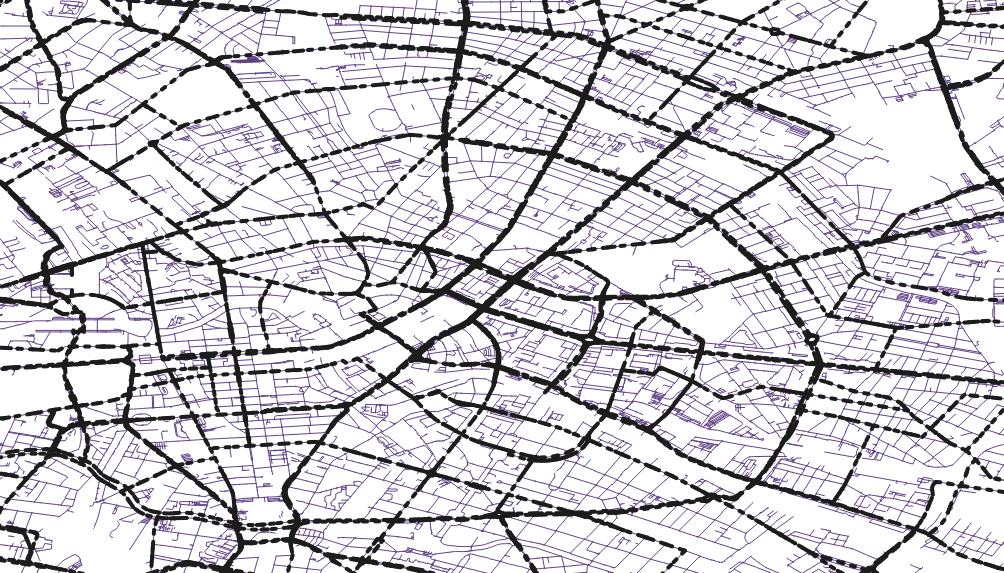
\includegraphics[scale=.65]{berlincity.png}
\caption{Division of streets of Berlin city center into two classes, highway marked by thick lines and city roads by thin lines, {\copyright} OpenStreetMap contributors. }
\label{fg:diffroads}
\end{figure}  



\subsection{Geohash}\label{geohashsizes}
\begin{figure}
%\centering
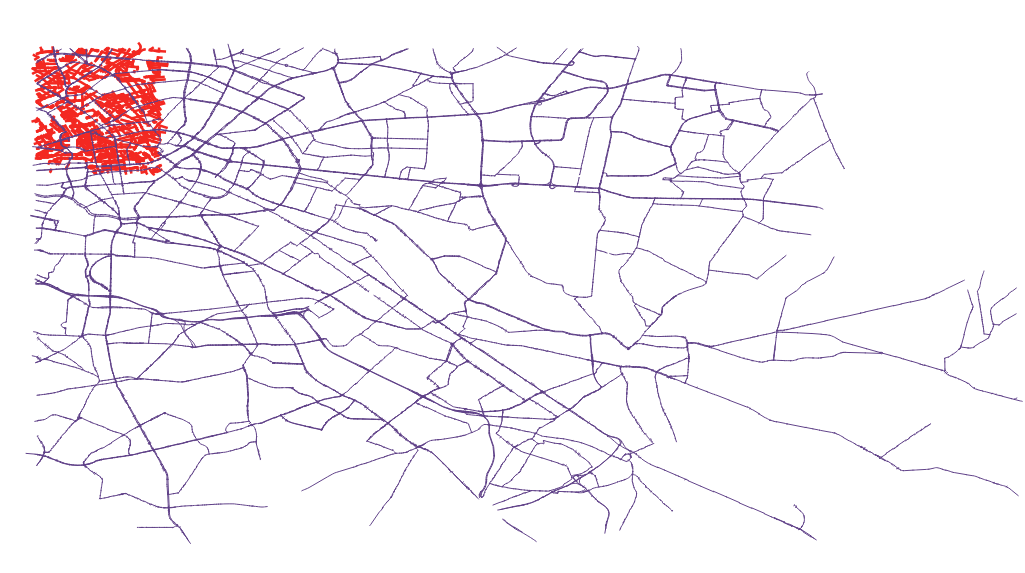
\includegraphics[scale=.65]{geohash2.png}
\caption{Size of a city road layer grid (marked in bold) in comparison to a highway grid in Berlin city, {\copyright} OpenStreetMap contributors.}
\label{fg:geohash}
\end{figure}
As discussed in Section \ref{gridsizeclassification}, dividing a map into specific grids is an important step for minimizing the update size for the map. However, we required a universal grid identifier system using which we impose different grid sizes suiting to our needs. That is where Geohashes come into picture. For the identification of a specific map tile, we use the indexing structure provided by the concept of Geohashes (\citet{suwardi2015geohash}). A Geohash is a unique string that identifies a certain geographic area on the Globus. Each Geohash identifies its personal rectangular bounding box. Neighbouring geographic areas just differ in the last letter of the Geohash. By adding up further letters to the end of the Geohash the area of the bounding box is shrunk accordingly. Geohashes therefore are a well suited indexing structure to satisfy the needs of the Dynamic Map Update Protocol. For the evaluation of the scenario of the city of Berlin in Chapter \ref{ch:evaluation}, we chose the Geohash string length of four letters for our highway street layer and five for the city street layer. These string lengths match on bounding box sizes of 39.1km x 19.5km and 4.89km x 4.89km, as can be seen in Figure \ref{fg:geohash}. The general concept of different map layers can be enhanced further by adding up more fine granular layers if beneficial for future use cases of the Dynamic Map Update Protocol. \\

Precision value '5' is used by city roads, marked in bold in the figure. On the other hand, a Geohash precision value '4' is used for creating grids for highways classified previously in Section \ref{gridsizeclassification}. Despite being relatively larger in size, only the highway class streets are considered in that grid. The separation of these different classes of roads into different sized grids (Section \ref{geohashsizes}) is an important step to deal with the probability of updates. The roads belonging to the highway class, are relatively less likely to change and the larger sized grid is not as dense as the smaller city grids. The denser distribution of city roads is handled by a relatively smaller sized grid to avoid unnecessary updates to different portions of the region. 

\section{Dynamic Map Update Protocol}\label{protocol}
Building upon our concept of identifying mandatory grid updates (see Section \ref{classificationofupdates}), we defined a protocol between a navigation system and a map update server to perform map update using our approach. We call it the Dynamic Map Update Protocol. The protocol aims to ensure that after the delivery of mandatory updates to the navigation system, the requesting vehicle would calculate the same route as the server. Through the protocol, the optional map updates are marked, but not delivered to keep the footprint of transmission costs as low as possible. The different steps of the protocol are illustrated in Figure \ref{fg:protocol} in detail. And will be explained in the following section.


\begin{figure}
\centering
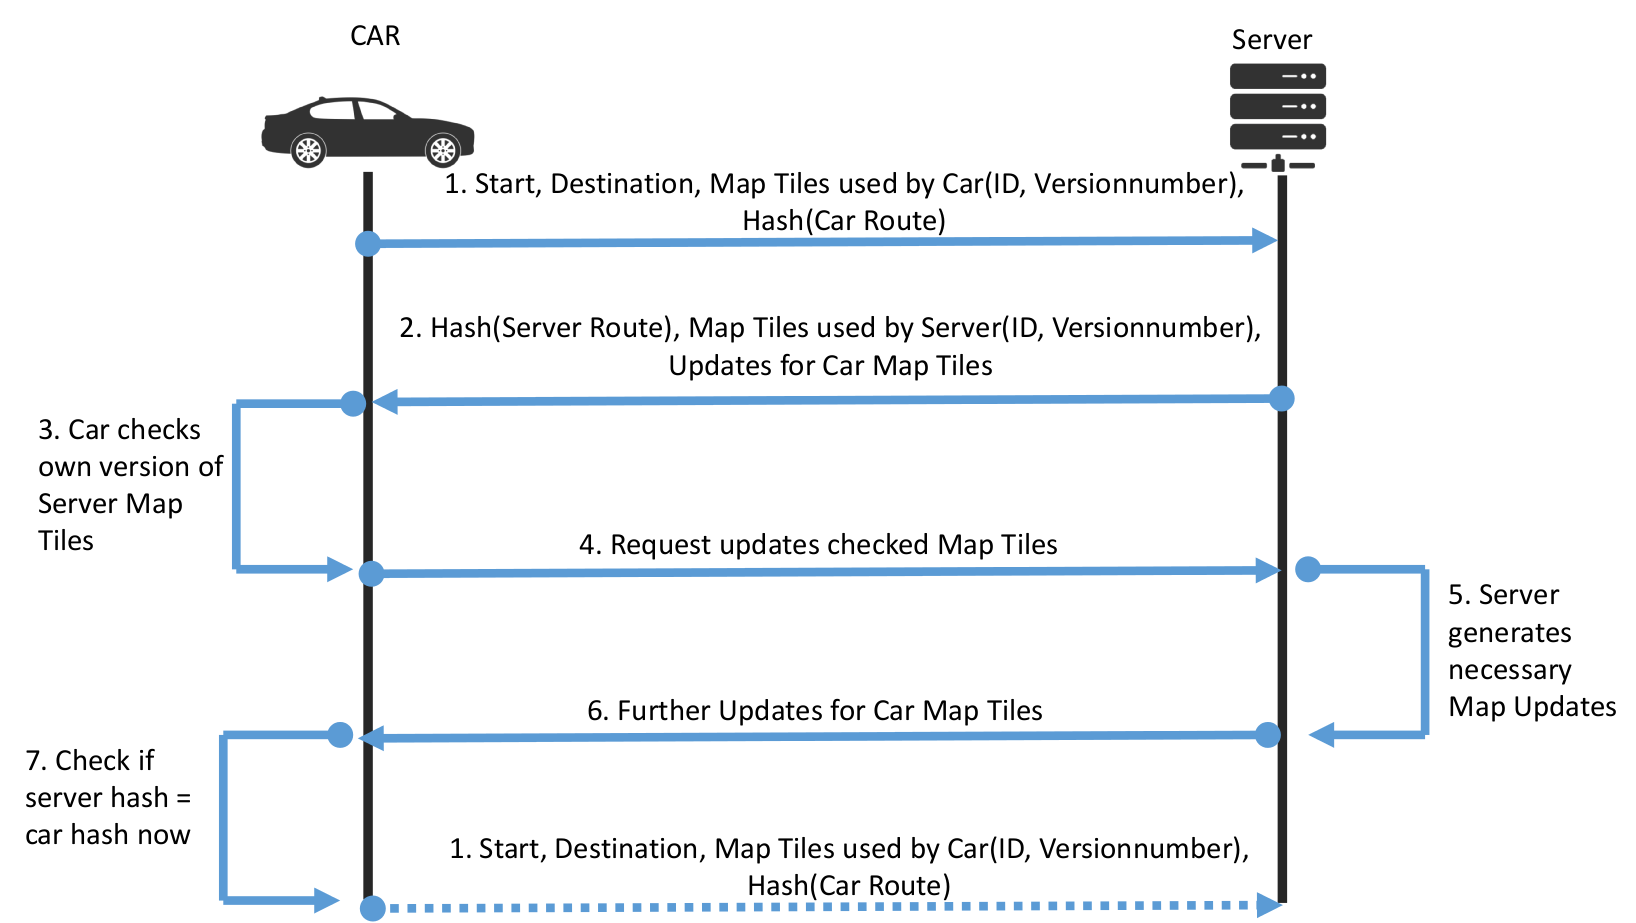
\includegraphics[scale=.32]{dmup.png}
\caption{The Dynamic Map Update Protocol sequence.}
\label{fg:protocol}
\end{figure}



\subsection{Protocol in Detail}
We now look at each step of the protocol illustrated in Figure \ref{fg:protocol} and explain the necessary calculations.
\begin{enumerate}
\item After receiving input about the destination and calculating its current location, the car calculates its route to reach the destination based on its locally available map data. After that, the car requests an update for it's calculated route by providing the server the source and the destination along with some additional details. The additional details include the list of map tiles used for the calculation of the route and the unique hash-code of the route. Providing this list of map tiles is done in a data efficient way. Only the map tile that contains the start point will be specified through a complete identification ID and layer level number. After that, the next map tiles used by the car will be described in relation to their previous map tile. Therefore, only limited information is required, which indicates the possible ways (up, down, left, right with reference from the last tile) in which the vehicle can move and whether the current map layer is changed or not. For each traversed map tile the car will also provide its current local version number it has. Figure 4.5 illustrates this in further detail. The exact route, which the car will use, is identified through a unique hash-code using the road segments. Therefore, each ID of the route segments, that the car has to take on its course, add up as an additional input value to a hash function. After the completion of this process the generated hash-code of the current route is sent to the server as well.

\item Upon receiving the values from the car described in the previous step, the server extracts the start and the destination point. The server will then calculate its own route from the start point to the destination point based on the its up to date map data. The server will also calculate the hash of the route it calculated, using the same hash function used by the car. Upon comparison of its local hash-code with the hash-code it received from the car, the server will be able identify whether the routes are the same or not. If both hash-codes match, it means that at least the current road to drive on is up to date in terms of the server's database. It still might be the case that optional updates for the car are available. These are updates for the specific map tiles the car traverses, which do not belong to the actual road it drives on. In future situations the car could drive in these areas as well. So an update might still be beneficial for the car. Therefore, the server checks the different versions of the traversed map tiles. If they also match, everything is up to date. The server then just replies with a short response, indicating that the map material of the car does not require updates for the route. If optional map updates are available, the server will provide the car the ids of the map tiles, which could receive an update. Based on its driving criteria and other parameters like remaining cellular data volume, the car than can decide if and when it wants to receive those updates later on. If mandatory updates have to be provided, the server directly generates those updates and sends them back to the car. If the servers route uses other map tiles than the car, the server provides its own hash-code and the map tile ids and version numbers used for calculation to it. This step is necessary to ensure that the car does not find another as well outdated alternative route in its own database. 


\begin{figure}
\centering
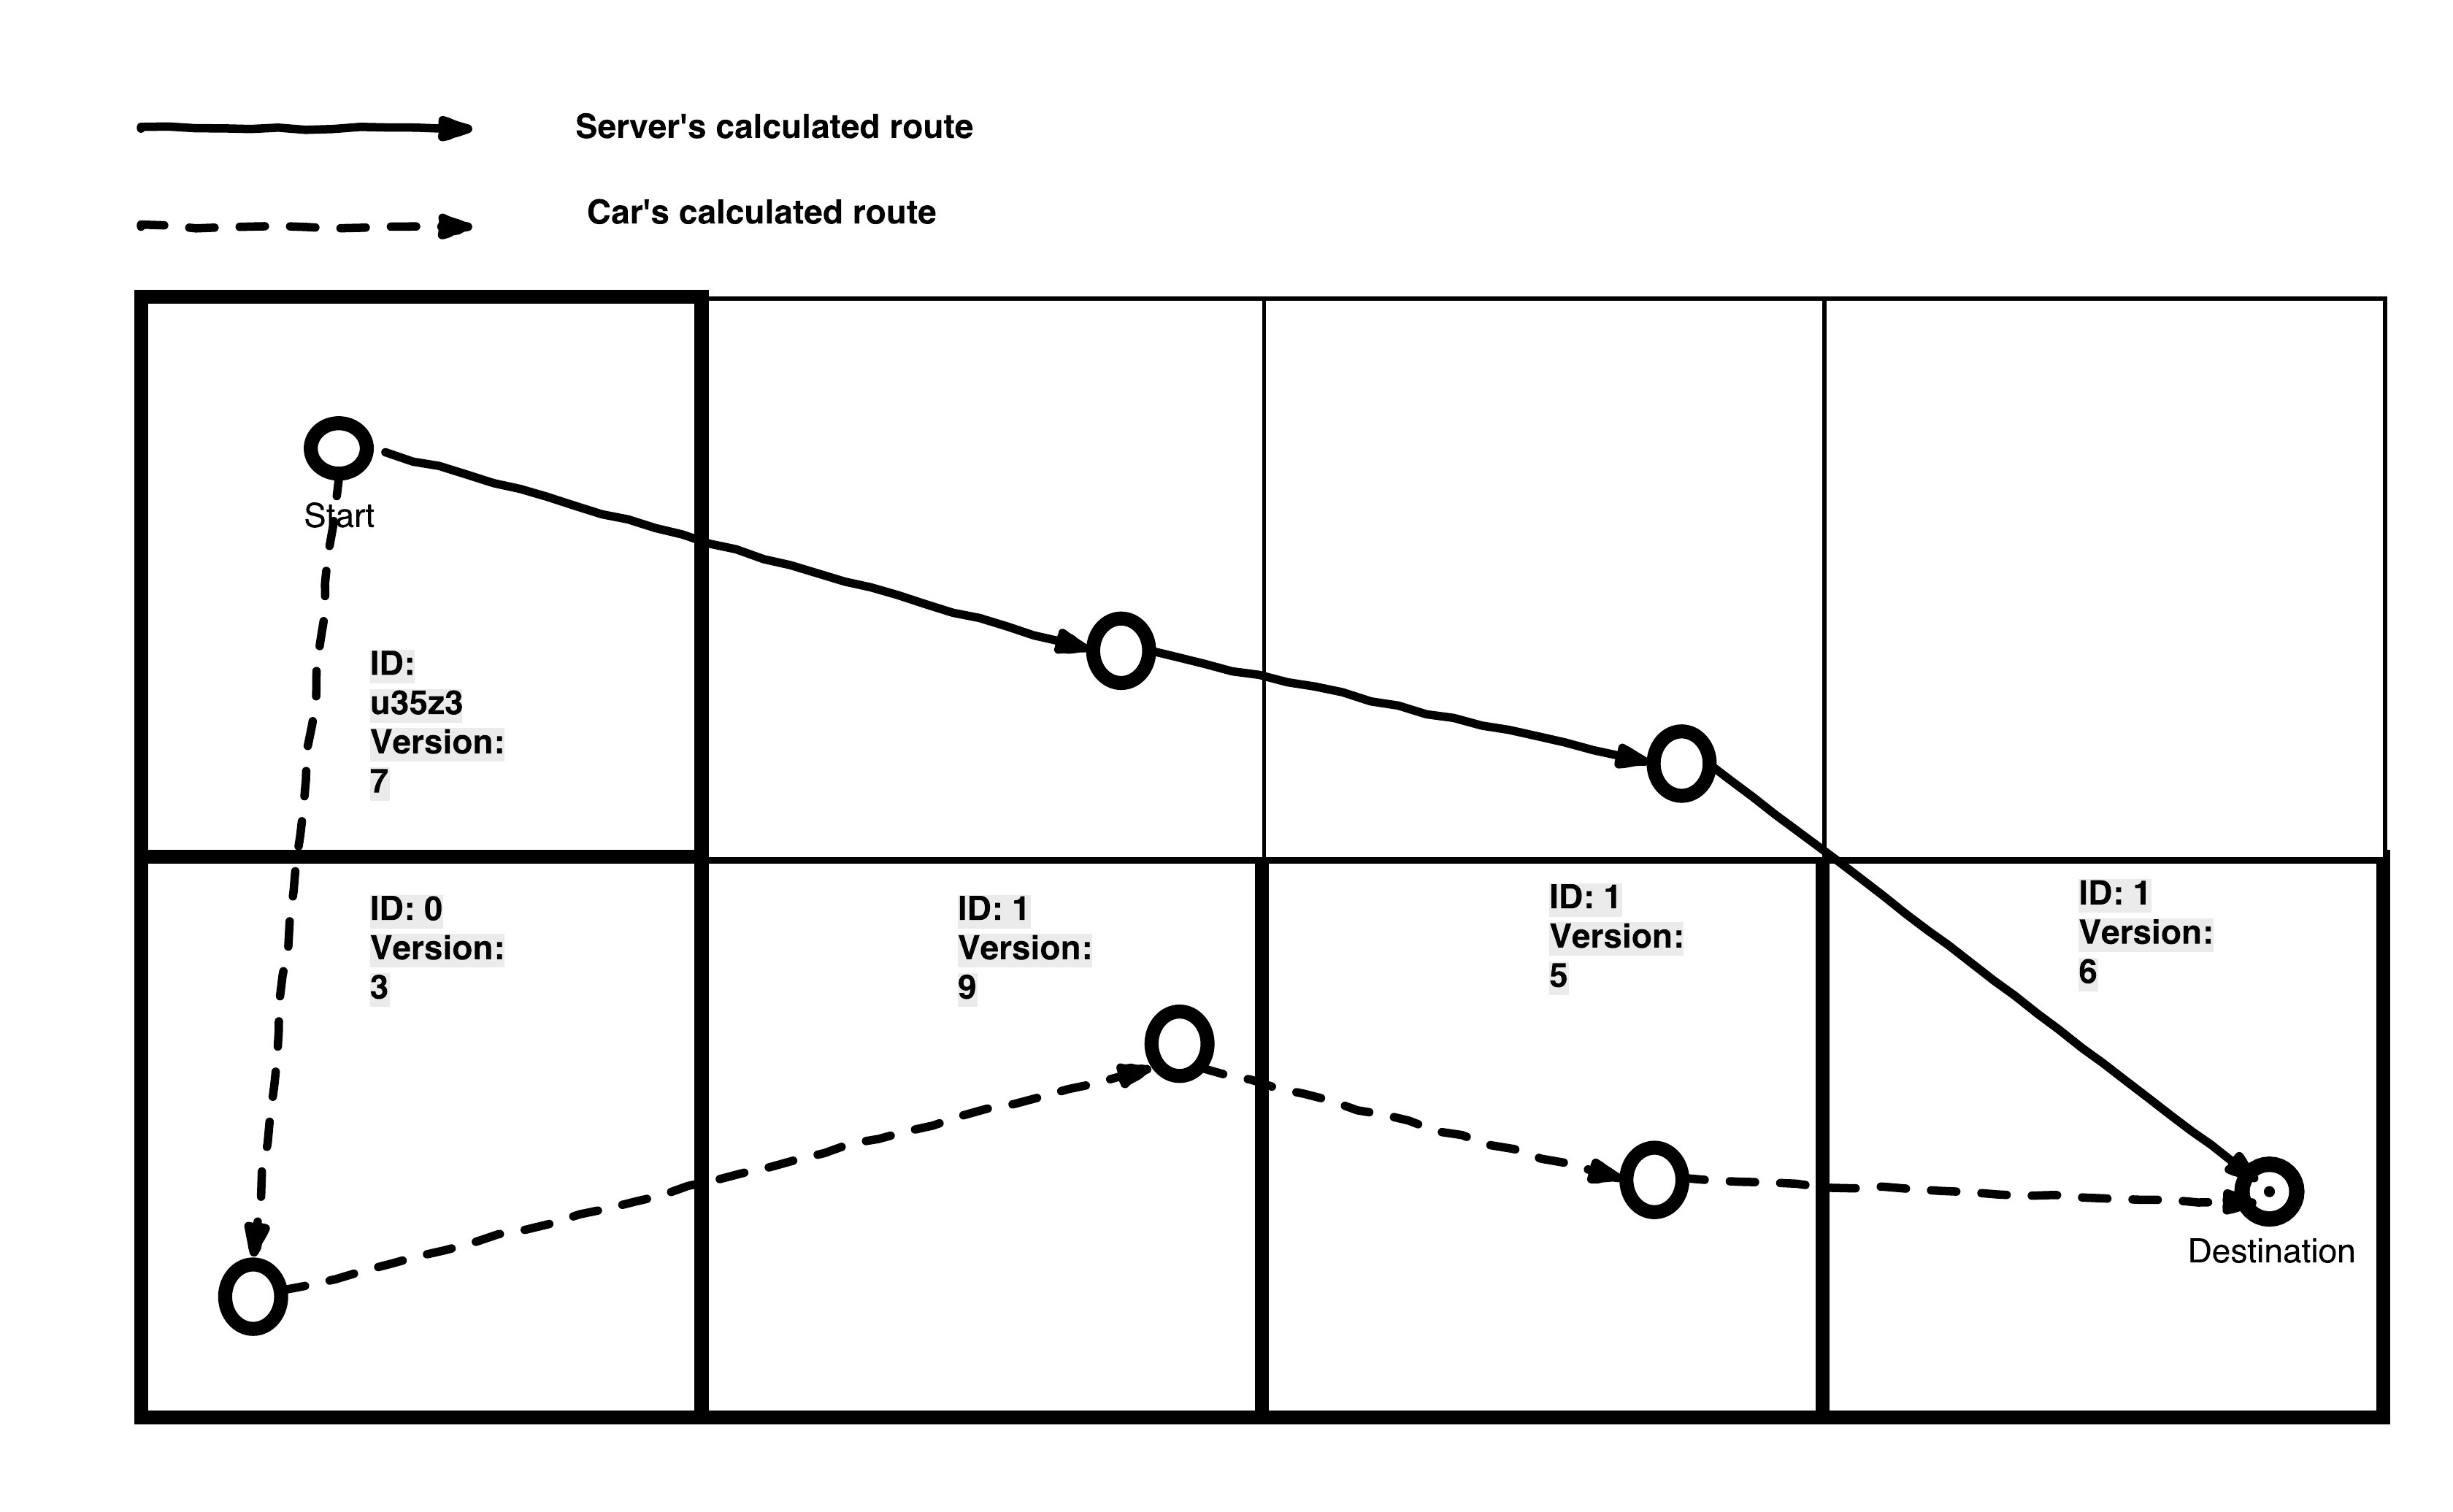
\includegraphics[scale=.18]{gridnumbering.png}
\label{fg:numberingtiles}
\caption{Sequencing method of used map tiles/grids.}
\end{figure}




\item Then the car has to further update its own map database for the newly provided route. Therefore it checks the map tiles indicated by the server in its own database for mandatory map updates. It requests them accordingly and gets them provided by the server.

\item The requested mandatory map tiles update is provided by the server to the car in a single map update object.

\item After applying the mandatory updates, the car recalculates the route from the source to the destination and calculates the hash-code for the route. The car compares the hash-code generated from the new calculated route with the server's hash-code. If it matches, it simply replies to the server with acknowledgement. 

\item In rare occasions the provided map updates might not be enough to ensure an up to date routing capability of the car for its current route. It still might be the case that the car finds a faster, but an outdated alternative route using other map tiles. The protocol has to ensure that the car uses the currently fastest route now and in future calculations. Therefore the car has to check whether now its personal hash code matches with the server's code or not. If it does not, the whole procedure has to be repeated with the new conditions. This however should not happen very often because of the actual size of the map tiles. It makes shorter alternative routes mostly unlikely.



\end{enumerate}


\subsection{Concepts for Map Updates} \label{calcmu}
In Section \ref{protocol}, we described the workings of our Dynamic Map Update Protocol. The protocol calculates the significance of each updated grid and classifies them into two different categories using the requested trip information and the state of map data available at the car's end. Since only the mandatory grids, which are relevant to requested route are provided, it is necessary to discuss what is included in the map updates. In our example of considering the navigation layer of a map data, we have used a similar approach of incremental map updates as suggested previously by the works of the ActMAP project \cite{flament2003actmap} and the locally differential updates of \citet{sakamoto2000proposal}. We also considered \citet{asahara2008locally}'s approach to Connection Maintained - Locally Differential Updates to maintain consistency of the map data. Similar to the approach of \citet{hitachi}, complete updated for mandatory grids could be provided in one set of all the changed objects. This would save in creating a separate request for individual grids as suggested in works of \citet{min2011system}.

\subsection{Newly Added Routes}
A newly developed path or a newly mapped route in the map could be useful to shorten the route between the car and its destination. In such cases, when generating a new update, only the changes in a specific grids are considered as part of the map update object. Similar to \citet{sakamoto2000proposal}'s work, the new routes which have been added in a particular grid become part of the map update object pushed to the navigation system of the car. 
\subsection{Deleted Old Routes}
In some cases, references to an old route are deleted and a new updated route with a new unique identity is mapped by the map makers. Additionally, closure of some roads by city administration or restricting only bicycles on such routes could also lead to such routes being deleted from the navigation map database. Since the map only requires to have details about routes on which an autonomous car can drive, such routes are required to be deleted for optimal path calculation. Using a differential update method for the mandatory grids, such routes could be marked for deletion by passing unique identifiers of such routes in the map update object. 
\subsection{Updated Old Routes}
Although it is highly unlikely that the roads are deleted from the city, it is quite possible that some roads are marked restricted for private transport. Additionally, during festival season or during repair of the road, it is necessary to provide such information to the car. Without such updated information about the streets, accidents could happen which can incur fines as well. To provide such information to an autonomous car, specific route elements with their unique identifiers along with updated parameters could be packaged in a map update object. 
\section{Certain Inefficiencies}
In our approach, the significance of a grid/map tiles is calculated based on the changes it has and how relevant they are for the requested trip path calculation. The grid size is an important factor in deciding how much other non-relevant map updates are provided bundled with the crucial map updates. As presented earlier in Section \ref{grids}, a very precise and small grid size would result in large control flow overhead due to larger identification numbers. And a very large grid size would result in larger more unnecessary map updates, thereby wasting crucial bandwidth in some cases. 
\subsection{Breadth-first Approach}
To overcome the inefficiencies mentioned earlier with the grid based approach, we tried with an approach of finding relevant map objects connected to crucial changes in a breadth-first search manner similar to the approach stated by \citet{hitachi}. For this, instead of comparing map tiles/grids for changes based on version, we tried comparing the individual map objects based on their versions. After the first iteration, we would look for other map objects linked to the crucial map objects as stated by \citet{hitachi} and check if they have changed. If they have changed, we would also add them to the update object. And we continue this in a breadth-first manner. To further develop this approach and evaluate its potential, we conducted a small evaluation of the breadth-first approach over heavily updated areas like the city of Berlin. Figure 4.6 shows results of one such evaluation. In first image, one can see a very small segment of road marked for update as identified by our approach. In 1$^{st}$ iteration, all the roads connected to the previously identified segment which has changed in the newer map is identified and marked. We used the version information associated with each way object in OSM data (see Section \ref{osmattributes}) for deciding whether the road has changed in the newer map data or not. As discussed earlier, the changes can be addition, deletion or update of the road element in map data. In further iterations, as shown in the figure the amount of marked roads for update increased drastically. Once this approach adds a main street in a city to the list of changed objects, the list of connected changed roads, grows at a much faster rate. This can been seen in the iterations 3, 4 and 5. Also, this approach had quite a large overhead for providing each individual map object's version number and was much much slower. OSM Map data does not seem to be fitting for the Hitachi approach. Therefore, we did not investigate it further and have listed it as one of the future work related to this thesis in Chapter \ref{ch:conclusion}.   




\begin{figure}
\centering
\label{fg:bfsberlin}
\subfloat[The relevant changes identified by our algorithm]{ 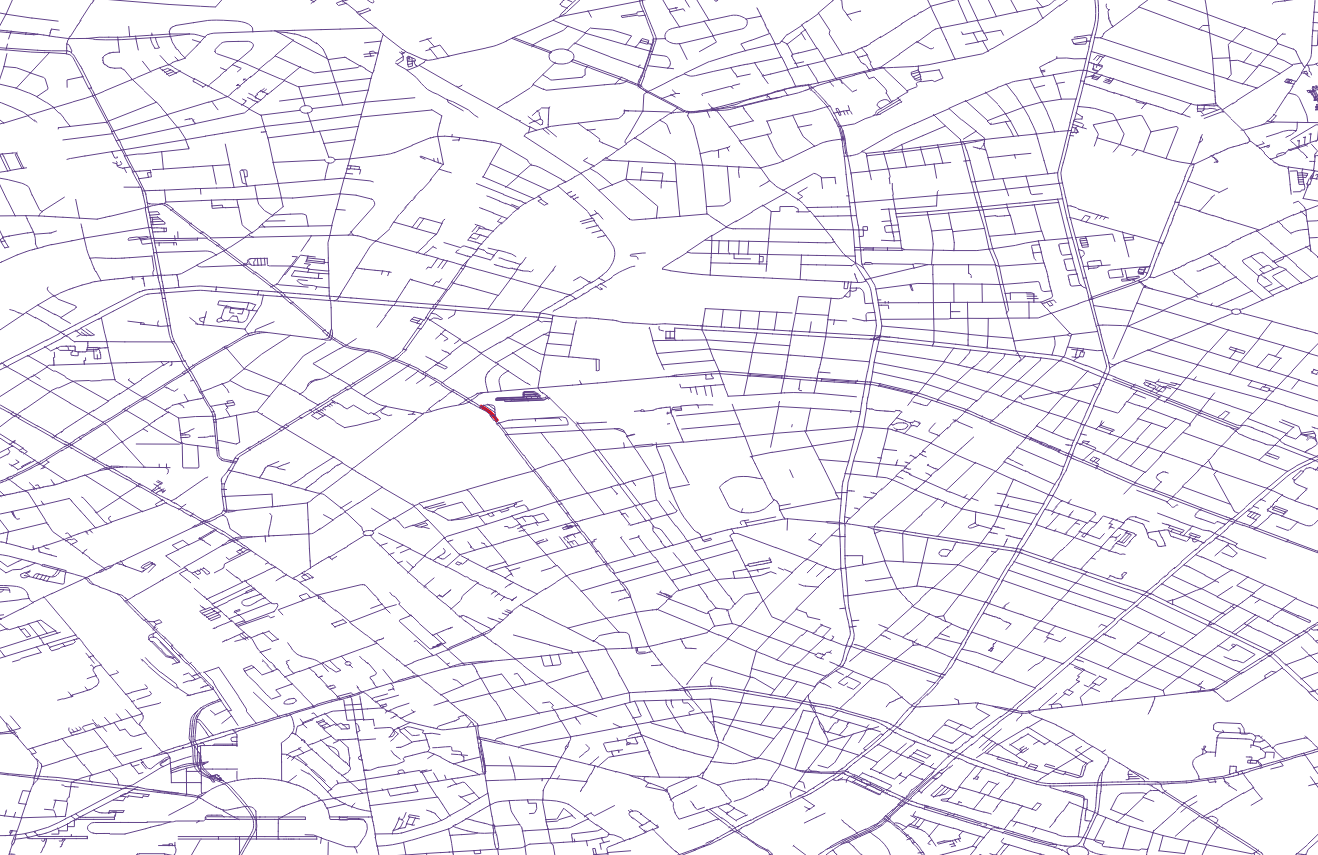
\includegraphics[scale=.25]{1.png}}
\subfloat[After Iteration 1]{ 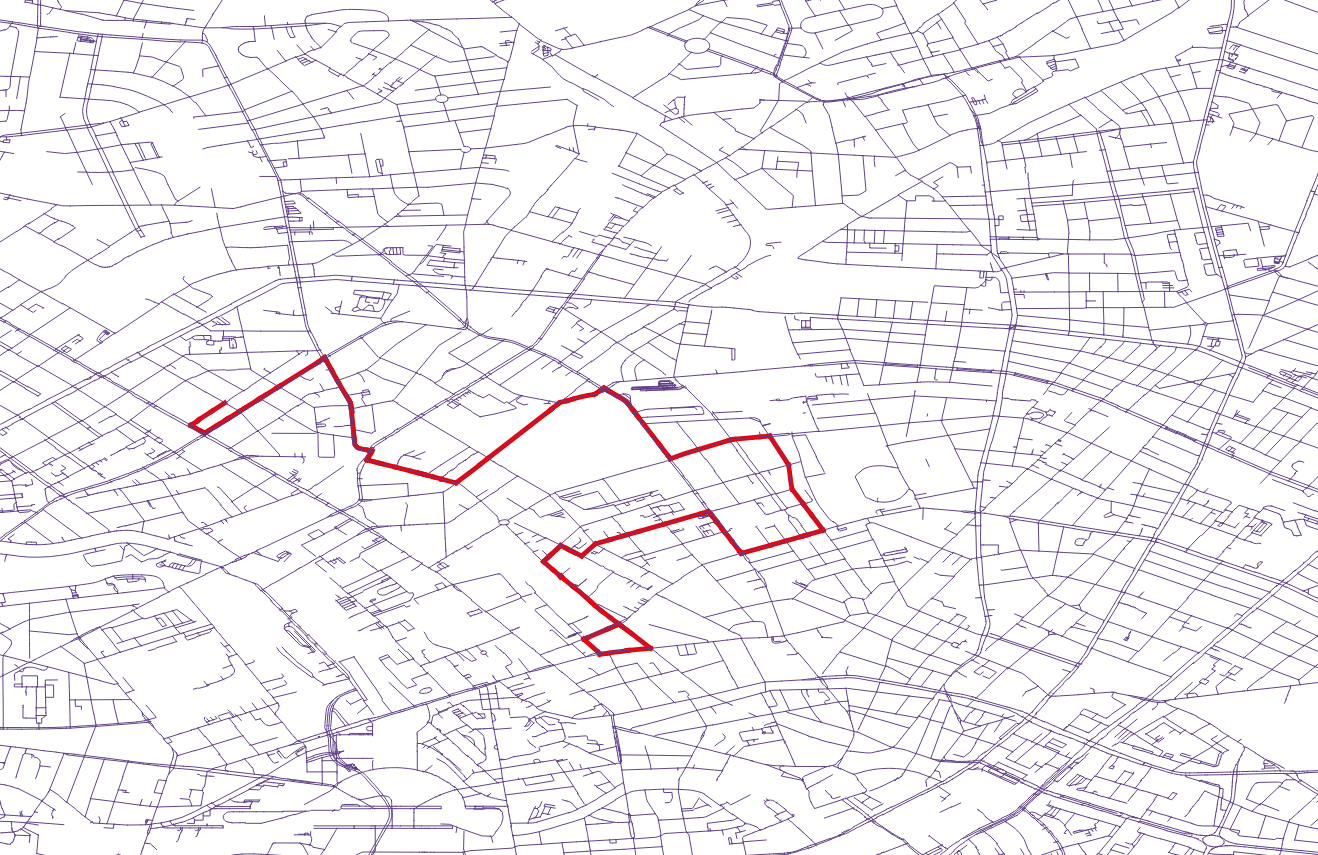
\includegraphics[scale=.25]{2.png}}
\hspace{5mm}
\subfloat[After Iteration 2]{ 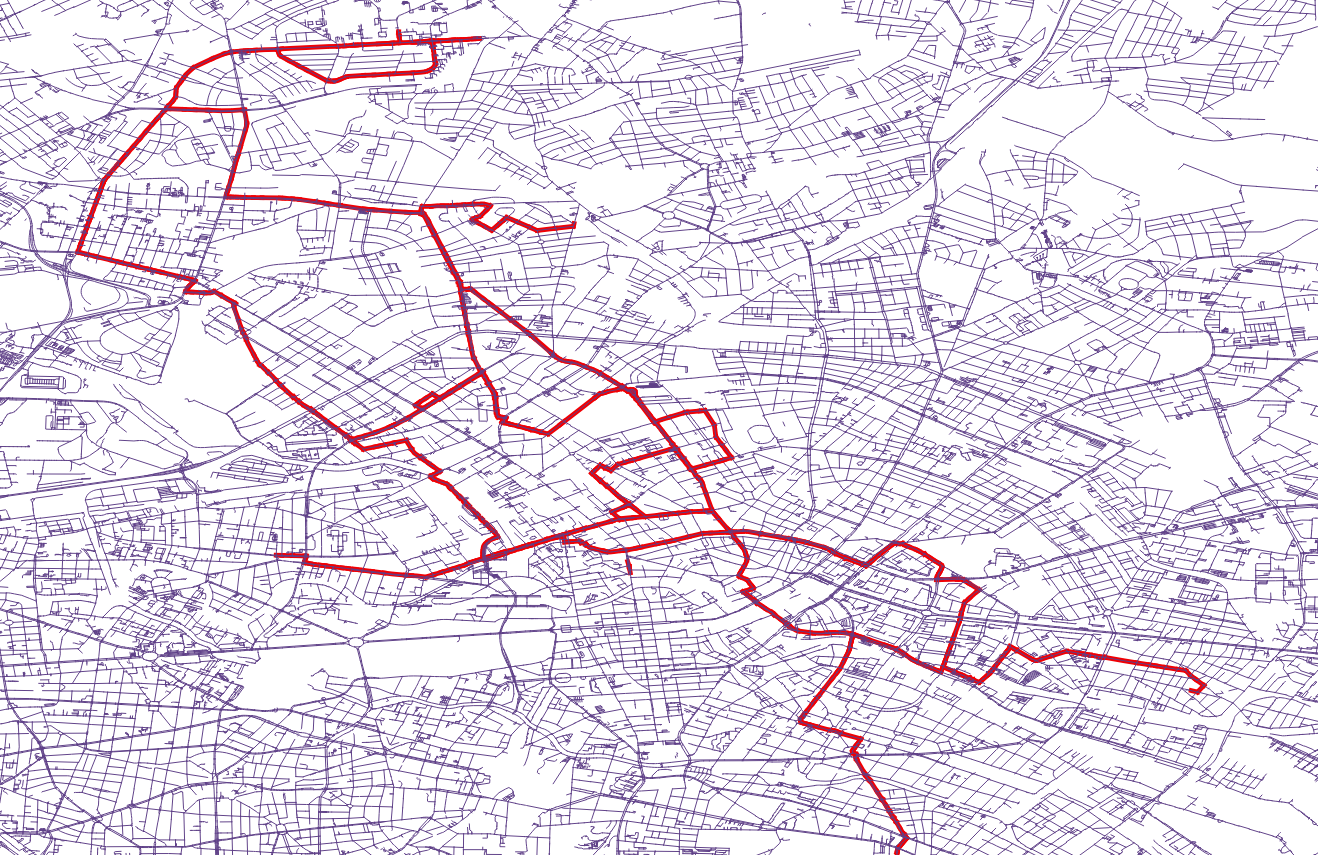
\includegraphics[scale=.25]{3.png}}
\subfloat[After Iteration 3]{ 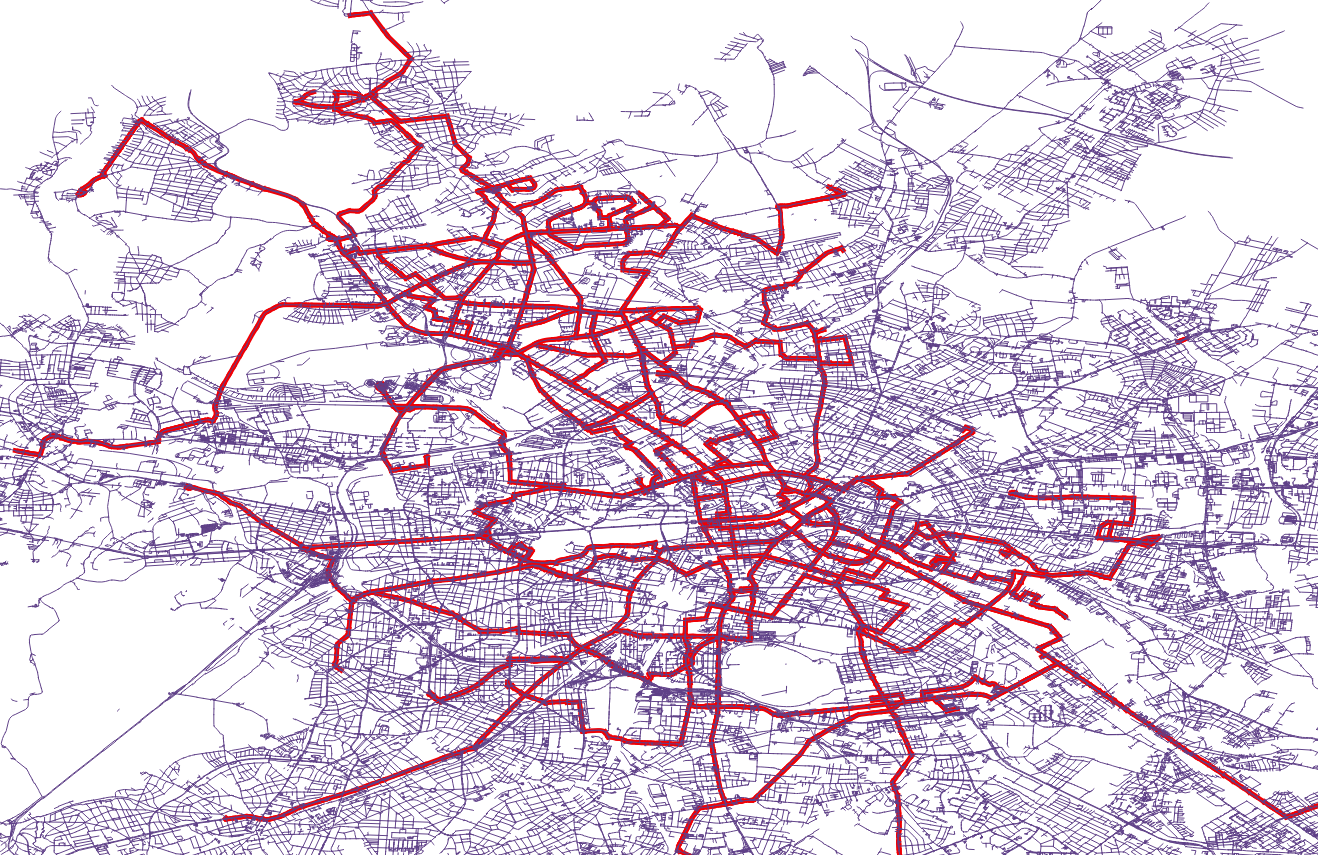
\includegraphics[scale=.25]{4.png}}
\hspace{5mm}
\subfloat[After Iteration 4]{ 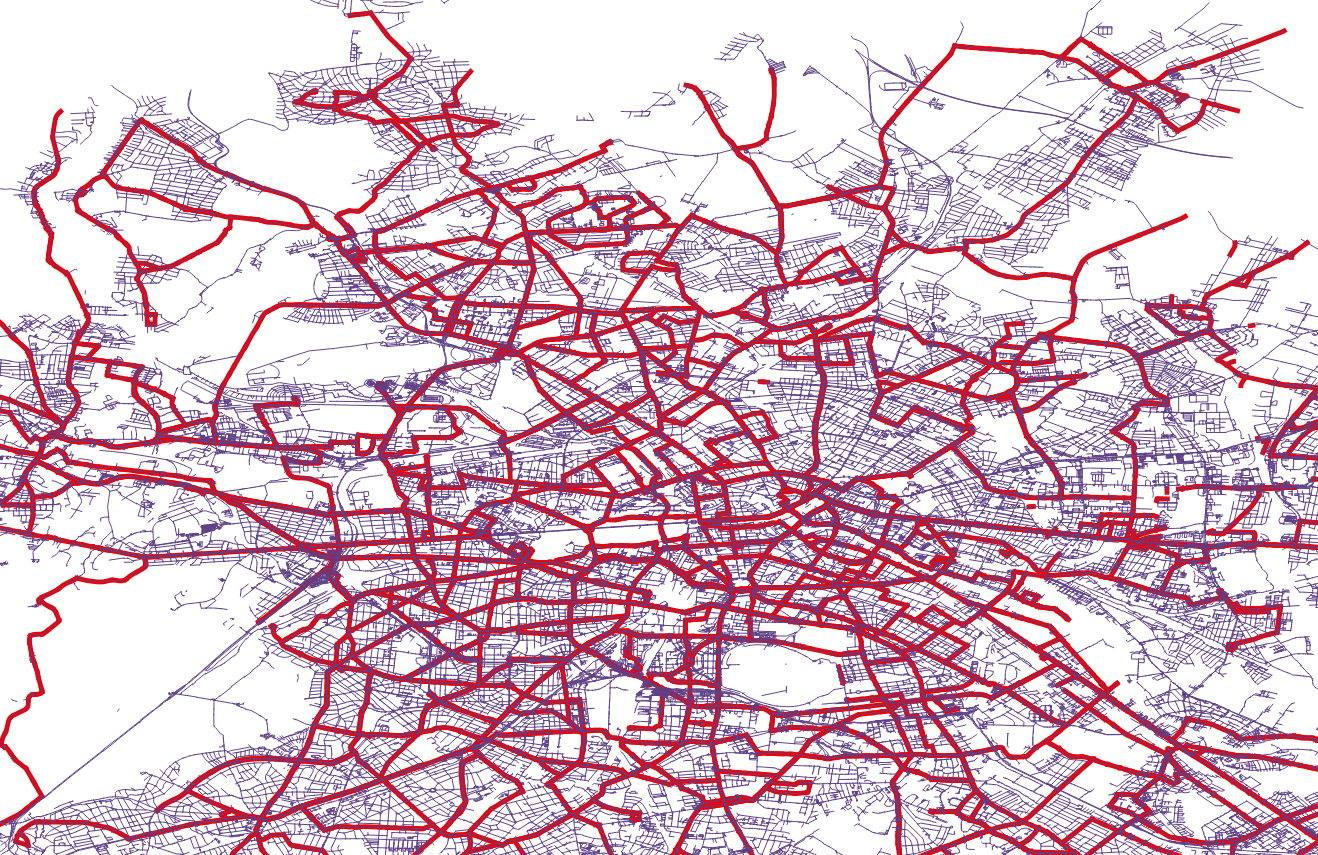
\includegraphics[scale=.25]{5.png}}
\subfloat[After Iteration 5]{ 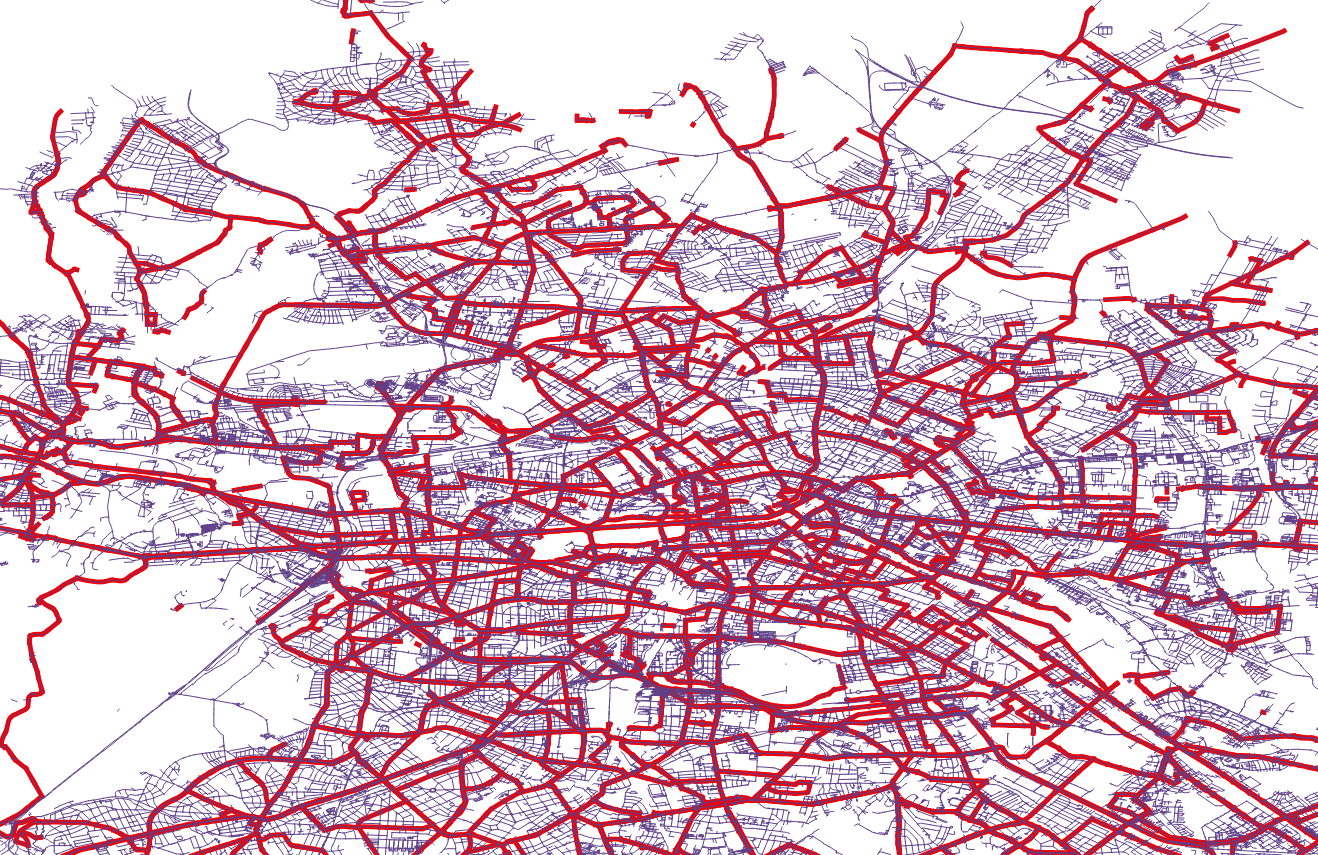
\includegraphics[scale=.25]{6.png}}
\caption{Results of a Breadth-first approach on map data of city of Berlin for one route calculation. The thin violet lines indicate streets in the map data and the red bold lines are the streets marked for update as identified in our algorithm during each iteration. The older map data represented date 30-Aug-2016 and the newer data is of date 31-Aug-2016.}
\end{figure}



%************************************************
\chapter{The Implementation}\label{ch:implementation} % $\mathbb{ZNR}$
In the last chapter, we presented our approach about the classification of map tile updates based on their relevance to the requested trip. We also discussed our Dynamic Map Update Protocol in detail. In continuation of our work, we present the implementation of our approach in this chapter. We discuss the tools which we used to build our evaluation setup, the specialized software packages and the database schema for the map database. We further discuss our process of utilizing the tools to create our evaluation setup using the map data in detail. 

\section{Why OpenStreetMap?}\label{whyosm}
In Chapter \ref{ch:introduction}, we discussed why high-definition maps are necessary for autonomous vehicles. These maps provide a very detailed virtual representation of the real world for a car to navigate safely. To the best of our knowledge for the current most common map formats for high-definition street maps, like OpenDrive \cite{opendrive} and the Navigation Data Standard with its Open Lane Model \cite{openlanemodel}, no public databases for testing and evaluation exist. These map formats, which can be used for highly automated driving, provide only small sample maps. They only demonstrate the capabilities of the specific map format. A map database with a long version history and a certain magnitude of applied changes however is necessary to properly test the capabilities of the Dynamic Map Update Protocol. To satisfy these requirements, we decided to use the available map material of the OpenStreetMap project \cite{haklay2008openstreetmap}. OpenStreetMap itself offers database dumps of its map material in intervals of up to one minute, one hour and one day between the newest database dump and its predecessor. The open source mapping project is community driven and has got a strong user base of volunteers. However, to resemble the update frequency of a high-definition street map into account, we selected the daily database dumps as the dataset to be tested with the Dynamic Map Update Protocol. By this decision, it is ensured that the map material of OpenStreetMap has a comparable amount of changes that can be expected for a high-definition street map in far less time (well below one day). Since the maintenance of map material is community driven, we selected the city of Berlin, Germany as the map material to be considered for the evaluation of our approach. The map material of Berlin is highly detailed compared to other areas of the world which are often mapped only very sparsely. This is due to the fact that the community of OpenStreetMap in Berlin is considerably active. This fact also ensures that the protocol is tested under realistic conditions for the scenario of highly automated driving. However it can be stated that the Dynamic Map Update Protocol can be applied to any form of navigational map, that includes a feature to weight the relevance of its content. The actual amount of data, which can be saved in the process of map updates will scale accordingly to its update frequency. As stated in Section \ref{geohashsizes}, the map is divided up into different layers regarding the type of streets. For the general evaluation of our approach we decided to group the street in two different layers. All the streets considered as highways by OpenStreetMap definition are grouped into one layer. All the other remaining streets form their own layer, for city streets. \\

\section{Tools}\label{tools}
We now discuss the variety of tool used in the evaluation of our approach. We also discuss their roles and key features which were used in the evaluation process. There are a variety of tools to process OpenStreetMap (OSM) files. Many of those tools are community maintained. There are some commercial tools as well. Only some of the community supported tools are regularly maintained. 

\subsection{PostgreSQL}\label{postgres}
As discussed in Section \ref{navasdb}, we required our map data to be availble in a database format. Being in a database format, allows us to design an approach which can query different objects and perform calculations to suit to our approach. PostgreSQL \cite{postgresql} is one of the many database softwares available today. It is an object-relational database management system (ORDBMS) which was initially released in the year 1996. It is widely deployed and supports many platforms, including various Linux distributions and Microsoft Windows. It is free and open-source software. However, it is maintained by a group of companies and individual developers known as PostgreSQL Global Development Group. It comes with a special license called PostgreSQL license, which allows free use. It is built to comply with standards such as ACID (Atomicity, Consistency, Isolation, Durability). This compliance allows it to extensible with the use of extensions which can be used in conjunction with the database to extend its functionality further. Such extensions expand the use of PostgresSQL database system in many application domains.
\\

PostgreSQL extensions allow it to be used for many different scenarios. Some of the data types supported by PostgreSQL are \begin{itemize}
\item Boolean
\item Character
\item Date/time (timestamp etc)
\item Numerics
\item HStore (extension to support key-value store)
\end{itemize} 
However, with the use of extensions more data types and functionality can be added to PostgreSQL. We used two such extensions in this thesis, PostGIS and pgRouting which are described later in this chapter. In this thesis, we used PostgreSQL version 9.3 running on a Ubuntu 14.04 LTS server.
\subsection{PostGIS}\label{postgis}
As we discussed previously (Section \ref{postgres}) that the functionality of PostgreSQL can be extended by the addition of compatible extensions. PostGIS \cite{holl2009postgis} is one of such extensions. PostGIS enables spatial database functionality in PostgreSQL. It allows storing of geographic objects in PostgreSQL. It also enables accessing those geographic objects using SQL queries. PostGIS also adds necessary functions, operators to support spatial database objects over the core functionality of a PostgreSQL database. geospatial objects could be queried and different analysis could be performed over a PostgreSQL database with a PostGIS extension enabled.  \\

PostGIS is compliant with "Types and Functions" of Open Geospatial Consortium ( \citet{lupp2008open} ). Due to such compliance, many other 3rd-party open source tools support working with PostGIS format. This also enables other extensions to be built-upon PostGIS to extend it further. pgRouting is one such example. It extends PostGIS functionality by providing different routing capabilities on geospatial data. The syntax to create PostGIS extension in a database is 
\begin{lstlisting} [frame=single]
~ $ psql mydatabase -c "CREATE EXTENSION postgis"
\end{lstlisting}


PostGIS is available as an extension of PostgreSQL. This enables PostgreSQL to provide the functionality as a backend spatial database server for GIS. Additionally, PostGIS is available under GPLv2 license. In this thesis, we used version {2.1} of PostGIS.
\subsection{pgRouting} \label{pgrouting}
One of the most used functions of navigation service is finding routes between two locations. To implement such functionality in our database, we looked for a suitable extension for the PostgreSQL database. The pgRouting project \cite{pgrouting} provides a library to extend functionality of a geospatial database to support routing and network analysis. It is an actively maintained open-source project. PostGIS enables us to query spatial data from a database. However, PostGIS alone is not sufficient for this thesis. The requirement to find the shortest path between two locations is crucial for this thesis. pgRouting has been developed over PostGIS extension to solve routing problems of real-life. Since, pgRouting is built over PostGIS extension, it is required to create 'postgis' extension in the database before creating 'pgrouting' extension. 
\begin{lstlisting} [frame=single]
~ $ psql mydatabase -c "CREATE EXTENSION postgis"
~ $ psql mydatabase -c "CREATE EXTENSION pgrouting"
\end{lstlisting}

pgRouting offers advantages over other traditional routing approaches \begin{enumerate}
\item it is easy to modify objects, 
\item supports a different variety of clients to perform operations, 
\item updated results could be fetched by running query again and 
\item different formulas can be applied to calculate the route cost.
\end{enumerate}

Similar to PostGIS, pgRouting is available under GPL2 license. pgRouting is being actively maintained. With new major releases, new functions to extend the functionality are added. Sometimes due to change in function signature, the code could break. Hence, the version of pgRouting extension is important when replicating this work. For this thesis, pgRouting extension compatible with PostGIS is used to extend the functionality of our spatial PostgreSQL database server. In this thesis, we have used pgRouting extension version 2.1. 


\subsubsection{pgRouting Features}
In addition, to provide a routable spatial database, pgRouting \cite{pgrouting} supports a wide variety of shortest path algorithms to address the problem of finding different paths between two locations on a map. Many popular shortest path algorithms such as Dijkstra and A-star are supported by pgRouting. It provides different functions to make use of the algorithms.We used Dijkstra shortest path function in our work during this thesis. The syntax for using the Dijkstra shortest path in pgRouting is listed below. 
\begin{lstlisting} [frame=single]
pgr_dijkstra(text edges_sql, bigint start_vid, bigint end_vid,
                   boolean directed:=true);
   RETURNS SET OF (seq, path_seq, node, edge, cost, agg_cost) or EMPTY SET
\end{lstlisting}
The function listed above can be used for calculating a shortest path using Dijkstra's algorithm from the vertex referred by start{\_}vid to the vertex end{\_}vid  
\begin{itemize}
\item	on a directed graph when directed flag is missing or is set to true.
\item	on an undirected graph when directed flag is set to false.
\end{itemize}

\subsection{Osmosis} \label{osmosis}
In Section \ref{postgres}, we discussed our geospatial database server configuration using PostGIS (Section \ref{postgis}) and pgRouting (Section \ref{pgrouting}) extensions. Now we required to process map data and add it to our geospatial database. For the scope of this thesis, we used Osmosis to process OSM dump files available in a highly compressed 'Protocolbuffer Binary Format' pbf format \cite{osmpbf}. PBF format provides an alternative format for storing OSM data in XML file format. The format provides significant reduction in map data files for a large region. In addition to reducing file size, the PBF format allows faster read and write operations as well. It is fully compatible with OSM's XML format and the open format allows many tools to support it. \textit{Osmosis} \cite{osmosis} is a Java based utility to work with OpenStreetMap (OSM) data. It offers a command line interface to perform various tasks such as extracting specific elements from map data, conversion between different map file formats etc.. While choosing a tool to process highly compressed 'Protocolbuffer Binary Format' \textit{pbf} files into a more readable \textit{osm} format, we came across options like \textit{pbftoosm} \cite{pbftoosm} and \textit{Osmosis}. Although \textit{pbftoosm} is a faster alternative \cite{pbftoosm} to \textit{Osmosis} to decompress highly compressed pbf files into \textit{osm} files, it is not actively maintained. We decided to choose \textit{Osmosis} because of its large community and active support. It also offers additional functionality with pluggable modules. \\

Our requirements from the tool were
\begin{enumerate}
\item Reading and writing in different formats of OpenSteetMap data, and
\item Extracting map data inside a polygon or bounding box
\end{enumerate}
Osmosis covered all our requirements for this thesis. Additional features provided by Osmosis include \begin{enumerate}
\item Reading and writing from various sources, including database, files etc.
\item Filtering OpenStreetMap data
\item Generating planet dumps from databases
\item Producing change sets between two OpenStreetMap files
\item Applying change sets 
\end{enumerate} 
These are some of the features provided by Osmosis. For larger applications, it can also be used as a linked library for custom applications.\\ 

A public repository of Osmosis is available at GitHub \cite{osmosis}. Using Osmosis, we were able to decompress .osm.pbf (Protocol Buffer Format) files to .osm (OSM XML) files. The syntax for such operation is 
\begin{lstlisting}[frame = single]
~ $ osmosis --read-pbf berlin.osm.pbf --write-xml berlin.osm
\end{lstlisting}

We also used osmosis to extract data inside a polygon to obtain OSM data for a particular city. Syntax for that is
\begin{lstlisting}[frame=single]
~ $ osmosis --read-pbf country.osm.pbf --bounding-polygon \
    file="city.poly" --write-xml city.osm
\end{lstlisting}

\subsection{osm2pgrouting} \label{osm2pgrout}
In previous Section \ref{postgres}, \ref{postgis} \& \ref{pgrouting}, we discussed how geospatial databases are necessary to provide map data as database to be able to process. We also discussed how we could extend the functionality of the PostgreSQL database server as a geospatial database backed by using extensions. We discussed PostGIS and pgRouting extensions and their use in the setup for this thesis. Since map data from OpenStreetMap is not readily available in a usable database format, we need to process it. We required a tool to process data from \textit{osm} files and put into the geospatial database we created using PostgreSQL. osm2pgrouting does just that. osm2pgrouting is an open-source project to import OpenStreetMap (OSM) data files into a PostgreSQL database which can be processed by PGRouting further on. 
\\

osm2pgrouting is maintained by the same community that is behind pgRouting. It is written in C++. It has a command-line interface which allows you to pass different configurations via options. Complete syntax for using osm2pgrouting can referred at its github page \cite{osm2pgrouting}. In earlier chapter, we described an XML like \textit{osm} file format. osm2pgrouting parses OSM data and processes before storing it into the database. The database parameters are passed via command-line arguments. If '--addnodes' option is enabled, osm2pgrouting also stores OSM node data in the database. Various configurations for routing related information is passed through a configuration file. \textit{osm} file data is not limited to just road network for cars. It also has information about walking paths and bicycle paths. We needed to filter out such paths where a car cannot be used to be able to simulate real-life navigation scenarios. Hence, in this thesis we used the map configuration for cars which is available within the osm2pgrouting package. \\

\subsubsection{Modifications to osm2pgrouting} \label{modifications}
In Section \ref{osmosis} \& \ref{osm2pgrout}, we described how we process OSM data available through map dumps in the pbf file format into routing enabled geospatial database with the use of osm2pgrouting. While osm2pgrouting works quite well for processing OSM data into a pgRouting compatible format in a spatial database, it is not designed to store any version/history related information. We described in the earlier part of this thesis about how maps change over time. New roads are mapped and added, non-existing roads are deleted. With the goal of tracing changes in a map for this thesis, it was crucial to have a version and time-stamp information extracted and stored in geospatial database. With no other tool available to fulfill these requirements, we decided to extend existing the existing functionality provided by osm2pgrouting to include the version and time-stamp information in spatial database. \\

These changes required to parse and process version \& time-stamp information. They also required modifications in the database schema to include these additional information. We had to add extra columns in 'nodes' and 'ways' table. The additional columns are 'version' and 'time-stamp'. We managed to incorporate these additional functions in osm2pgrouting. The source code and building instructions for the modified tool can be accessed at \cite{sharma2016}. 
\section{Database Schema}\label{dbschema}
Through the use of pgRouting and PostGIS extensions in PostgreSQL, we created a spatial database to support routing queries over the map data. We used osm2pgrouting to read the map data present in respective .osm files and to process and write it into the database. Upon successful completion, the map data is loaded in the spatial database which we created earlier. The schema of the whole database is shown in Figure \ref{fg:db}. After processing the map data, only a selected portion of the information provided in the osm file is stored in these 9 tables. The tables \textit{osm{\_}relations} and \textit{spatial{\_}ref{\_}sys} are not relevant to this thesis work. We now explain the use of the different tables and the structural modifications which had to be applied to some of them in the progress of the thesis.

\begin{figure}
\centering
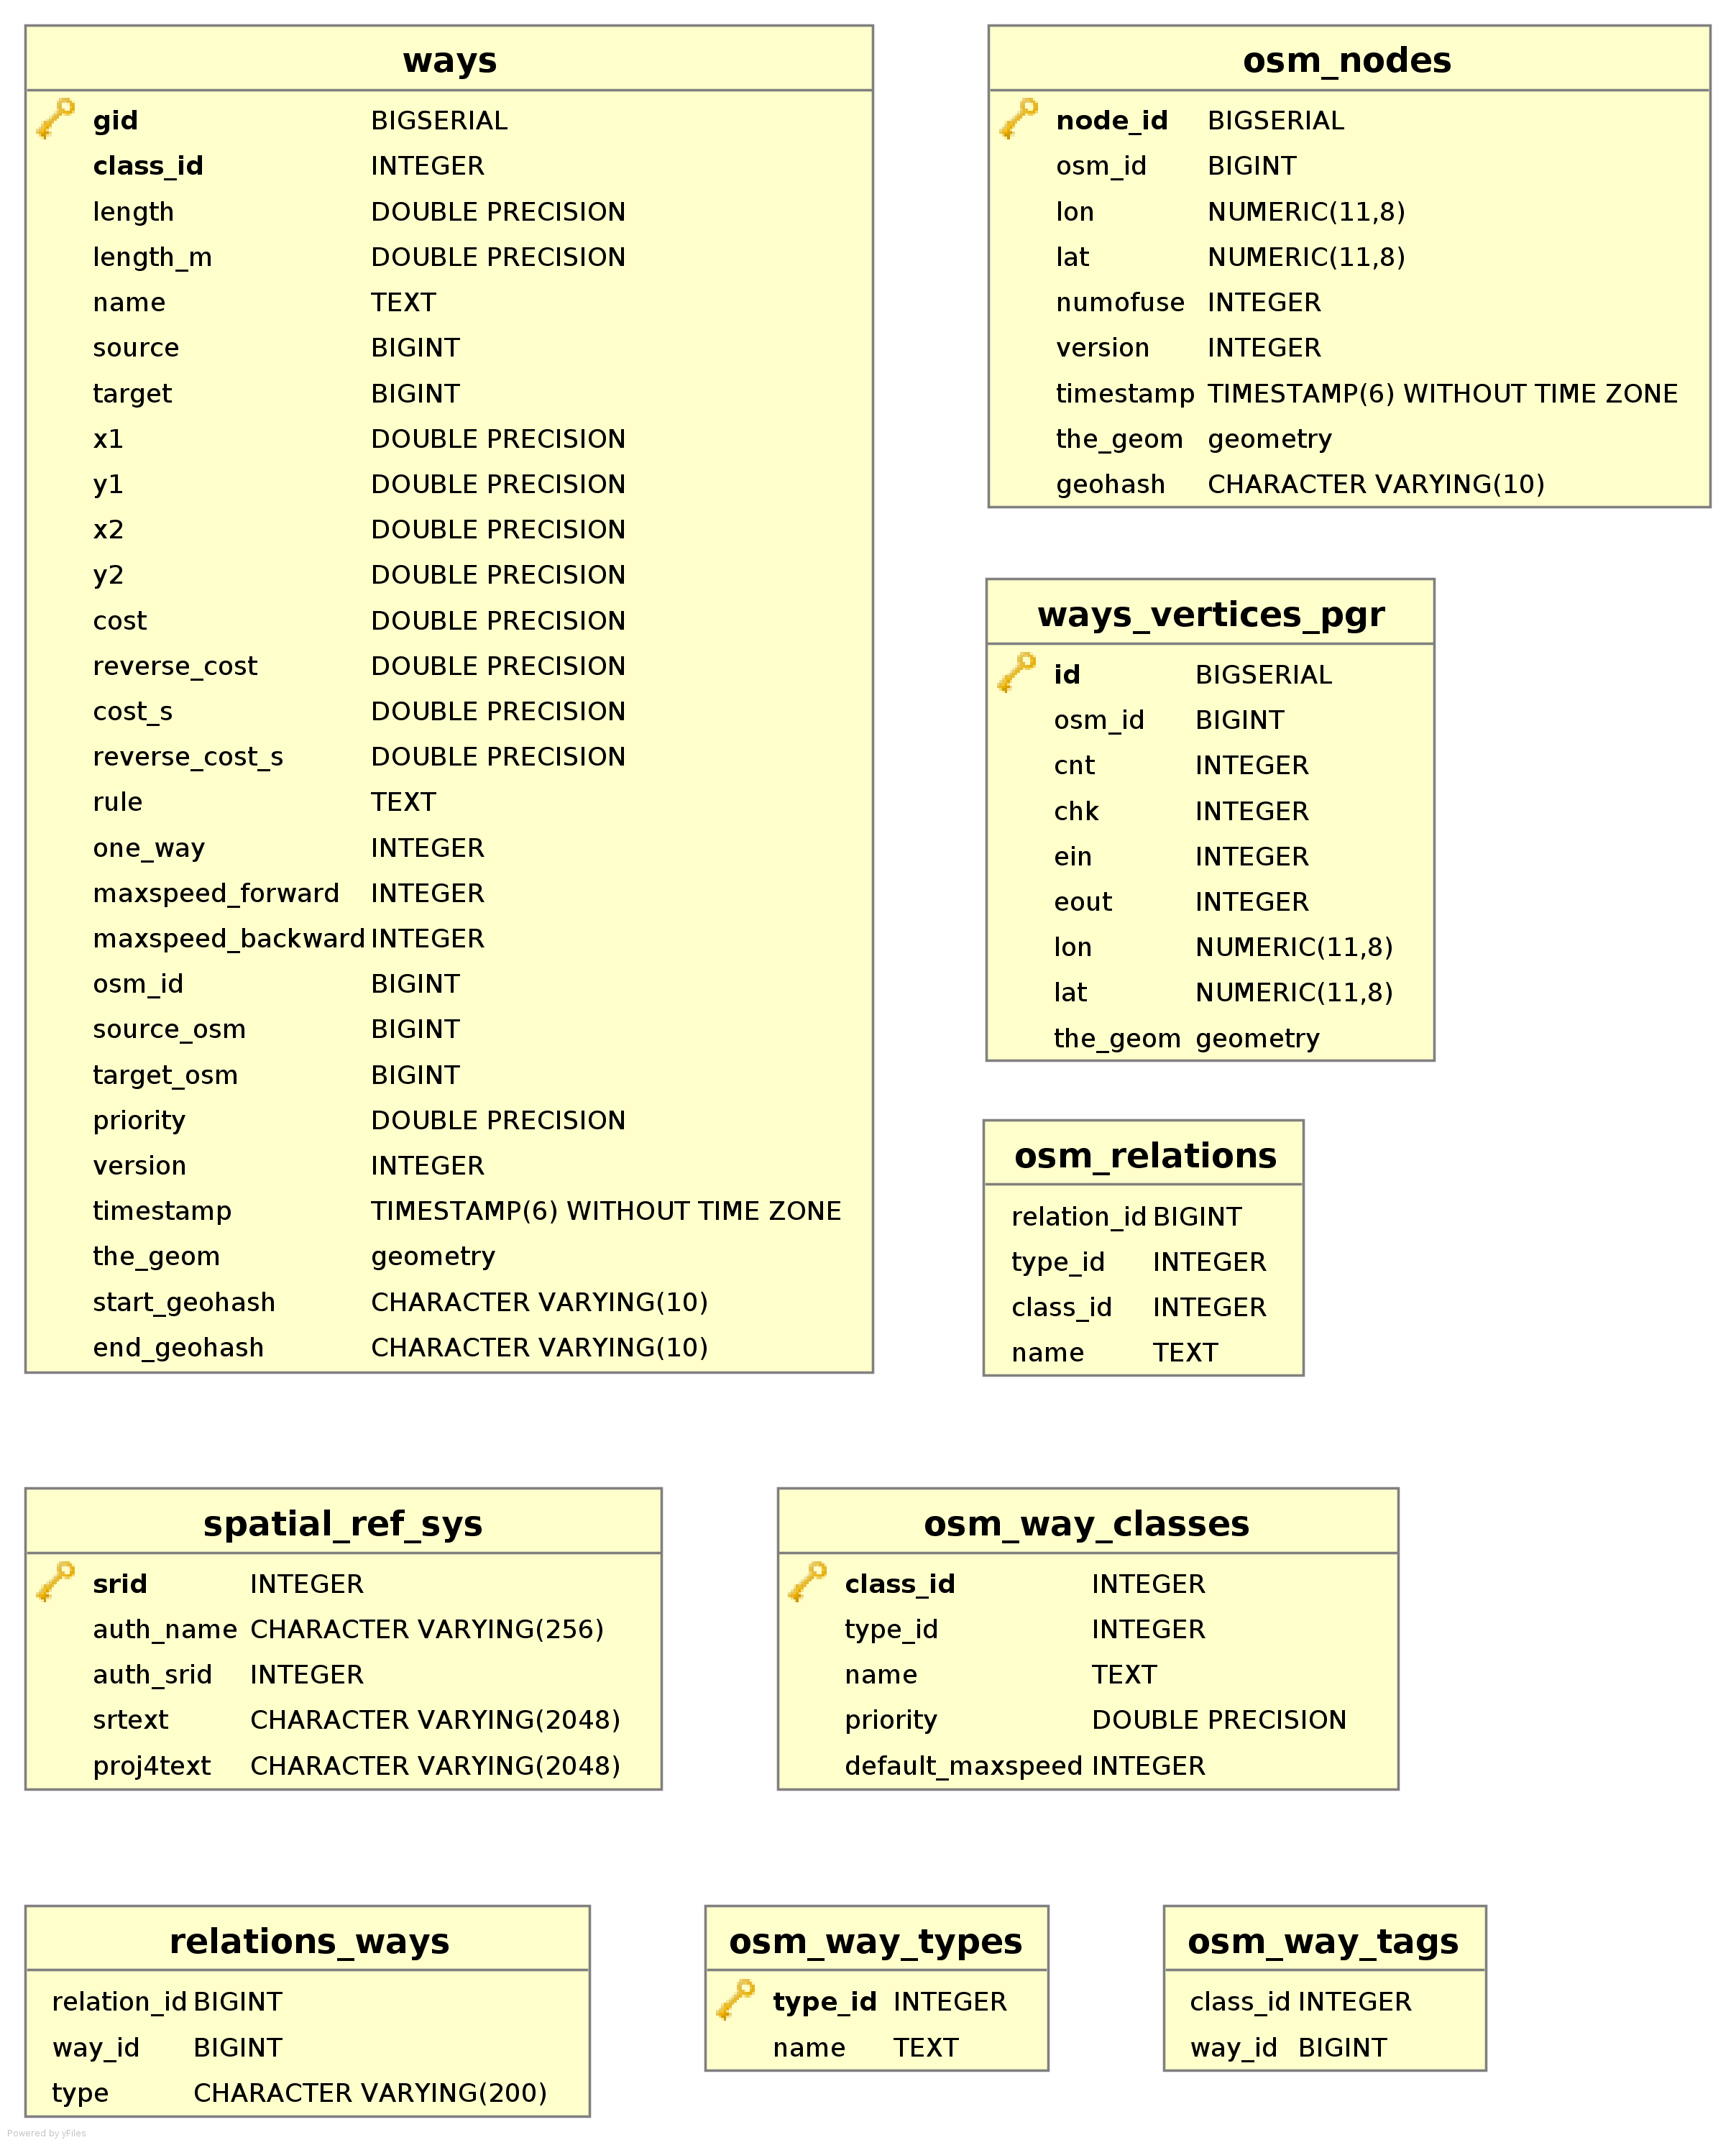
\includegraphics[scale=.2]{pgrouting.png}
\caption{The complete database schema of pgRouting database.}
\label{fg:db}
\end{figure}



\subsection{Table: osm{\_}nodes}
In Section \ref{osmosis} we covered how we used \textit{Osmosis} tool to decompress \textit{pbf} files to generate XML based \textit{osm} files for futher processing. With the help of a modified version of \textit{osm2pgrouting} tool, we processed the map data stored in \textit{osm} file and import it in our spatial database running over PostgreSQL database (see Section \ref{postgres}). The \textit{osm2pgrouting} tool processes the map information stored in the \textit{osm} file and stores it into a database format to support routing functions provided by pgRouting. After this processing, in the database a table named osm{\_}nodes is filled with information about all nodes read from the .osm file. The structure of the table is explained in Figure \ref{fg:osmnodes}. Due to our additional requirements ( see Section \ref{modifications} ), we introduced the new columns 'version', 'timestamp' and 'geohash' additionally in this table. The columns 'version' and 'timestamp' contain information about the version of the nodes in the table. And the 'geohash' column contains each node's corresponding geohash value. 
\begin{figure}
\centering
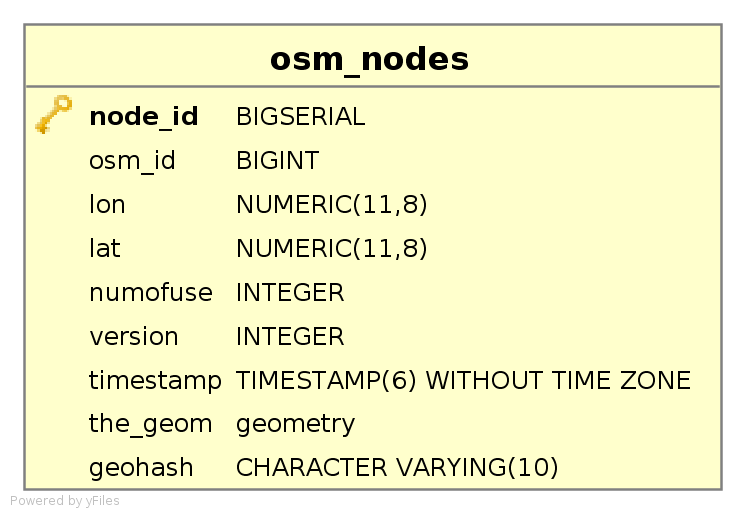
\includegraphics[scale=.3]{osmnodes.png}
\caption{Schema of table osm{\_}nodes.}
\label{fg:osmnodes}
\end{figure}

\subsection{Table: ways}
OSM ways are one of the data primitives of OpenStreetMap data as described in Section \ref{osmxmlff}. The ways contain information about the paths on the map. All information regarding the ways is stored in the database table with the same name. The schema of the table \textit{ways} is shown in Figure \ref{fg:ways}. Each way is divided up into multiple segments which form the complete path. The efficient route calculation of segments is required to enable the graph analysis functions of pgRouting. This allows the efficient route calculation. The column 'osm{\_}id' refers to the unique identifier of each path, however a newly generate 'gid' is used as the primary key in this table. The column 'class{\_}id' refers to the class of the road, such as highway, residential etc. which were explained in Section \ref{osmxmlff}. Additionally, columns 'start{\_}geohash' and 'end{\_}geohash' have been added to speed up queries by \textit{geotagging}. The column 'start{\_}geohash' stores the geohash value (Section \ref{geohash}) of the starting point of the path and the column 'end{\_}geohash' stores the geohash value of the terminating point of the path segment. These geohash values are calculated based on the road type identified by the column 'class{\_}id'. Similarly to the table for nodes, additional columns for 'version' and 'timestamp' have been added for the requirements explained in Section \ref{modifications}. Additional information derived by calculations such as the distance between the start and the end point of a path and the cost of traveling on it, derived from the maximum speed allowed on the road is added in the table as well as the new columns. Restrictions such as one-way streets which affects routing calculations are also added in this table. It is the largest and most important table in the database, since it is read most frequently compared to all other tables to process the routing queries. Thus, to increase the performance of the overall procedure some of the information contained in it is duplicated in other smaller sized tables such as \textit{osm{\_}way{\_}classes}.   
\begin{figure}
\centering
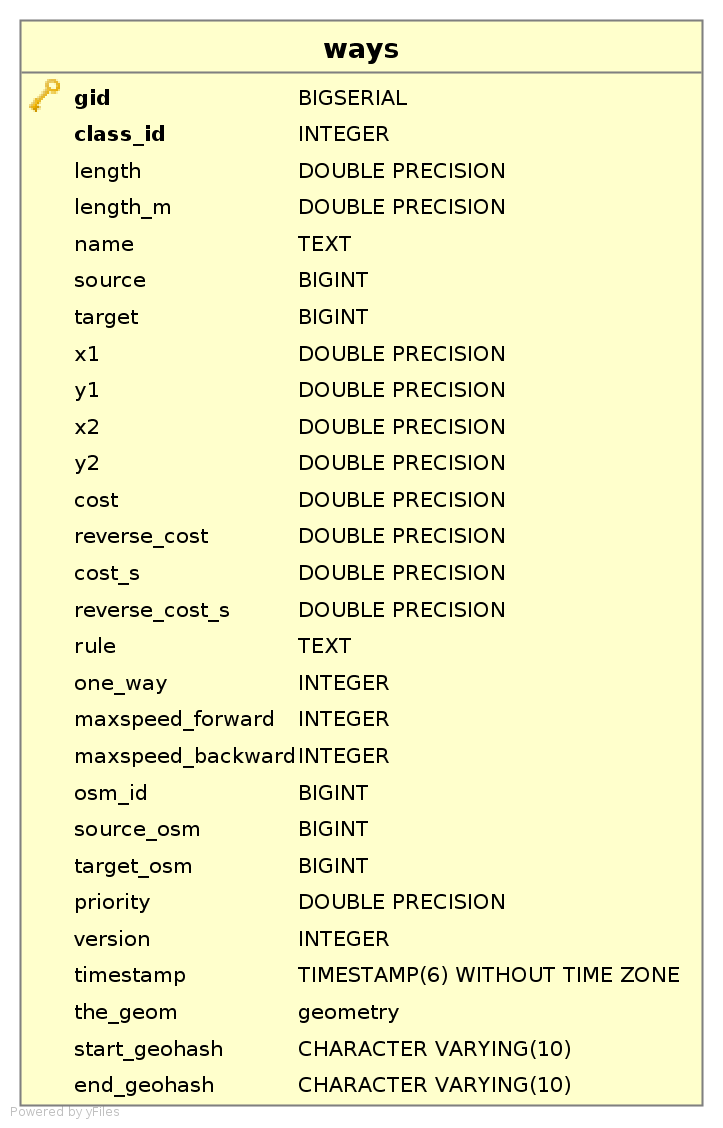
\includegraphics[scale=.35]{ways.png}
\caption{Schema of table ways.}
\label{fg:ways}
\end{figure}

\subsection{Table: ways{\_}vertices{\_}pgr}
The table \textit{ways{\_}vertices{\_}pgr} is filled after processing data from each way present in the osm input file. The schema of the table is shown in Figure \ref{fg:waysverticespgr}. After filling table \textit{ways}, further processing is applied to load only vertices in the table \textit{ways{\_}vertices{\_}pgr}. One entry per osm{\_}id is loaded into the table \textit{ways{\_}vertices{\_}pgr} which represents each way object. Multiple entries per osm{\_}id are loaded into table \textit{ways} due to the splitting of ways into smaller segments for turn-by-turn navigation queries. Often, the intersection between two different ways is marked and identified as a vertex in this table. The vertices in this table represent different vertices in a connected graph which is the representation of the road network of an area. The vertices as the column 'id' values from this table are used for querying the shortest path between two locations. The corresponding location of the vertex for each entry is stored in the columns 'lon' and 'lat' of this table.
\begin{figure}
\centering
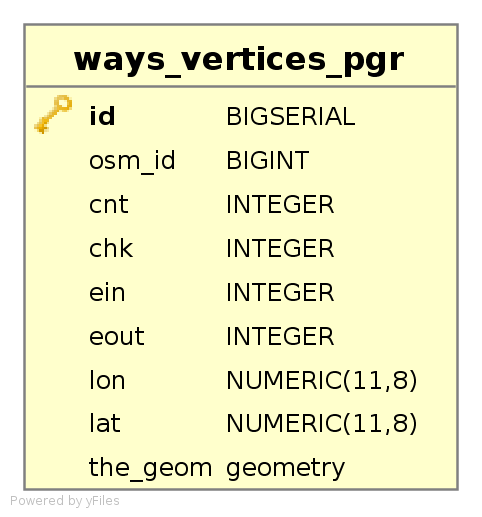
\includegraphics[scale=.31]{waysverticespgr.png}
\caption{Schema of table ways{\_}vertices{\_}pgr.}
\label{fg:waysverticespgr}
\end{figure}

%\subsection{Table: osm{\_}relations}

%\begin{figure}
%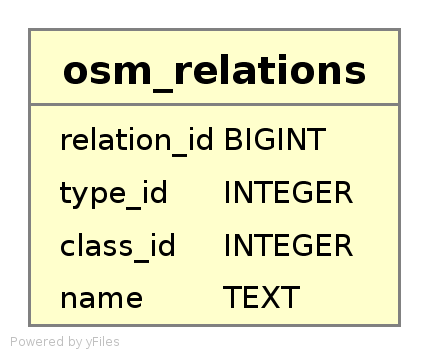
\includegraphics[scale=.26]{osmrelations.png}
%\caption{Schema of table osm{\_}relations}
%\label{fg:osmrelations}
%\end{figure}


\subsection{Table: osm{\_}way{\_}classes}
Figure \ref{fg:osmwayclasses} shows the schema of the table osm{\_}way{\_}classes. The information about different road classes and the routing priorities of those classes of roads is stored in this table. As explained earlier in Section \ref{tag}, different streets in OpenStreetMap are identified by their class definition, such as a highway or a city street. This information is important to understand the type of road and relatively the maximum allowed vehicle speed on that street. The class of the road is identified while reading the tag (Section \ref{tag}) associated with a way in an osm input file. The shortest path routing functions provided by pgRouting extension (see Section \ref{pgrouting}) use priority information provided in this table to find the optimum path between two locations on the map. The priority information associated with a 'class' of street is useful in calculating the cost of each edge in a map which is represented as a graph. The information about different ways/road types, their default maximum speed, their assigned \textit{class{\_}id} values, and the priority (\textit{lower number indicates higher priority}) is stored in this table. The priority values are used by routing algorithms to prefer certain roads based on their value. By default, the priority column is loaded with values in such a way that it prefers a highway road over a city street resulting a routing result preferably using a route using a highway between two locations, if exists. \\

The column 'class{\_}id' stores a predefined value for different classes of roads according to the OSM specification (see Section \ref{tag}) are generated starting from the value of 101. These values are referenced in other tables such as \textit{ways} for determining the cost of each road segment in routing. Each class of a road segment has an associated value of legal limit of the speed. As explained earlier, a priority value is also associated with each class of roads in this table. However, the priority value is a modifiable component of pgRouting. Any modifications to the priority value can result in different routing results. Any modifications to this table, such as default{\_}maxspeed and priority can directly affect the routing results returned by pgRouting functions (Section \ref{pgrouting}) of the spatial database. It is possible to modify this table to suit some different routing requirements, however for our thesis, we did not do any modifications to this table.  
\begin{figure}
\centering
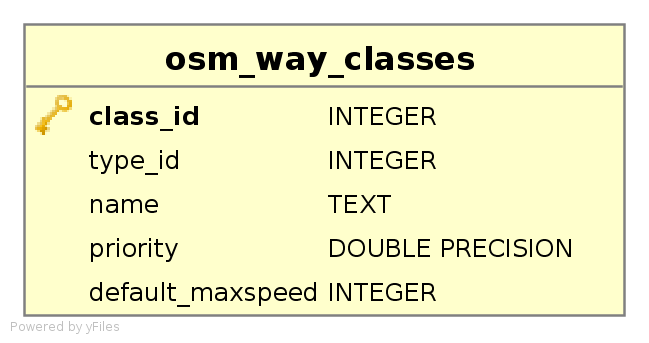
\includegraphics[scale=.31]{osmwayclasses.png}
\caption{Schema of table osm{\_}way{\_}classes.}
\label{fg:osmwayclasses}
\end{figure}


%\subsection{Table: spatial{\_}ref{\_}sys}

%\begin{figure}
%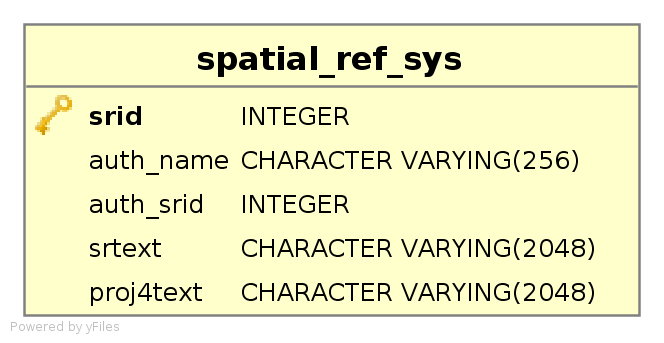
\includegraphics[scale=.31]{spatialrefsys.png}
%\caption{Schema of table spatial{\_}ref{\_}sys}
%\label{fg:spatialrefsys}
%\end{figure}


\subsection{View: wayshashed}
The protocol (Section \ref{protocol}) in our approach depends on the use of the segmentation of the used map into specific grids and their versioning to identify whether a particular grid has changed in the newer version of the map or not. There is no implicit grid based geotagging mechanism provided by pgRouting (Section \ref{pgrouting}). In our post-processing of the database (Section \ref{postprocessing}), we have used a Geohash (Section \ref{geohash}) based scheme to place a grid indexing structure on the existing map data. However, for our protocol, we required a way to identify different versions of a grid. To solve the problem of versioning of grids, we have used a view for storing grid related information to identify different versions of the grid. It is implicitly assumed that the map server will always have the most recent version of the map and the grids in it. The schema of the view \textit{wayshashed} is shown in Figure \ref{fg:wayshashed}. The column 'geohash' refers to each grid identified by its geohash. The most recent timestamp value in a grid is stored in the corresponding column 'recent' of the view \textit{wayshashed}. The count of all the objects in a particular grid is stored in column 'count' while the column 'version' stores the sum of version of each individual element present in the grid. Comparison based on the values of the columns 'recent', 'version' and 'count' is used to detect whether the elements of a particular grid have changed or not. Any such change in a grid of two different versions of a map will be detected by comparing these values from the view \textit{wayshashed}.
\begin{figure}
\centering
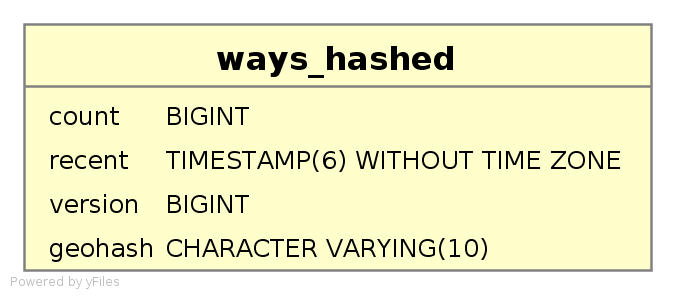
\includegraphics[scale=.3]{wayshashed.png}
\caption{Schema of view wayshashed}
\label{fg:wayshashed}
\end{figure}



\section{Process} \label{process}
In the previous section, we described all the necessary software tools we used during this thesis work. We discussed our database server and necessary extension for it to make a geospatial database server. We also covered tools such as Osmosis to decompress pbf files into regular \textit{osm} files and osm2pgrouting which processes and stores OSM data into our database server. We also discussed the modifications we had to do in osm2pgrouting specifically for this thesis work. In this section, we are going to discuss the process of preparing database and other necessary setup for evaluation. The overall pre-processing process of the osm map data as shown in Figure \ref{fg:process} is comprised of several steps which we are going to cover in detail in the following sections. 

\begin{figure}
\centering
\includegraphics[scale=.6]{process.png}
\caption{The Process for our implementation, includes processing of map data files into the database and evaluation procedure.}
\label{fg:process}
\end{figure}

\subsection{Getting OSM Data}\label{data}
To work on different versions of map data, we required map data from different days. Therefore multiple ways to download OSM datasets exist. Full OSM dataset for example are available at the OSM website \cite{planetosm}. One of the options available at this page is to download the history file for whole planet earth. This history file contains all the changes that have been made into OpenStreetMap since the beginning of the project. However, this file did not satisfy our requirements as we could not generate different \textit{osm} files for specific dates out of it. After researching for alternative possibilities, we considered the data extracts of OSM which are provided by a company Geofabrik GmbH \cite{geofabrik}. \\

Geofabrik \cite{geofabrik} maintains downloaded data extracts of OpenStreetMap for different regions of the world. They are categorized hierarchically from continents to states inside a country. Most of the countries worldwide therefore are available as distinct OSM extracts on their website. Through using their provided data, we collected extracts of the year 2014 and 2015 as well as of every month of 2016. Geofabrik's website also provides daily dumps of the last 2 days on their website. We decided to consider different regions worldwide to be analyzed in this thesis. Over a period of 2 months and a few days, we downloaded daily dumps of these regions. These daily dumps then were used as input for the further pre-processing, are available with filenames in format <region>-<date(YYMMDD)>.osm.pbf.

\subsection{Decompressing pbf->osm}
The data extracts provided by Geofabrik are provided in the Protocolbuffer Binary Format (PBF) \cite{osmpbf} as described earlier in Section \ref{data}. The PBF format is a highly compressed alternative format to OSM's XML format. The format also allows much faster read and write operations when dealing with map data in a file format compared to the OSM's XML format. However it is not yet supported by the pgRouting toolkit which we require for the further steps of processing. For compatibility with the pgRouting tool, we first need to convert the \textit{pbf} files into the \textit{osm} file format. Therefore we used Osmosis, which is able to convert the data, as described in Section \ref{osmosis}. After selecting which region and dates to consider for evaluation, we wrote a simple bash script to invoke Osmosis for this conversion. The time required by Osmosis for conversion is related to the file size of the map data to be processed. For example, a 278 MB PBF took 167 seconds to be converted into an OSM file on a laptop powered by Intel i5 processor with 8GB of RAM. The resulting osm file had the size of 6963 MB (25x larger).
\subsection{Importing Data into the Database}
After converting the \textit{pbf} file into the \textit{osm} format, we use our modified version of the \textit{osm2pgrouting} tool to import the OSM map data into our database. As explained in the osm2pgrouting manuals \cite{osm2pgrouting}, we use following parameters 
\begin{lstlisting} [frame=single]
~ $ osm2pgrouting -f ./<mapfile>.osm -c ../mapconfig_for_cars.xml \
    --addnodes -d <database name> -h <server ip address> \
    -u <postgres username> -W <password>
\end{lstlisting}

The tool is designed to read the \textit{osm} files and parse it to store different OSM objects in a database structure as explained in Section \ref{osmxmlff}. Afterwards, it performs the necessary actions to make the map data compatible with pgRouting by breaking roads in vertexes of a graph. This process is memory intensive. We recommend to use a machine with almost ~1.5x times available memory than the size of the map in \textit{osm} format to be processed. Once the process is successful, we can begin post-processing database for additional data that we require. 
\subsection{Post-processing of the Database} \label{postprocessing}
To optimize the query process for identification of relevant map updates, we required additional information from the geospatial database about map objects. This information includes grid information, a grid versioning system, changes between different versions of a grid and an index table to link map objects to a grid. Such information can also be calculated on the fly, however having them stored in the database saves computing time and additional queries to the map database. Such information has to be prepared once and only updated if there are changes applied to the database. This includes the generation of Geohash based grids and the versioning for those grids. As discussed in Section \ref{geohash} we require the functionality of Geohashes to divide our map up into useful grids, since there is no inherent grid system built into OpenStreetMap. OpenStreetMap classifies its street network into different categories of streets as described in Section \ref{osmattributes}. While processing the map data, osm2pgrouting extracts this information and stores it in the table 'osm{\_}way{\_}classes' as described in Section \ref{dbschema}. We use this information in the Dynamic Map Update Protocol to further decrease the amount of data to be transmitted, since only the specific layers of roads which are used by the client than have to be provided by the server. For the simplification of the implementation, we decided to distinguish only between two different classes, namely the highway and the city streets. The concept, however can be extended to further layers of different road types to further decrease the amount of data that needs to be provided. 
\\

By referring to the information provided in the table 'osm{\_}way{\_}classes' (Figure \ref{fg:osmwayclasses}), we can infer that if the 'class{\_}id' is between 101 and 111, it is a highway. If any other ID is given the street will be categorized into the 'city-street'-layer. In Section \ref{geohashsizes}, we discussed how the precision affects the grid size represented by a GeoHash. We use Geohashes with a precision of 4 digits for representing larger grids with highways. And we use precision level 5 for representing smaller grids for the remaining classes of roads. As we explained in Section \ref{geohash} that geohashes are calculated based on latitude and longitude values of a point. With respect to ways, we calculate two geohashes per way. These are called 'start{\_}geohash' and 'end{\_}geohash'. As the name suggests, they are geohashes of start and end position of a way.
\\

Only the OSM objects are versioned in OpenStreetMap. Thus, we also needed a mechanism to detect a change in a grid between two different dates. To achieve this, we created a database view based on the information about each individual grid in the map in the database. We use this information to detect whether a change has been there or not in a grid. We use the combination of the most recent time-stamp of any way in a grid, a sum of version numbers of ways inside grid as a composite version indicator. If there are changes in a particular grid, it is very likely that either of these indicators will change.
\\

We aimed to compute most of the data required to compute update on the fly, it would certainly slow us down if there are multiple queries to the database, both at client and server's end. It would certainly add an unnecessary overhead while computing the updates required. Similarly, geohashes can be computed while processing a navigation request. However, that would require to read all the latitude and longitude information of the ways. To keep the overhead to a minimum, we decided to pre-calculate this information and store it in our geospatial database. We saw more than 50 percent reduction in overhead by using this approach. 








\section{Finding Test Data}
For Evaluation (see Chapter \ref{ch:evaluation}) of our approach, we needed to replicate different navigation requests. These navigation requests follow the protocol described in Section \ref{protocol}. In order to replicate real-life scenarios, we collected multiple pairs of OSM IDs, which exist in all of our different versions of maps. These OSM ID pairs formed the base for our test-trips to evaluate our protocol over the same region. The use of these fixed set of test trips allowed us to imitate real-life scenarios where map conditions may change over a period of time. Having fixed set of OSM ID pairs guarantees that the same start and end location for the trip are maintained between different versions of the map data of a region. Additionally, to be more realistic, we wanted the composition of such OSM ID pairs to follow certain rules which are explained in Section \ref{evaluationParameters}.  
\subsection{Finding OSM ID Pairs} \label{finding}
To follow the composition guidelines described previously, we needed to generate OSM ID pairs before setting up evaluation. The OSM ID used here refers to the OSM ID of ways. It requires finding a random set of pairs and calculating the distance between them by using the Dijkstra functions available in pgRouting (see Section \ref{pgrouting}). Based on the distance, they were then classified into the different composition categories. Using these OSM ID pairs, we evaluated which map updates would be required in our approach. We evaluated our approach with comparison to a simple map update protocol. The Simple Map Update Protocol provided by \citet{bastiaensen2003actmap} provides updates to the calculated route for the car. Both approaches are applied to the same set of map data for the same set of test-trips in our evaluation.  
\section{Method} \label{methodofapproach}
After finding the necessary amount of OSM ID pairs for a region, we evaluated our approach. This is explained in detail in the next chapter. Using our approach explained in Chapter \ref{ch:approach}, we devised a Python-based program to evaluate the capabilities of the Dynamic Map Update Protocol. The program module was designed to query on spatial databases referring to the different versions of the map data on different dates. Upon reading the different trip requests identified by the OSM ID pairs, the program queries, different map versions according to the evaluation parameters. There parameters define the map versions which are to be compared. The obtained results of the queries are then further processed according to the protocol (Section \ref{protocol}). The program then compares and evaluates the total map tiles/grids affected by the (old) route calculated by car and the (new) route calculated by the server. Upon comparison, three different categories of changes in terms of map objects from the routes are calculated as specified in Section \ref{calcmu}. These changes are considered crucial to be delivered to the autonomous car. However, only delivering these map objects as the update to the car's map data could result in inconsistencies as discussed in \citet{asahara2008locally}'s work earlier in Section \ref{cmldmu}. Hence, based on these crucial changes, their map tiles/grids are marked as 'mandatory grids' for the requested trip. From the list of map tiles/grids used by the car's route and the server's route, all the map tiles/grids which have changed between the two versions are also identified. Upon eliminating the mandatory grids from the total list of map tiles/grids, the 'optional grids' are identified. For evaluation purposes, the number of map objects which are updated in the new version of the map data are also counted for mandatory, optional and total grids. \\


In this chapter, we discussed different tools and sources of map data used in our evaluation (see Chapter \ref{ch:evaluation}). The implementation allows us to replicate the navigation services of a navigation system. The processing of the map data has been covered in detail in Section \ref{process}. In next chapter, we look at using this implementation to evaluate a comparison between our Dynamic Map Update Protocol to \citet{bastiaensen2003actmap}'s approach. We also discuss our evaluation parameters and the findings in the evaluation.



\chapter{Evaluation}\label{ch:evaluation}
The Dynamic Map Update Protocol is designed to reduce the amount of transmitted map updates. However, the impact of the protocol was required to be verified by experimentation. In order to verify the impact of our protocol, we developed multiple test scenarios to evaluate the savings in terms of bandwidth for the map updates. For each scenario the amount of transmitted data has been compared between a simple incremental map update approach as proposed by \citet{bastiaensen2003actmap} and the Dynamic Map Update Protocol. The simple approach thus provides the vehicle with all available map tile updates for its current calculated route. The Dynamic Map Update Protocol is configured to provide only the updates for mandatory map tiles/grids identified accordingly to their relevance, by the definition of Section \ref{protocol}. To make sure that the expected benefits are only gained through the Dynamic Map Update Protocol, both approaches have been applied using the same preprocessed map database as explained in Section \ref{process}. \\ 


For each scenario a specific set of random test trips has been generated (see Section \ref{finding}). The average trip driving distance of a European as stated by ( \citet{pasaoglu2012driving}) is between 10 to 30 km. We took this fact into account regarding the evaluation process by configuring 60\% of all the trips to be in this range. Half of the remaining trips were configured to be either above or below this value range. For the process of routing we used the Dijkstra algorithm included in the pgRouting ( see Section \ref{pgrouting} ) toolkit. The parameters to evaluate the gains are discussed in Section \ref{evaluationParameters}.


\section{Evaluation Scenarios}
To evaluate extensively, we devised different scenarios with the goal of evaluating our approach in different circumstances. We do not limit our evaluation from one perspective, however by using multiple scenarios we show the capabilities and the benefits of our Dynamic Map Update Protocol in different use-cases. We now describe each one of them in detail and the reason behind it. Additionally, we also cover the significance of each scenario.
\subsection{Scenario 1: Server-side Savings} \label{evlscenario1}
With Scenario 1, we attempt to evaluate the effectiveness in saving regarding savings on server side in terms of computation time and overall saved bandwidth. To achieve this, we use 10,000 random navigation requests by different cars sent to the server. These requests follow the composition structure which we discussed earlier. 20\% of these trips have the driving distance of more than 30 kilometers. Another 20\% of these trips are less than 10 kilometers long. The remaining 40\% of the trips, are based on \citet{pasaoglu2012driving}'s report and are between 10 and 30 kilometers. This scenario simulates a situation where 10,000 cars in a city or region request map updates for their different trips. Based on the route information and car's map data, the server will generate the required map update. Since, all the cars are different, a map update from one navigation request does not affect the map update request of another car.  
\subsubsection{Significance}
This scenario effectively simulates the situation in a small city. Although, the number of cars could be more in a real city, we believe that 10,000 trip requests is enough to showcase the amount of savings that can be achieved with our Dynamic Map Update Protocol. The map servers are typically assumed to have unlimited processing power and data bandwidth. However, as the number of autonomous cars increase in a region, a significant amount of savings in terms of data bandwidth could result in lower operating costs.  

\subsection{Scenario 2: Client-side Savings} \label{10trips}
In Scenario 1, we covered the savings from the server's perspective. With Scenario 1, we show that if there are multiple navigation requests coming in, it could save the data it has to send as reply to individual cars. To show that our results were not affected by our set of specific trip requests, we devised this scenario to evaluate our protocol's effectiveness. In this scenario, instead of considering the savings on the server's end where all the requests come in, we consider map update requests sent to the server from a car. Instead of an exhaustive set of 100 trips per car (see Section \ref{scenario3}), we only consider 10 such trips per car. The difference here is that, the updates from a previous request are considered to be already delivered. So, if the car passes through the same grid, which it got updates for earlier, it does not need to request the updates anymore for the same specific grid.   

This scenario is similar to the Scenario 3 (Section \ref{scenario3}) with just two simple changes. Subsequently, to scale this scenario, we consider 1000 such cars, traveling throughout the city and requesting map updates. Again, similar to previous scenario, no two cars request the same trip or even the reverse of any trip.\\

\subsubsection{Significance}
By evaluating this scenario, we aim to find savings for individual cars in terms of bandwidth. We compare their savings with the always updated scenario in which they receive updates for grids which have been changed. Consequently, this scenario covers individual savings, but also it will average out the savings users have in a city. We understand that some areas can have much frequent changes than the other. 


\subsection{Scenario 3: Savings for a Highly Automated Car} \label{scenario3}
We devised evaluation scenarios to showcase savings at map server's and client's end. However, humans drive differently than autonomous cars. We use navigation software when we do not know the way to destination or require additional information such as traffic. For the trips in earlier scenario, the trips are not connected to each other. However, the trip planning of one single autonomous car looks different. An autonomous car always requests the next route from its navigation system, after it completed another one. To resemble this conditions we created another scenario. \\

We imagined an autonomous car, traveling through different parts of a city/region based on summons by humans. An autonomous car starts from a point X and has a destination point Y. A request to point Z arrives, and car proceeds towards point Z after dropping off passengers at the point Y. In such case, the trips will be always connected. This would differ from earlier scenario as it is more likely that the car would request lesser updates since it already requested map areas which have to be used for the further trips. For the scenario, we set the number of consecutive trips for each car to be 100. This translates into an average trip length of 14 minutes and 20 seconds, if the car has been driving continuously for 24 hours. To verify the significance, we simulate 100 such autonomous cars requesting map updates for their 100 consecutive trips. Based on the start and end location, we have ensured that no two cars will request the same trip or even reverse trips. 

\subsubsection{Significance}
This scenario imitates the behavior of an autonomous car being used a taxi to transport people from one place to another. It is significant to represent a situation arising from autonomous cars in future. An autonomous car has to always rely on an up-to-date map for its navigation depend on update map for its navigation. By evaluating such scenario, we aim to answer questions regarding the impact of our approach on autonomous vehicles. The connected scenario of trips is more analogous to that of an autonomous car. Using 100 such autonomous cars provides enough coverage throughout the region. By keeping each trip unique, the probability of driving in a region with newly added changes increases. 




 
\section{Evaluation Setup}\label{setup}
We now briefly describe our evaluation setup. Its purpose is to verify the applicability of our approach the Dynamic Map Update Protocol on a real world map data. The pre-processing of map data is only performed once. Therefore, we did not evaluate the computation overhead for the pre-processing of the map data extensively. The database preparation steps as described in Section \ref{process} requires a relatively larger amount of RAM dependent on the map data size. Other than that, the computing power and main memory requirements of the setup were minimal as explained in following sections, which is comparable to the mobile embedded devices used in navigation. 
\subsection{Map Server}
We used a Virtual Box VM running with 1 CPU core and 1 GB of RAM as our geospatial database server. The server was hosting multiple databases corresponding to different map versions of the same geographical region. To improve the overall throughput of the database, we tweaked the PostgreSQL database to use buffer memory up to 512 MB. 
\subsection{Device/Client}
We discussed in Section \ref{methodofapproach} about how we have developed a Python based program to evaluate our approach by querying multiple databases from the map server instead of implementing a server-client based application. To test our approach, the Python based program ran on the same machine as our map server. 
\section{Tools}
We have described most of the tools used for our implementation in Section \ref{tools}. Additionally, we wrote bash script files to invoke python code for different scenarios and pass command-line arguments. We also used LibreOffice Calc, an open-source alternative to Microsoft Excel to analyze our CSV output files produced during the evaluation. 


\section{Evaluation Parameters}\label{evaluationParameters}
The setup required to evaluate our approach has been described earlier in Section \ref{setup}. To evaluate rigorously, we identified certain parameters to compare our approach with the simple map update approach. The identified parameters to extensively evaluate and compare our approach are listed as follows
\begin{enumerate}
\item Map tiles/grids used by the car's calculated route and the server's calculated route
\item Map tiles/grids which have changed between the two versions
\item Mandatory map tiles/grid identified by our approach
\item Optional map tiles/grids identified by our approach
\item Total number of changed map objects in mandatory map tiles/grids
\item Total number of changed map objects in optional map tiles/grids
\item Total number of changed map objects in total grids which have changed between two versions
\item Time required to compute these calculations
\end{enumerate}


As an example, a sample result of parameters collected can be seen in Table \ref{exampledata}.  





\section{Evaluation Period} \label{timedifference}
We have considered different time differences ranging from 2+ years to 1 day to understand for different degrees of map changes between the different database versions. Thus, evaluating our Dynamic Map Update Protocol in a much broader scale to understand the effects between various time differences of the map data. We have considered following different time differences for evaluation of our approach \begin{enumerate}
\item 2 Years (01-01-2014)
\item 1 Year (01-01-2015)
\item 45 Days (16-07-2016)
\item 30 Days (01-08-2016)
\item 15 Days (16-08-2016)
\item 1 Day (30-08-2016)
\end{enumerate}
These are the differences between the server and client's version of the map data of the same region. The server is always presumed to have the latest information, the most recent map version which is the map data on date 31-08-2016. 
\\

OpenStreetMap (Section \ref{osm}) is a volunteered geographic information project. The contribution to the map data comes from volunteers who update the map. The amount of changes on a particular day depends on the changes reported by the volunteers. Since our evaluation only considered fixed dates, we wanted to evaluate our Dynamic Map Update Protocol over multiple similar time differences. Additionally, to show the statistical significance of our findings in 1 day differences where the changes were minimum, we evaluated our scenarios with 1-day differences over a 30 day period. For this, we considered the month of August 2016. We evaluated our approach between 01-Aug-2016 vs 02-Aug-2016, and then 02-Aug-2016 vs 03-Aug-2016 and so on. In addition to that, we used the same set of map data of the month of August 2016, to create 16 such periods with 15-days difference. 


\begin{table*}
\caption{A sample excerpt of the evaluation parameters obtained in the evaluation. Some additional parameters were also collected, but not shown in this example.}
\begin{small}
\centering
\begin{tabular}
{p{1.3cm}p{1.3cm}p{1.3cm}p{1.3cm}p{1.3cm}p{1.3cm}p{1.3cm}p{1.3cm}p{1.3cm}}
Execution Run&	Old Map Date & New Map Date & Dynamic Map Update Protocol Tile Updates & Simple Map Update Approach Tile Updates & Tile Savings in \% & Dynamic Map Update Protocol Objects with Changes & Simple Map Update Approach Objects with Changes & Object Savings in \% \\ 
\hline 
1&	1-8-2016&	2-8-16&	1,128&	7,413&		84.78\%&	30,427&	85,734&	64.51\% \\ 
\hline 
2&	2-8-2016&	3-8-16&	169&	3,252&		94.80\%&	597&	9,567&	93.76\% \\
\hline
 ... & ... & ... & ... & ... & ... & ... & ... & ... \\ 
\end{tabular}
\end{small}
\label{exampledata}
\end{table*}


\section{Geographic Location}
As described earlier in Section \ref{whyosm} no high-definition map format is yet available with a long history of versions to evaluate our approach. Therefore, we are using OpenStreetMap (see Section \ref{osm}) to test our approach. To keep our evaluation comparable to that of a high-definition map with frequent changes, we researched for areas in the world with considerably higher map change activity. A study by \citet{neis2011street} showed that Volunteered Geographic Information (VGI) data of Germany was 27\% more than that of the commercially available proprietary sources such as TomTom and NavTeq. Among various cities in Germany, the city of Berlin had a very active community and the difference between maps of two consecutive days was comparable to the amount of changes expected in a high-defition map format. \\

\section{Processing of the Output Data}
Based on the OSM ID pairs and different map data according to the various periods, we simulated the navigation request and map update calculation. From our Python code, we generated CSV files with the evaluation parameters (Section \ref{evaluationParameters}). A sample excerpt of generated data can be seen in Table \ref{exampledata}. We analyzed our results and have discussed the results in the next section.  

\section{Evaluation Results}


% Please add the following required packages to your document preamble:
% \usepackage{booktabs}
%\begin{landscape}

%\begin{table}[]
%\centering
%\caption{An excerpt from the evaluation data}
%\label{tb:result}
%\begin{tabular}{@{}|c|c|c|c|c|c|c|c|c|c|c|@{}}
%\toprule
%\textbf{Execution / Run} & \textbf{Old Date} & \textbf{New Date} & \textbf{Start OSM\_ID} & \textbf{Destination OSM\_ID} & \textbf{Total Mandatory Tile %Updates} & \textbf{Total Tiles w/ Changes} & \textbf{Tile Savings in \%} & \textbf{Total Mandatory Object Updates} & \textbf{Total Objects w/ Changes} & %\textbf{Object Savings in \%} \\ \midrule
%1                        & 1-8-2016          & 16-8-2016         & 29865951               & 1769691971                   & 5                                     %& 6                               & 16.67\%                     & 434                                     & 437                               & $\vdots$.69\%                        %\\ \midrule
%2                        & 1-8-2016          & 16-8-2016         & 174698999              & 296390048                    & 1                                     %& 6                               & 83.33\%                     & 274                                     & 332                               & 17.47\%                       %\\ \midrule
%0                        & $\vdots$                 & $\vdots$                 & $\vdots$                      & $\vdots$                            & %$\vdots$                                     & $\vdots$                               & $\vdots$                           & $\vdots$                                       %& $\vdots$                                 & $\vdots$                             \\ \bottomrule
%\end{tabular}
%\end{table}
%}
%\end{landscape}
%\subsection{Grid/Map Tiles based Approach}
As stated earlier in this chapter, we used our Dynamic Map Update Protocol in comparison to the simple map update protocol proposed by \citet{bastiaensen2003actmap} to evaluate its effectiveness. We now present our results and discuss their significance.
\subsection{Berlin}


Our evaluation of map data of the city of Berlin showed that our approach can result in a significant amount of savings in terms of data transmission of map updates. The results from different scenarios, discuss our approach's savings of data in terms of map tiles/grids and also in terms of actual map objects. 





\subsection{Server-side Savings}
Based on our scenario to calculate server side savings (Section \ref{evlscenario1}), we compared the map tiles/grids required by our approach against the simple approach by \citet{bastiaensen2003actmap} which provides all the changed map tiles as an update. Based on the comparison of 10,000 different individual trips requested by different autonomous cars. We evaluated this with multiple time differences between the car and the server. 
The time difference between the two versions of the map, ranged from 2 years to 1 day as discussed previously in Section \ref{timedifference}. 
It can be seen in Figure \ref{fg:scenario1} that the amount of map tiles which the server had to process is drastically reduced with the time difference. The number of map tiles the server had to process in the simple approach reduced from 53370 to 24747 from 2 years (between 01-Jan-2014 \& 31-Aug-2016) to 1 day (30-Aug-2016 \& 31-Aug-2016). The percentage of mandatory map tiles in those map tiles reduced significantly from 92.58\% to just 11.40\%. From this, we can derive that it would be better to simply download all the map tiles if the time difference is more than a few weeks. However, this also makes a clear picture about the potential savings using our approach for more frequent update cycles in the case of an autonomous car as described in Chapter \ref{ch:introduction}. \\

\begin{figure}
\centering
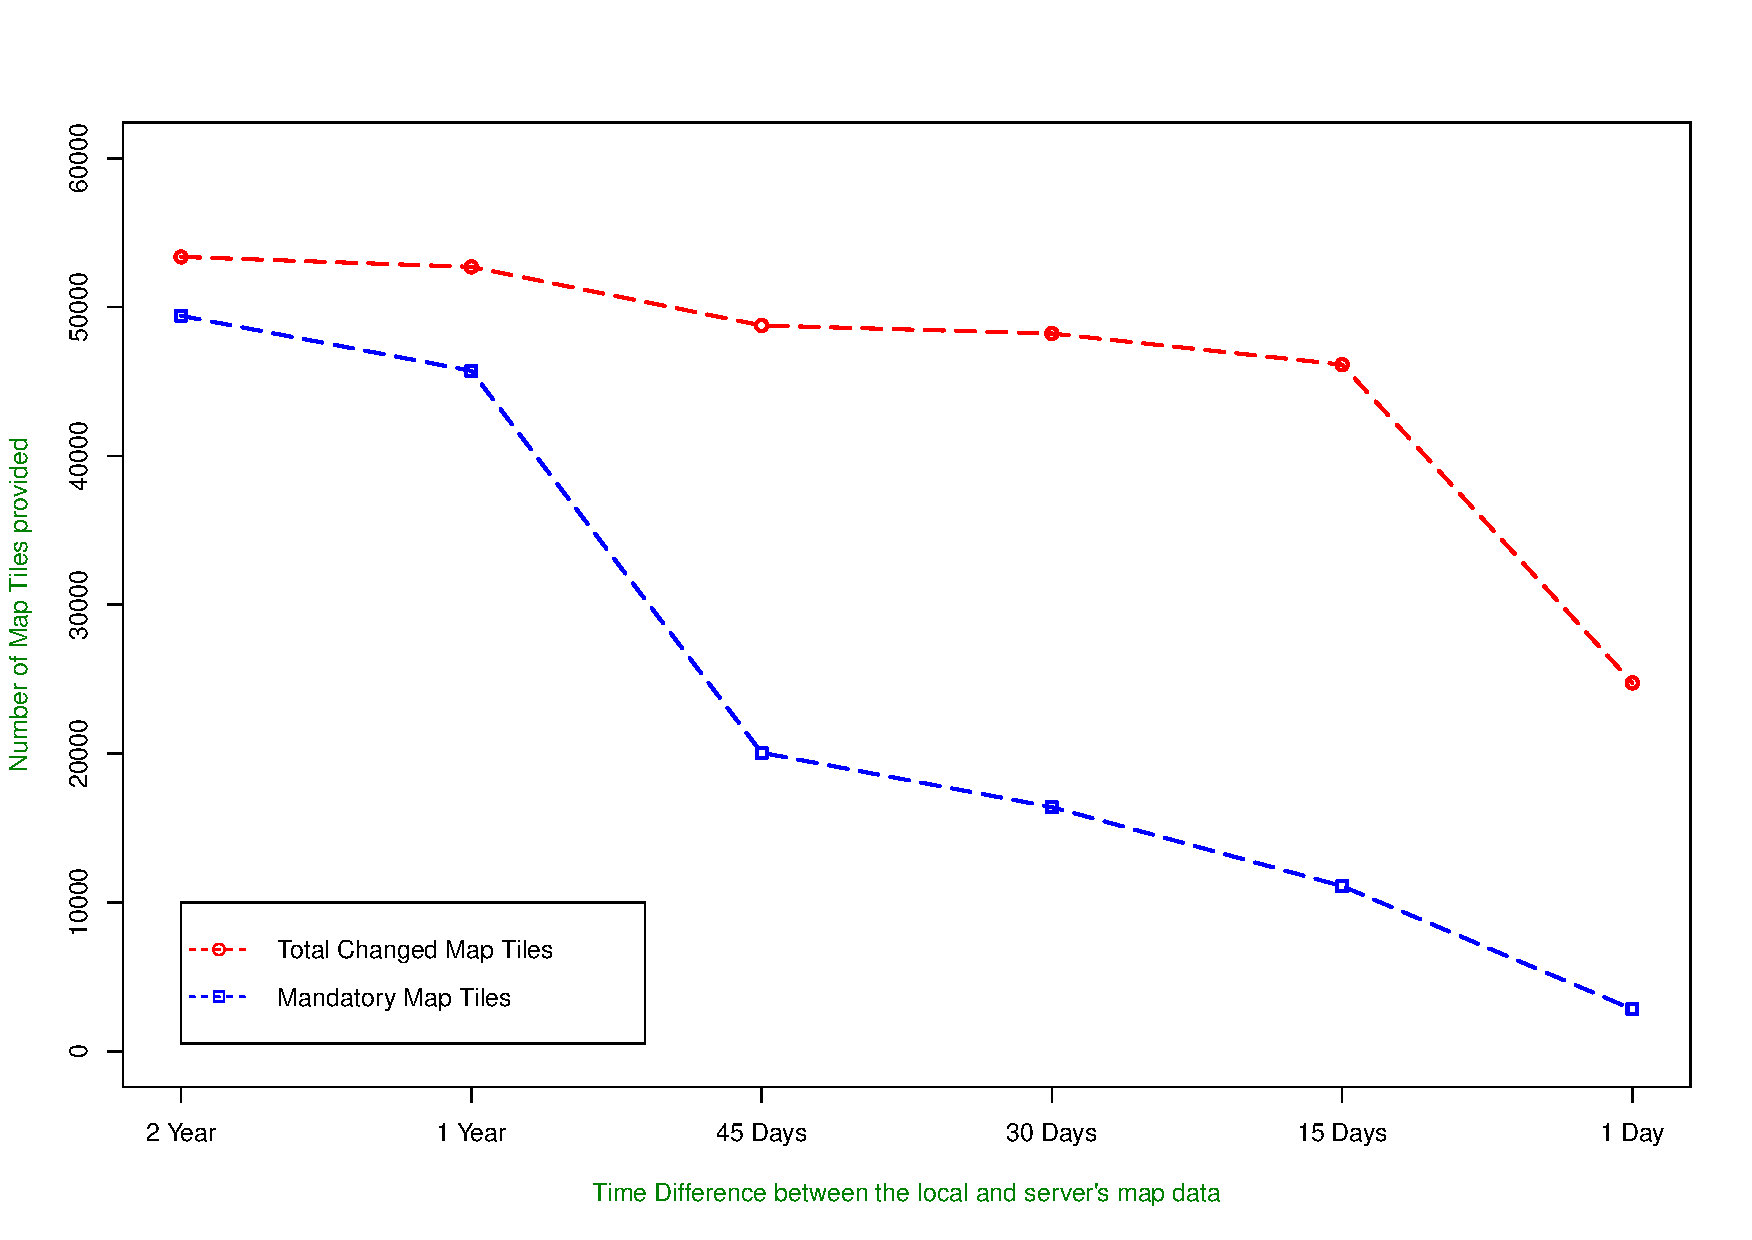
\includegraphics[scale=.6]{Graph1L.pdf}
\caption{Graph showing the total number of map tiles with updates and the mandatory map tiles identified by the Dynamic Map Update Protocol, required for the route calculation over 10,000 individual trips over different time-differences ranging from 2 year to 1 day. For time differences, dates used in comparison with 31-Aug-2016 are as follows 1. 2 Year (1-Jan-2014) 2. 1 Year (1-Jan-2015) 3. 45 Days (16-Jul-2016) 4. 30 Days (1-Aug-2016) 5. 15 Days (16-Aug-2016) and 6. 1 Day (30-Aug-2016)}
\label{fg:scenario1}
\end{figure}


\begin{figure}
\centering
%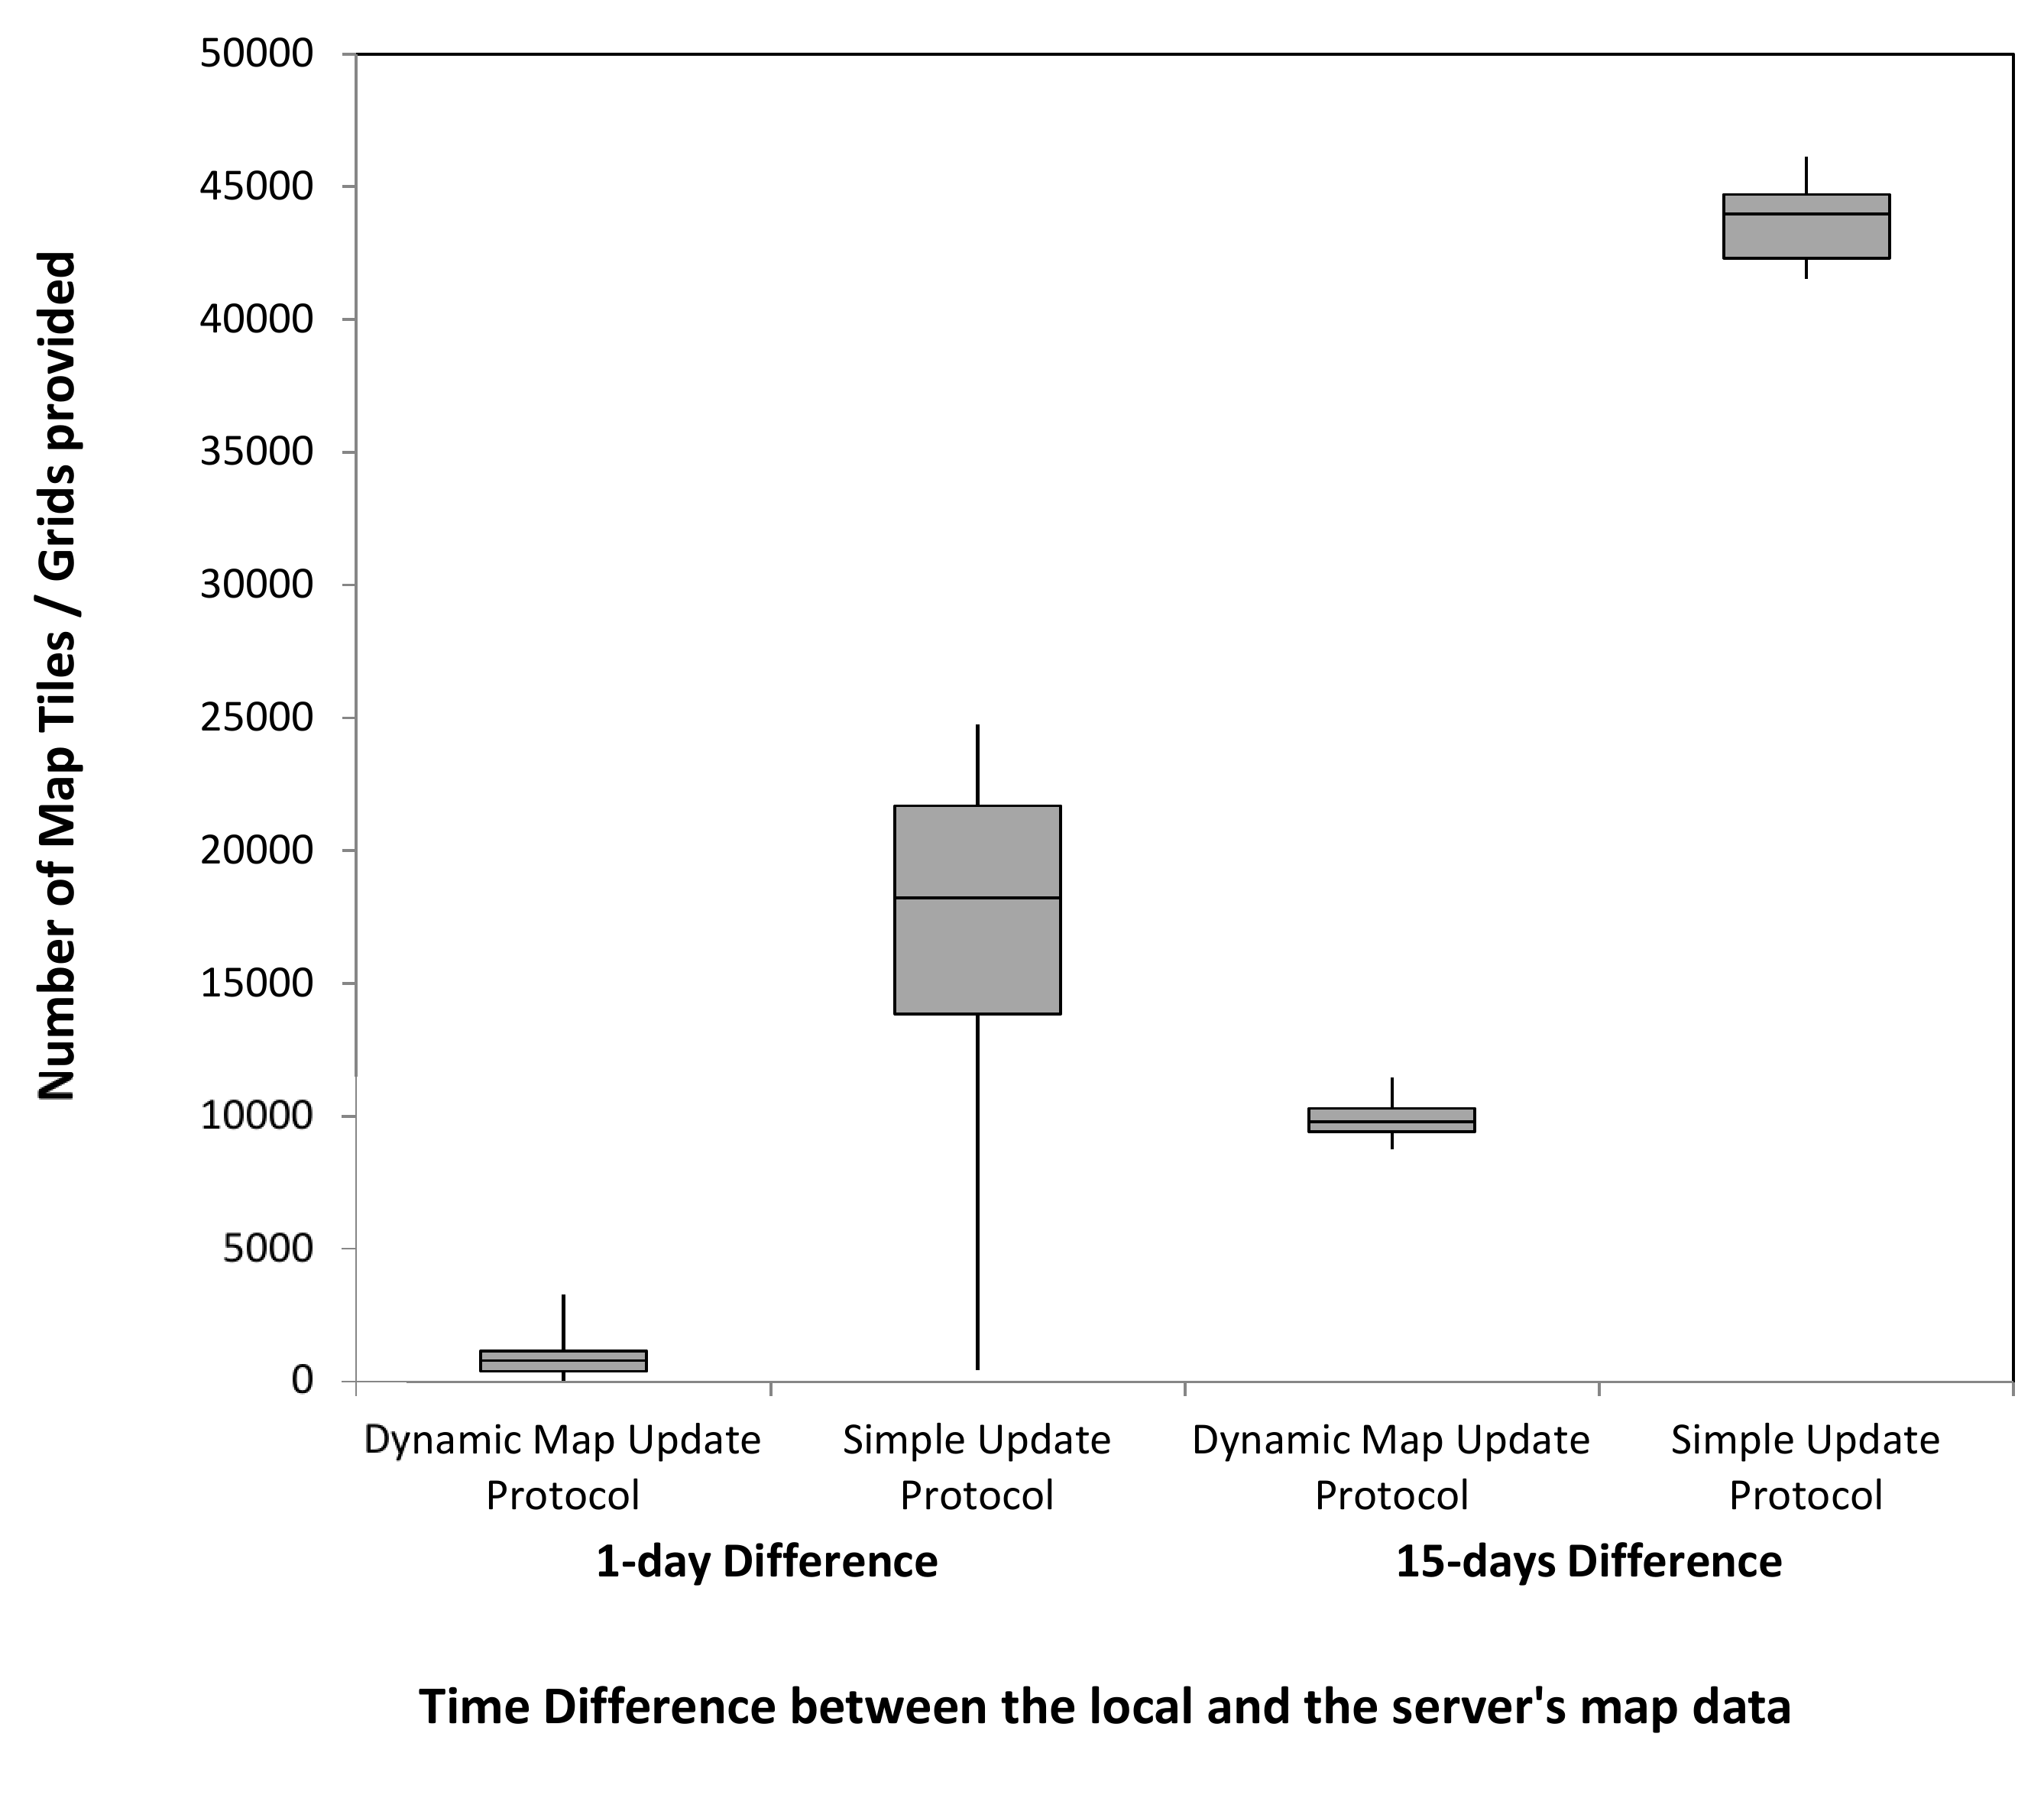
\includegraphics[scale=.25]{scenario1tiles.png}
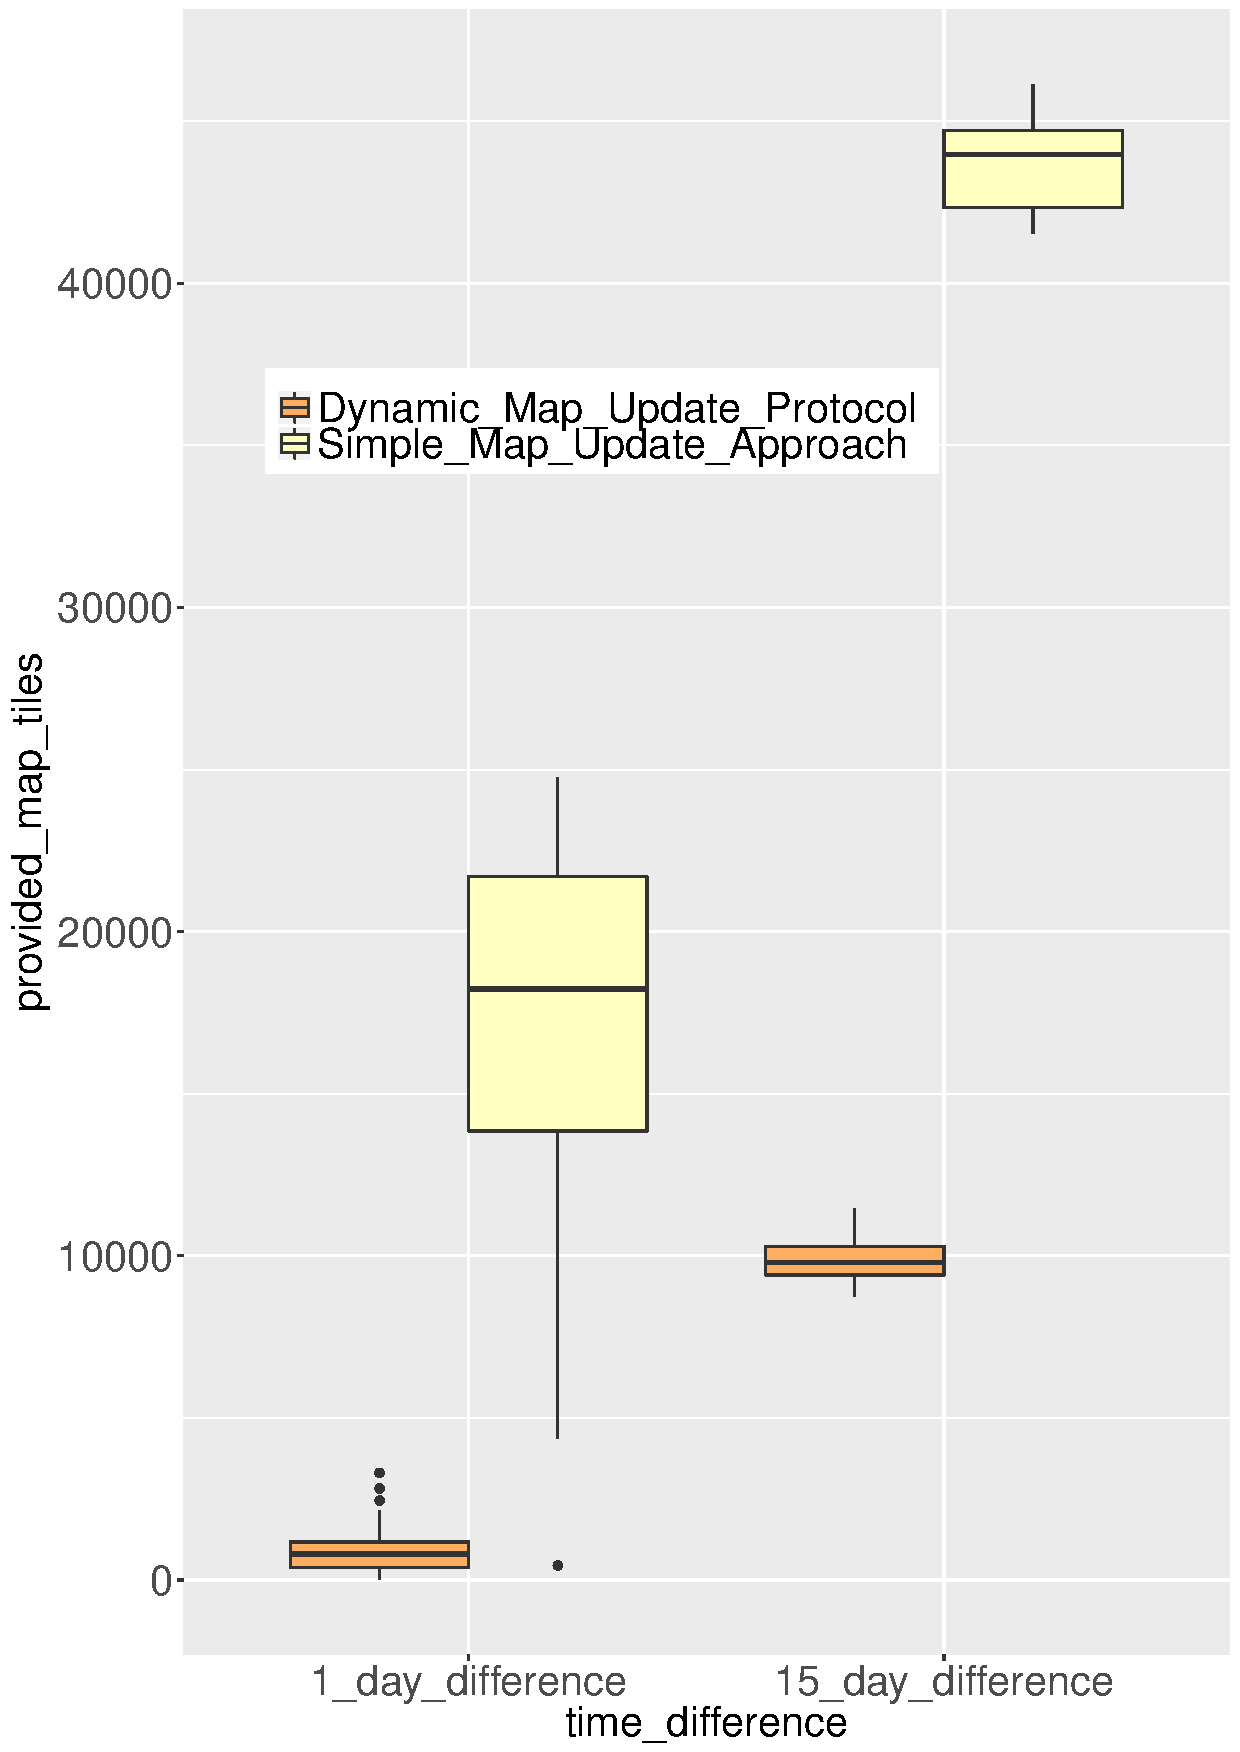
\includegraphics[scale=.7]{MapTiles1dvs15DP.pdf}
\caption{Number of map tiles with updates and total number of mandatory map tiles identified for the server to send update in Scenario 1 for 1-day differences and 15-days differences}
\label{fg:scenario11dv15d}
\end{figure}



We had to verify the results by processing further databases on server side savings, Thus, we evaluated our Scenario 1 (Section \ref{evlscenario1}) for multiple shorter time differences. Using the map databases of the month of August 2016, we evaluated 30 times for 1-day differences and 16 times for 15-days differences. Because OpenStreetMap is a volunteered project, we witnessed variations in the number of changes in the map data for each day. However, our approach still managed to save a significant (94.6\%) amount of map tiles from processing and transmission at the server side. We evaluated scenario 1 using the same set of trips throughout Berlin city. Figure \ref{fg:scenario11dv15d} shows the result of that evaluation. On an average for 1-day difference between the car's and the server's map data, the server had to process and transmit only 929 map tiles in our approach instead of an average of 17273 map tiles. That results in approximate 94.6\% savings. \\

For the 15-days differences evaluation, the amount of map tiles server had to process increased. This is similar to the behavior we saw earlier. On average, the server had to process 9945 map tiles. In the simple approach, the number would be 43732. Our approach resulted in 77.26\% savings. The amount of savings on the server side in terms of map tiles is huge. \\



%However, the number of map tiles fails to provide the correct picture. To present a better picture, we plotted the same graph using the values of the actual map objects. A map object could be considered as one map element which has been added/deleted/updated in the newer version of the map. Figure \ref{fg:scenario11dv15dobject} compares the savings on the server side in terms of   


\subsection{Savings for a highly automated car}
Through evaluation of savings at the server's end, we showed the effectiveness of our approach to save data from being processed and transmitted to the clients on the server side. However, for our approach another important quality criteria is the savings on the autonomous car's side. The savings in terms of cellular data for an autonomous car are directly related to savings in terms of money. The processing costs required on client side are negligible in comparison to cellular data costs. For this, we evaluated our approach for Scenario 2 as described earlier in Section \ref{scenario3}. The evaluation consists of an autonomous car completing 100 connected trips throughout the city while requesting map updates for each trip. The connected trips here mean that the car will start their \textit{n+1}th journey from their previous (\textit{n}th) trips's destination. While doing so, it is expected that the autonomous car will travel along some of the same streets covered in one of its previous trips or at least some of the map tiles it previously traveled through. Because of this, map updates from the previous requests are assumed to be applied at the local map database of the car while requesting an update for the next trip. In the previous scenario (Section \ref{evlscenario1}), all trips were independent of each other. However, in this evaluation the map updates from the previous requests are stored. Additionally after every 10 requests, a snapshot of provided map updates was taken to compare our approach with the simple map update approach. \\

\begin{figure}
%\centering
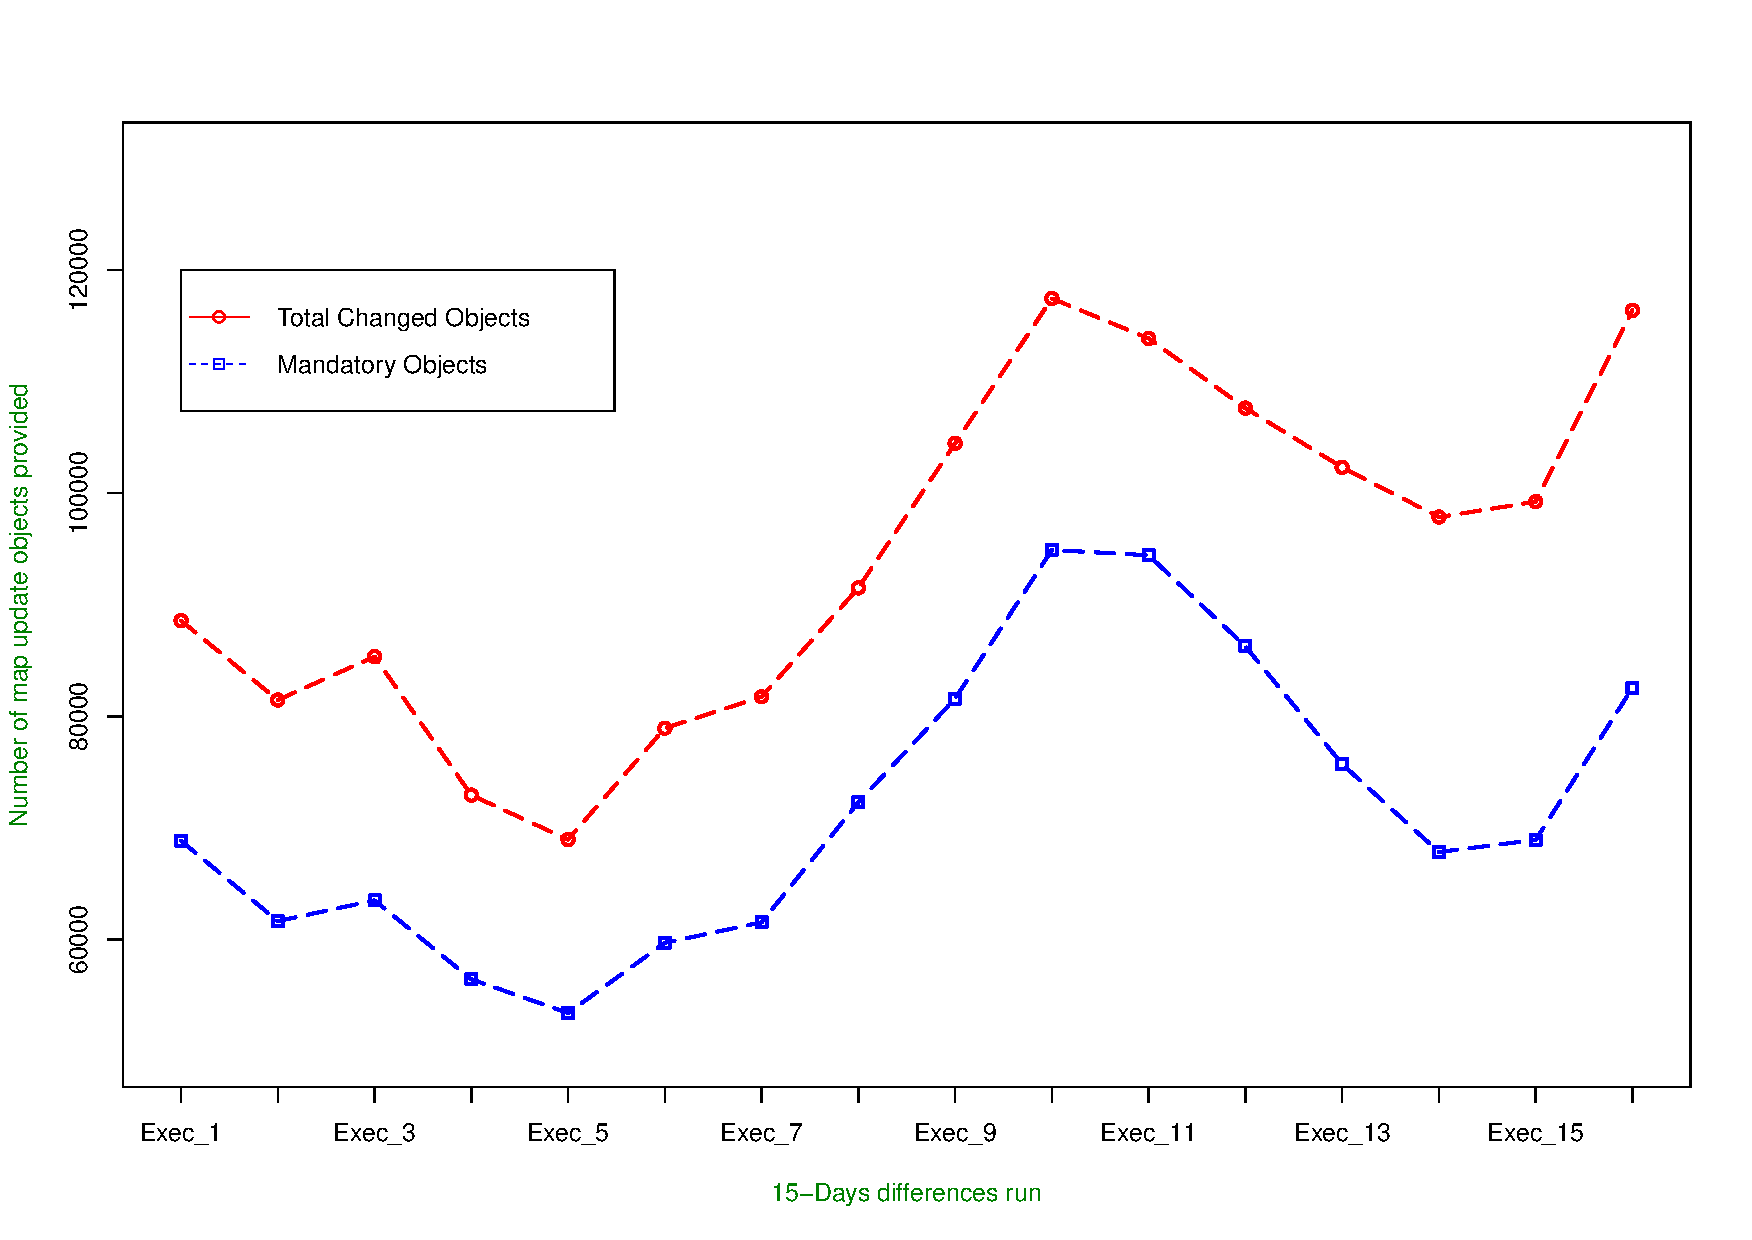
\includegraphics[scale=.6]{15DayDiffL.pdf}
\caption{Graph showing the total number of map objects with changes vs total number of mandatory map objects required with 15-days differences, for 16 runs over the month of August 2016.}
\label{fg:16x15d}
\end{figure}

Figure \ref{fg:16x15d} plots the difference between the number of map objects which are provided by the simple approach along with a comparison to our approach for 15-days difference between the map server and locally available map data. The figure plots 16 such executions which we evaluated for the month of August 2016. The OpenStreetMap (OSM) (Section \ref{osm}) is built through voluntary contribution by members of the OSM community. It is clear from the figure that the number of update objects varies with different executions. However, the required map objects from our approach are always less than the total required update objects in the simple approach. The average saving for those 16 executions was 23.85\%. \\

\begin{figure}
\centering
%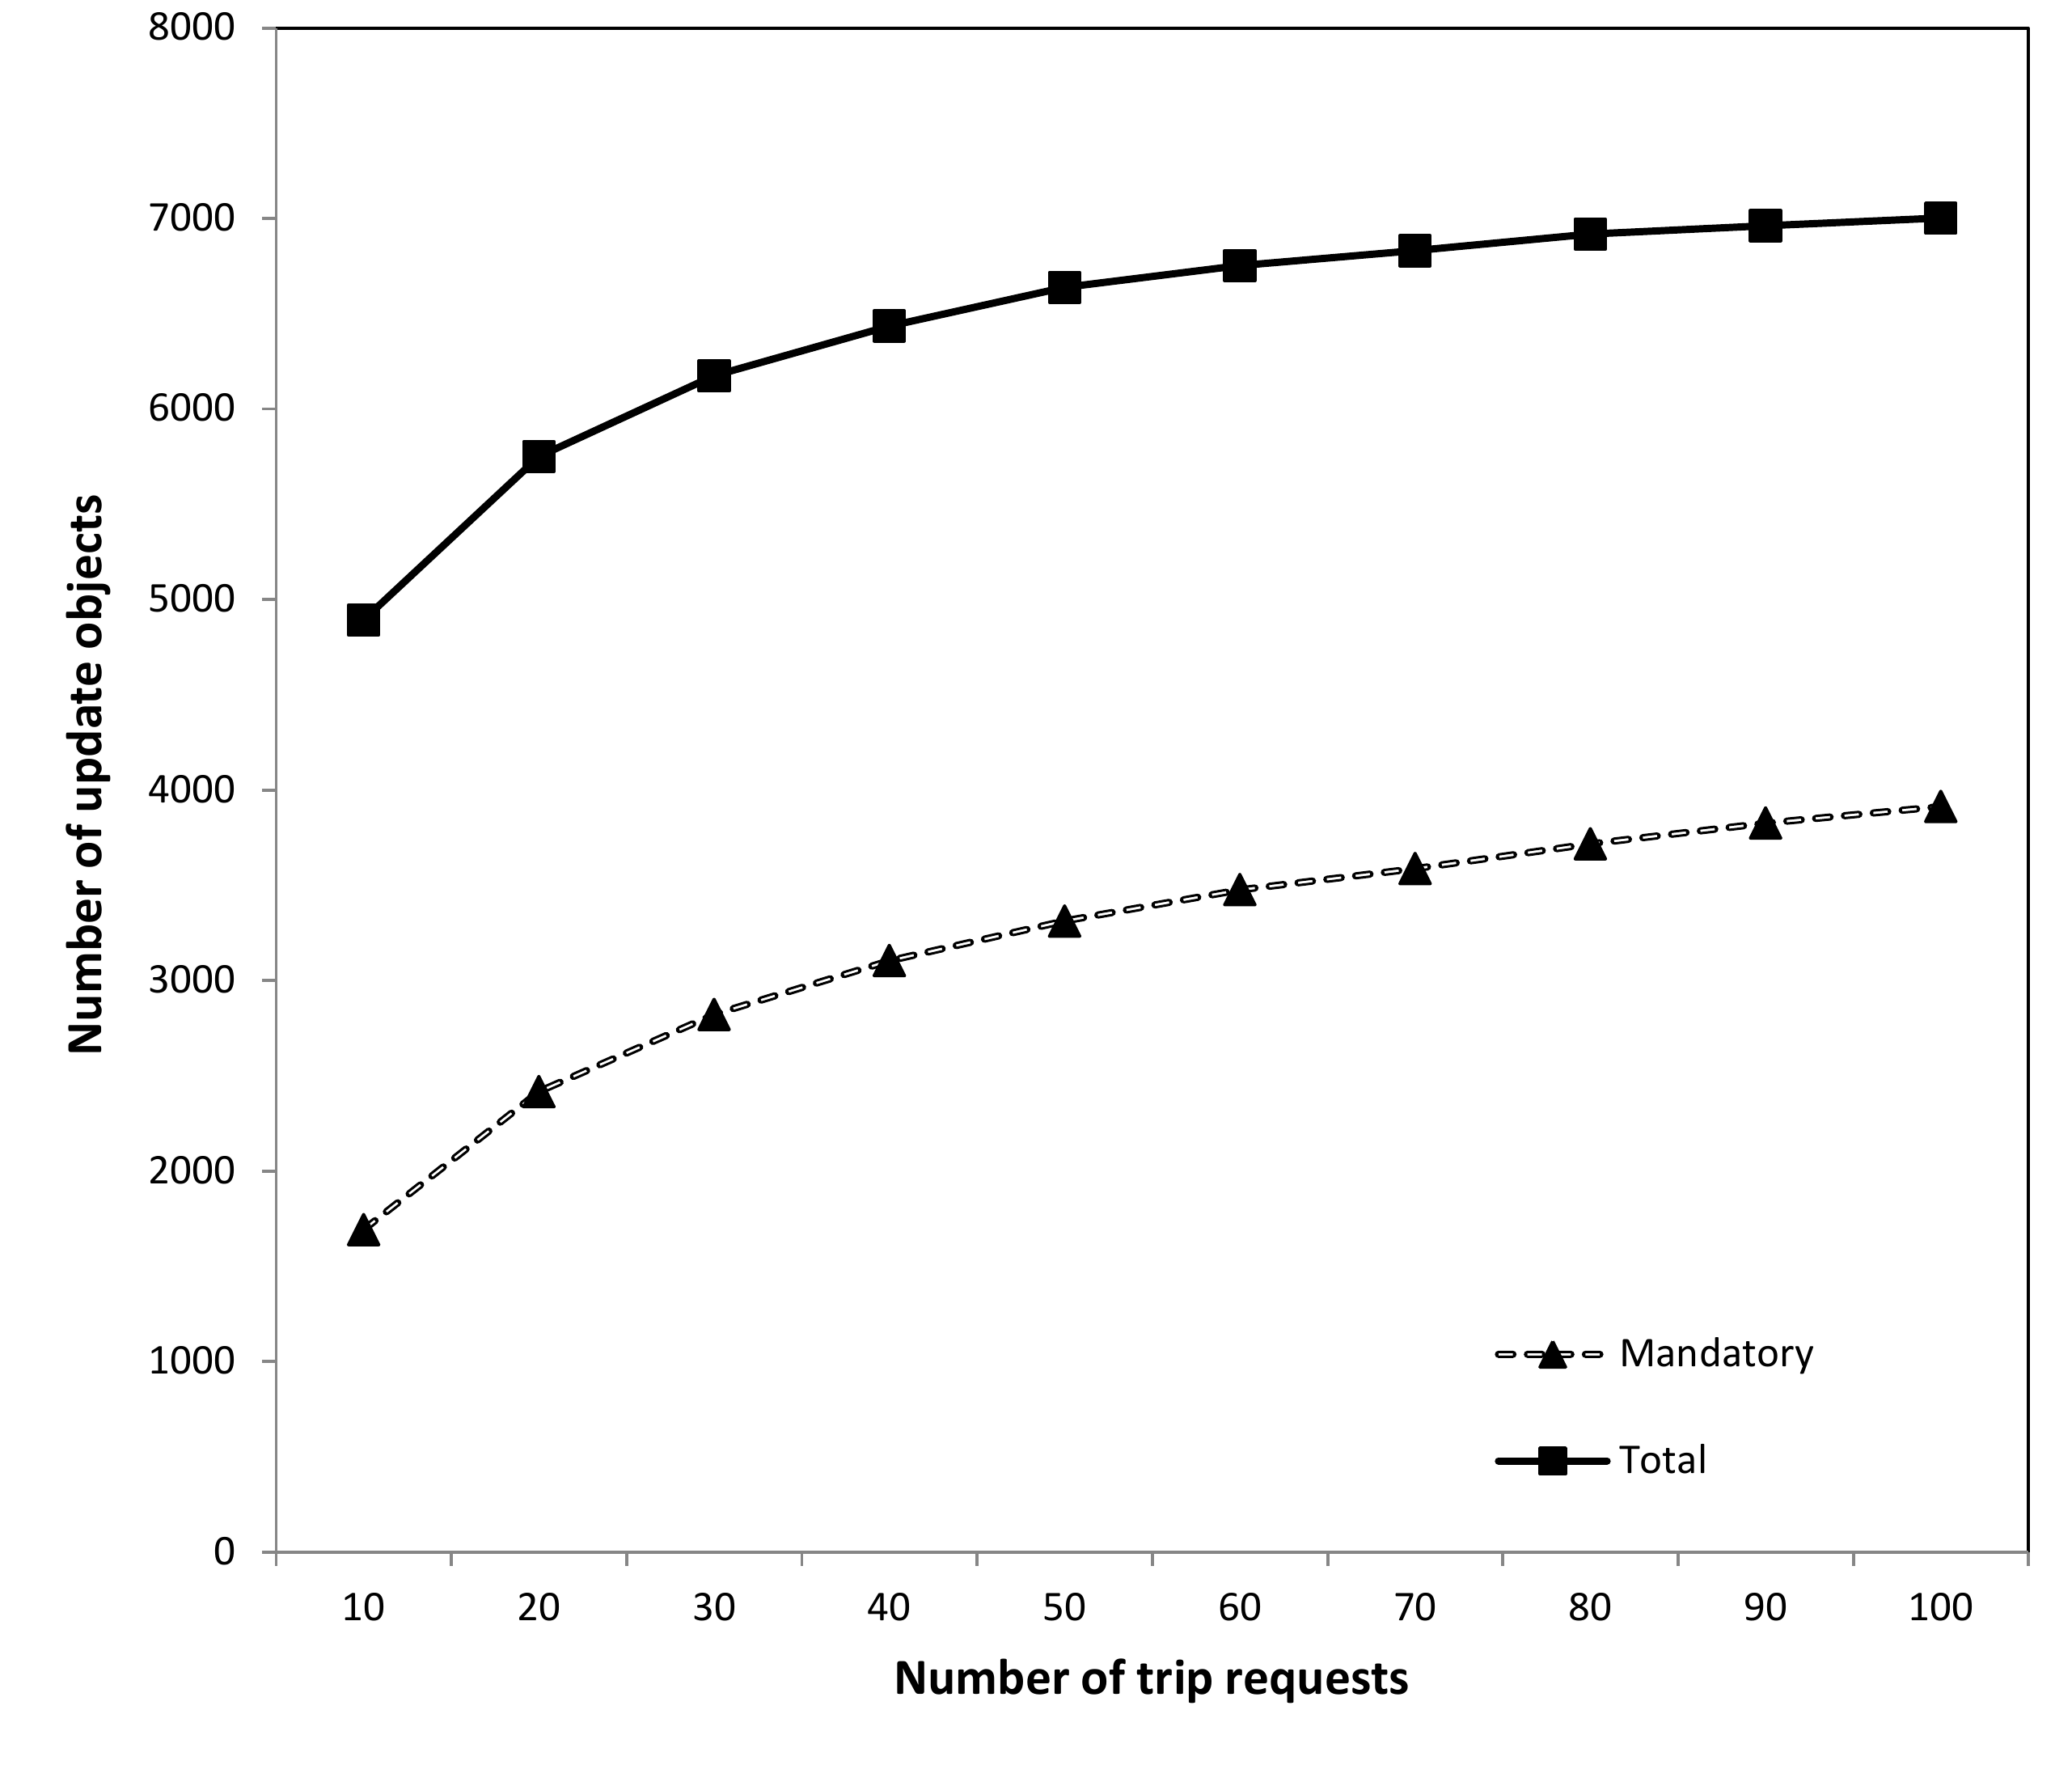
\includegraphics[scale=.25]{1day100x100.png}
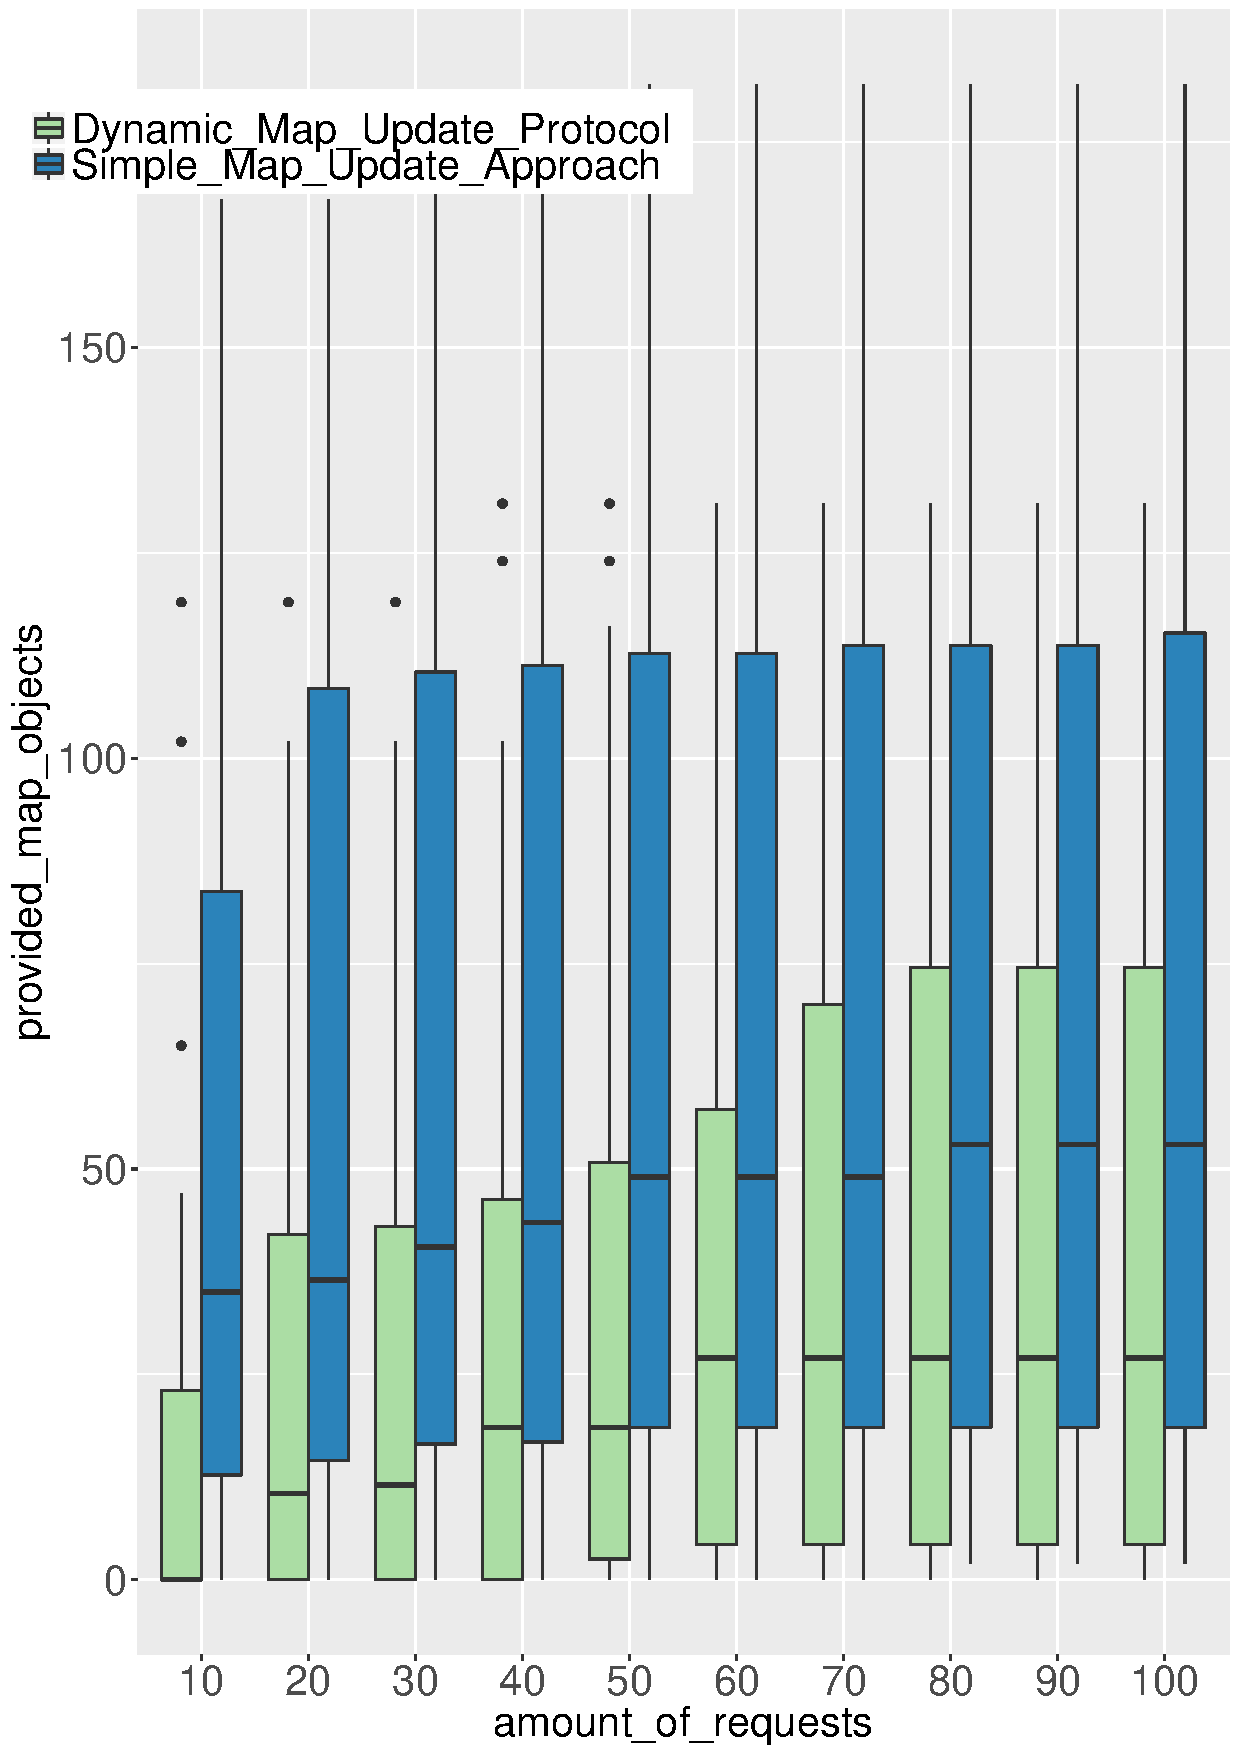
\includegraphics[scale=.7]{Ttest1DayP.pdf}
\caption{Graph showing the difference the between the requested number of update objects for 100 consecutive requests, taken after 10 trips, by 100 different cars over 1-day difference between the local and server's map data.}
\label{fg:ber1d100}
\end{figure}

We previously stated that snapshots were taken after every 10 requests while evaluating the scenario (Section \ref{scenario3}). Figure \ref{fg:ber1d100} compares the amount of map updates provided after every 10 trip requests between our approach and the simple update approach for 1-day differences. It is now clear that our approach saves a significant amount of data while providing only the mandatory map update objects for such trips. We verified this by conducting a t-test on the request patterns for the amount of map updates. Another pattern to notice here is that, the our approach provides a relatively linear request pattern for map updates than the simple map update approach. In this Scenario (see Section \ref{scenario3}), each individual autonomous car is driving 100 different trips. For the given scenario out of the total 7001 map objects requested by the autonomous car in 100 requests, 5751 are requested after the first 20 trip requests. That accounts for approximately 82\% of the total map objects requested. Contrary to this, using our approach the car requests only 62\% of the total map objects in first 20 trip requests. This can lead to higher saving of data as we have considered extreme scenarios of autonomous car doing 100 trips per day. \\

\begin{figure}
\centering
%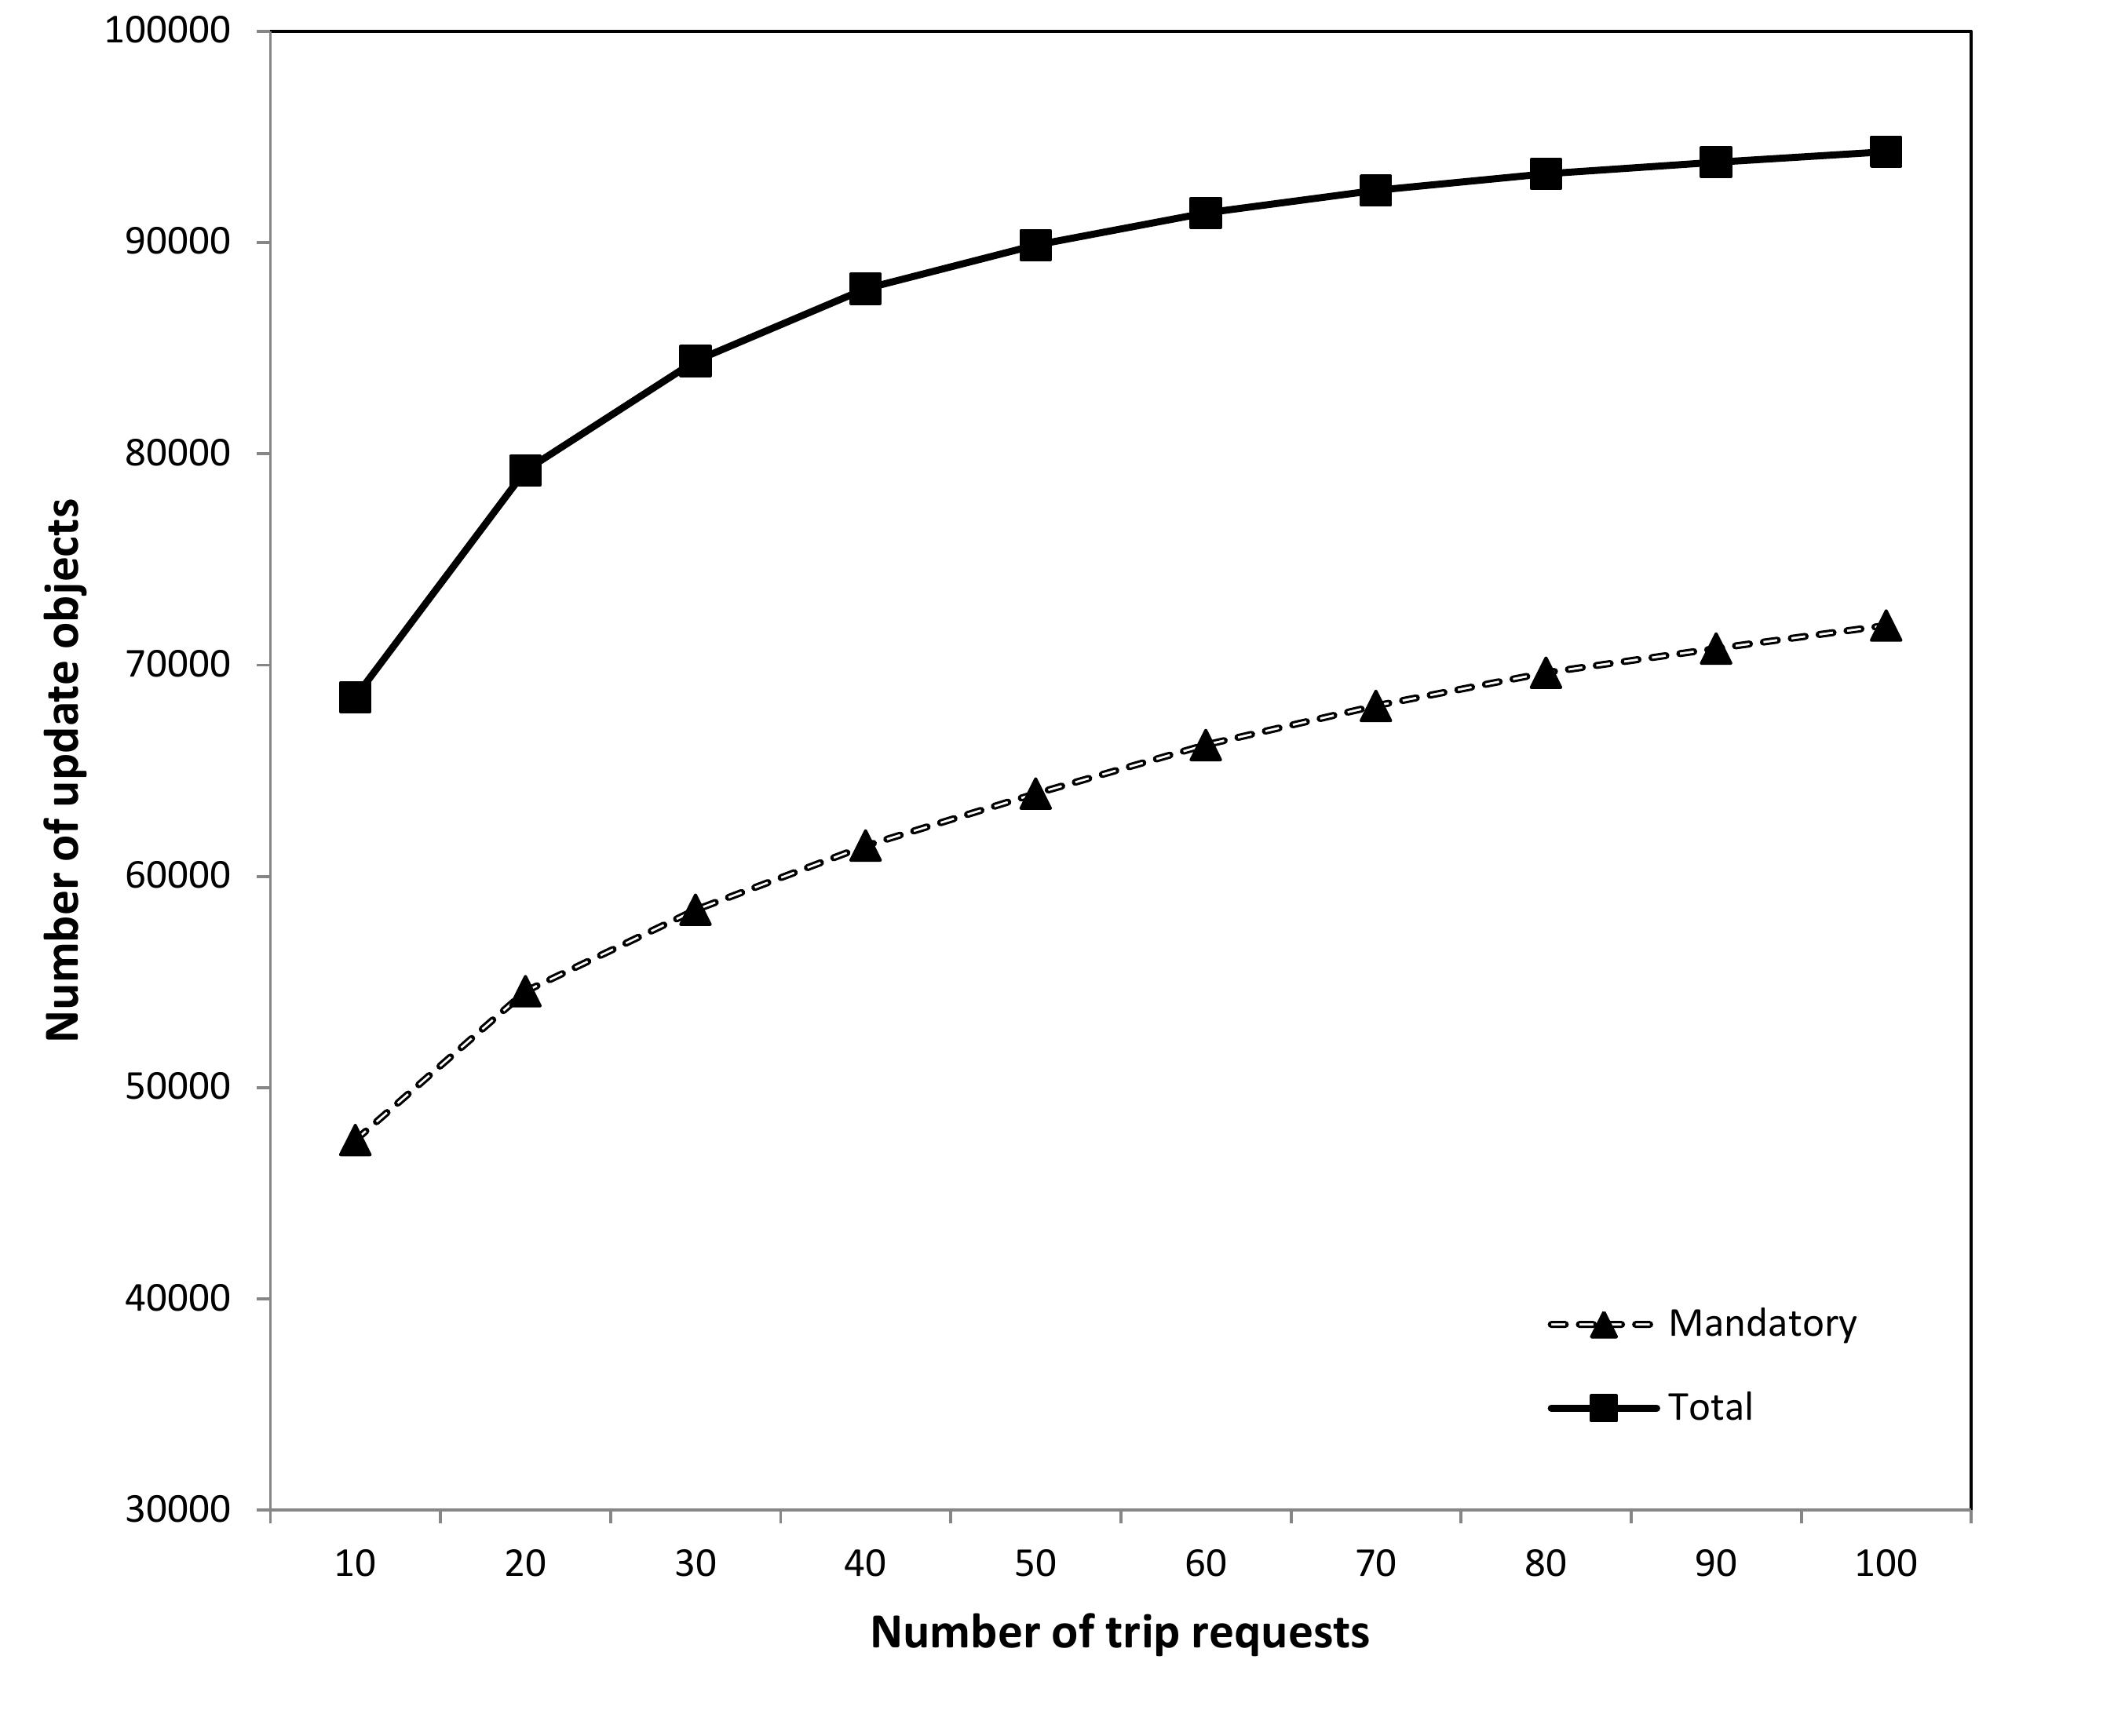
\includegraphics[scale=.25]{15day100x100.png}
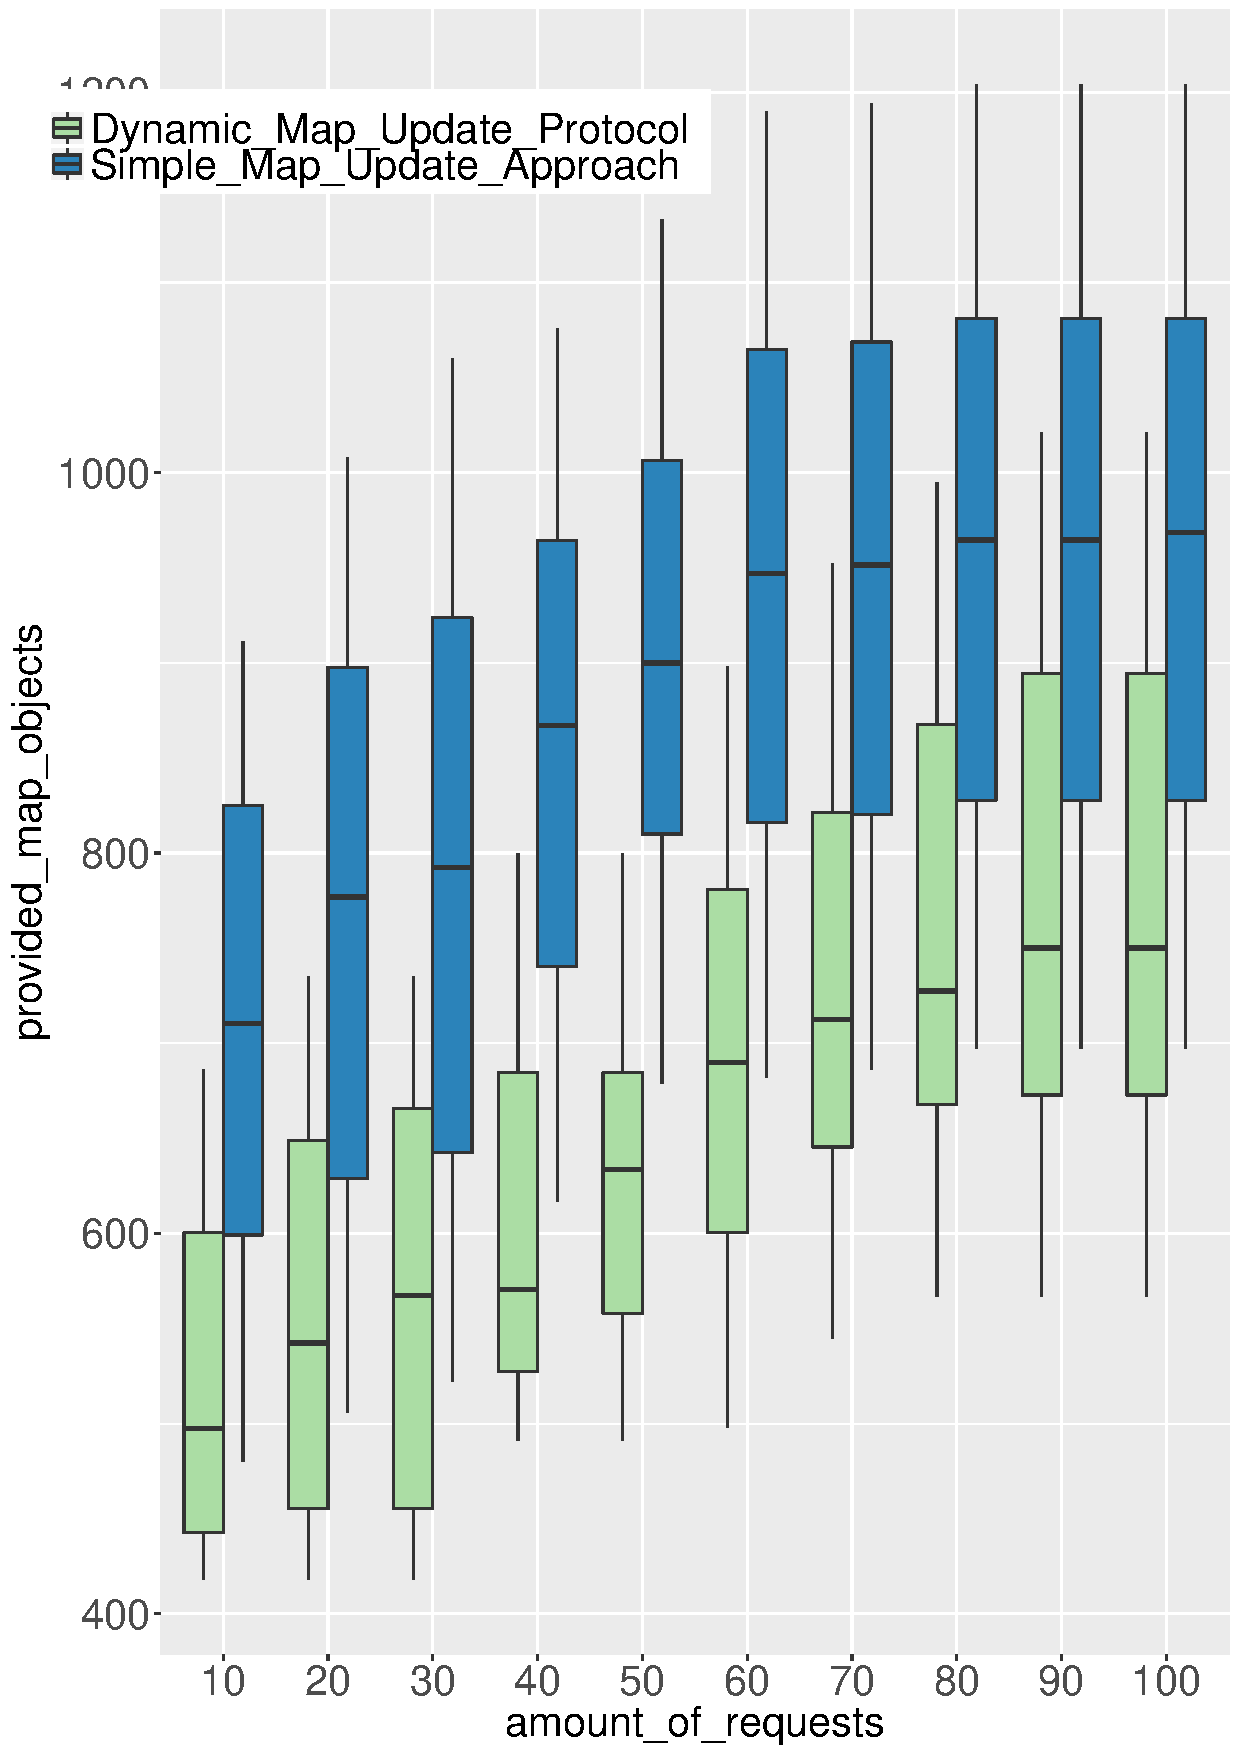
\includegraphics[scale=.7]{TTest15DayP.pdf}
\caption{Graph showing the difference the between the requested number of update objects for 100 consecutive requests, taken after 10 trips, by 100 different cars over 15-days difference between the local and server's map data.}
\label{fg:ber15d100}
\end{figure}

Similarly, Figure \ref{fg:ber15d100} plots the amount of map updates provided after every 10 trip requests for 15-days differences. Similar to earlier observations, we can notice that our approach is relatively linear in terms of providing map update objects to the autonomous car based on the trip requests. After 20 trip requests, the simple update approach provided 84\% of the total map update objects. However, our approach results in significant savings as only 54551 map objects are provided out of total 71859 after first 20 trip request. That amounts to only 59\% of the total map update objects in our approach. We already discussed that the actual savings will be more as our evaluation scenario considers 100 trips per autonomous car. This would mean that on an average each trip has to last only 14 minutes and 24 seconds for continuous 24 hours. This is an extreme situation considering the length of each trip as described in Section \ref{evaluationParameters}.  \\


As clear from the Figure \ref{fg:16x15d}, the amount of map updates varies according to various factors. Additionally, in Figure \ref{fg:ber15d100} and \ref{fg:ber1d100}, we can see some overlap between the amount of map objects provided by Simple Update Protocol and our Dynamic Map Updated Protocol. 
To ensure the statistical significance of the achieved means in our results, we further conducted a paired t-test on the test results. The obtained p-values for the different amount of requests are presented in Table \ref{tablettest} and indicate clearly that we can reject the null hypotheses $H_{0}$: "The two approaches provide the same overhead in terms of update data."
\begin{equation}
H_0: \mu_{dynamicMap} = \mu_{simple}
\end{equation} 
There, we accept the alternative hypothesis  $H_1$: "The Dynamic Map Update Protocol transmits less data than the simple map update approach." 
\begin{equation}
H_1: \mu_{dynamicMap} < \mu_{simple}
\end{equation}
Where $\mu$ is the mean of the number of updated map objects.\\ 


\begin{table*}
\caption{Obtained p-values of the paired t-test for the results of the second test.}
\begin{scriptsize}
\centering
\begin{tabular}
{p{1.5cm}p{1cm}p{1cm}p{1cm}p{1cm}p{1cm}p{1cm}p{1cm}p{1cm}p{1cm}p{1cm}}
number of requests&	10  & 20  & 30  & 40 & 50 & 60 & 70 & 80 & 90 & 100 \\ 
\hline 
1 day time difference & 1.90e-06 & 1.46e-06 & 1.06e-06 & 2.69e-06 & 9.75e-07 & 5.40e-07 & 1.40e-06 & 1.42e-06 & 1.36e-06 & 1.40e-06 \\ 
\hline 
15 days time difference &	8.60e-09 & 3.96e-09& 1.36e-09 &7.14e-11& 1.39e-12 &1.69e-13 &3.43e-11 &2.12e-10 &4.14e-11 &8.03e-11 \\
\end{tabular}
\end{scriptsize}
\label{tablettest}
\end{table*}





The amount of trips we have choosen is quite high to identify saturation of our approach. Completing 100 trips in a day means on average 15 minutes for each of the trips which should be of length greater than 10 kilometers. It is highly expected with reference to \cite{pasaoglu_driving_2012} that only a few autonomous vehicles will come close to this huge amount of trip requests. Therefore, to consider a more reasonable amount of trip requests, we evaluated our approach against another scenario (see Section \ref{10trips}) involving 10 continuous trips for 1000 autonomous cars in the city of Berlin. This evaluation also shows that our evaluation is not affected by the chosen set of trips evaluated for the previous scenario (See Section \ref{scenario3}). We evaluated this scenario with the same time differences of 30 such 1-day differences and 16 of our 15-days differences in the database. Figure \ref{fg:ber10x1000mo} compares the savings in terms of map objects for the aforementioned period. For 1-day differences between the car's and the server's map data, we see an average of 16681 map objects required in our approach in comparison to 48810 by the simple update approach. That accounts for approximately 77\% reduction in the amount of map objects required. Similarly, for the 15-days differences, on average, we required 473742 map objects in our approach. The simple approach required 676129 map objects on an average. Thus, the savings for 15-days differences is approximately 30\%. Due to the relatively large time difference between the map versions of the car and the server, the amount of savings is reduced. 

\begin{figure}
\centering
%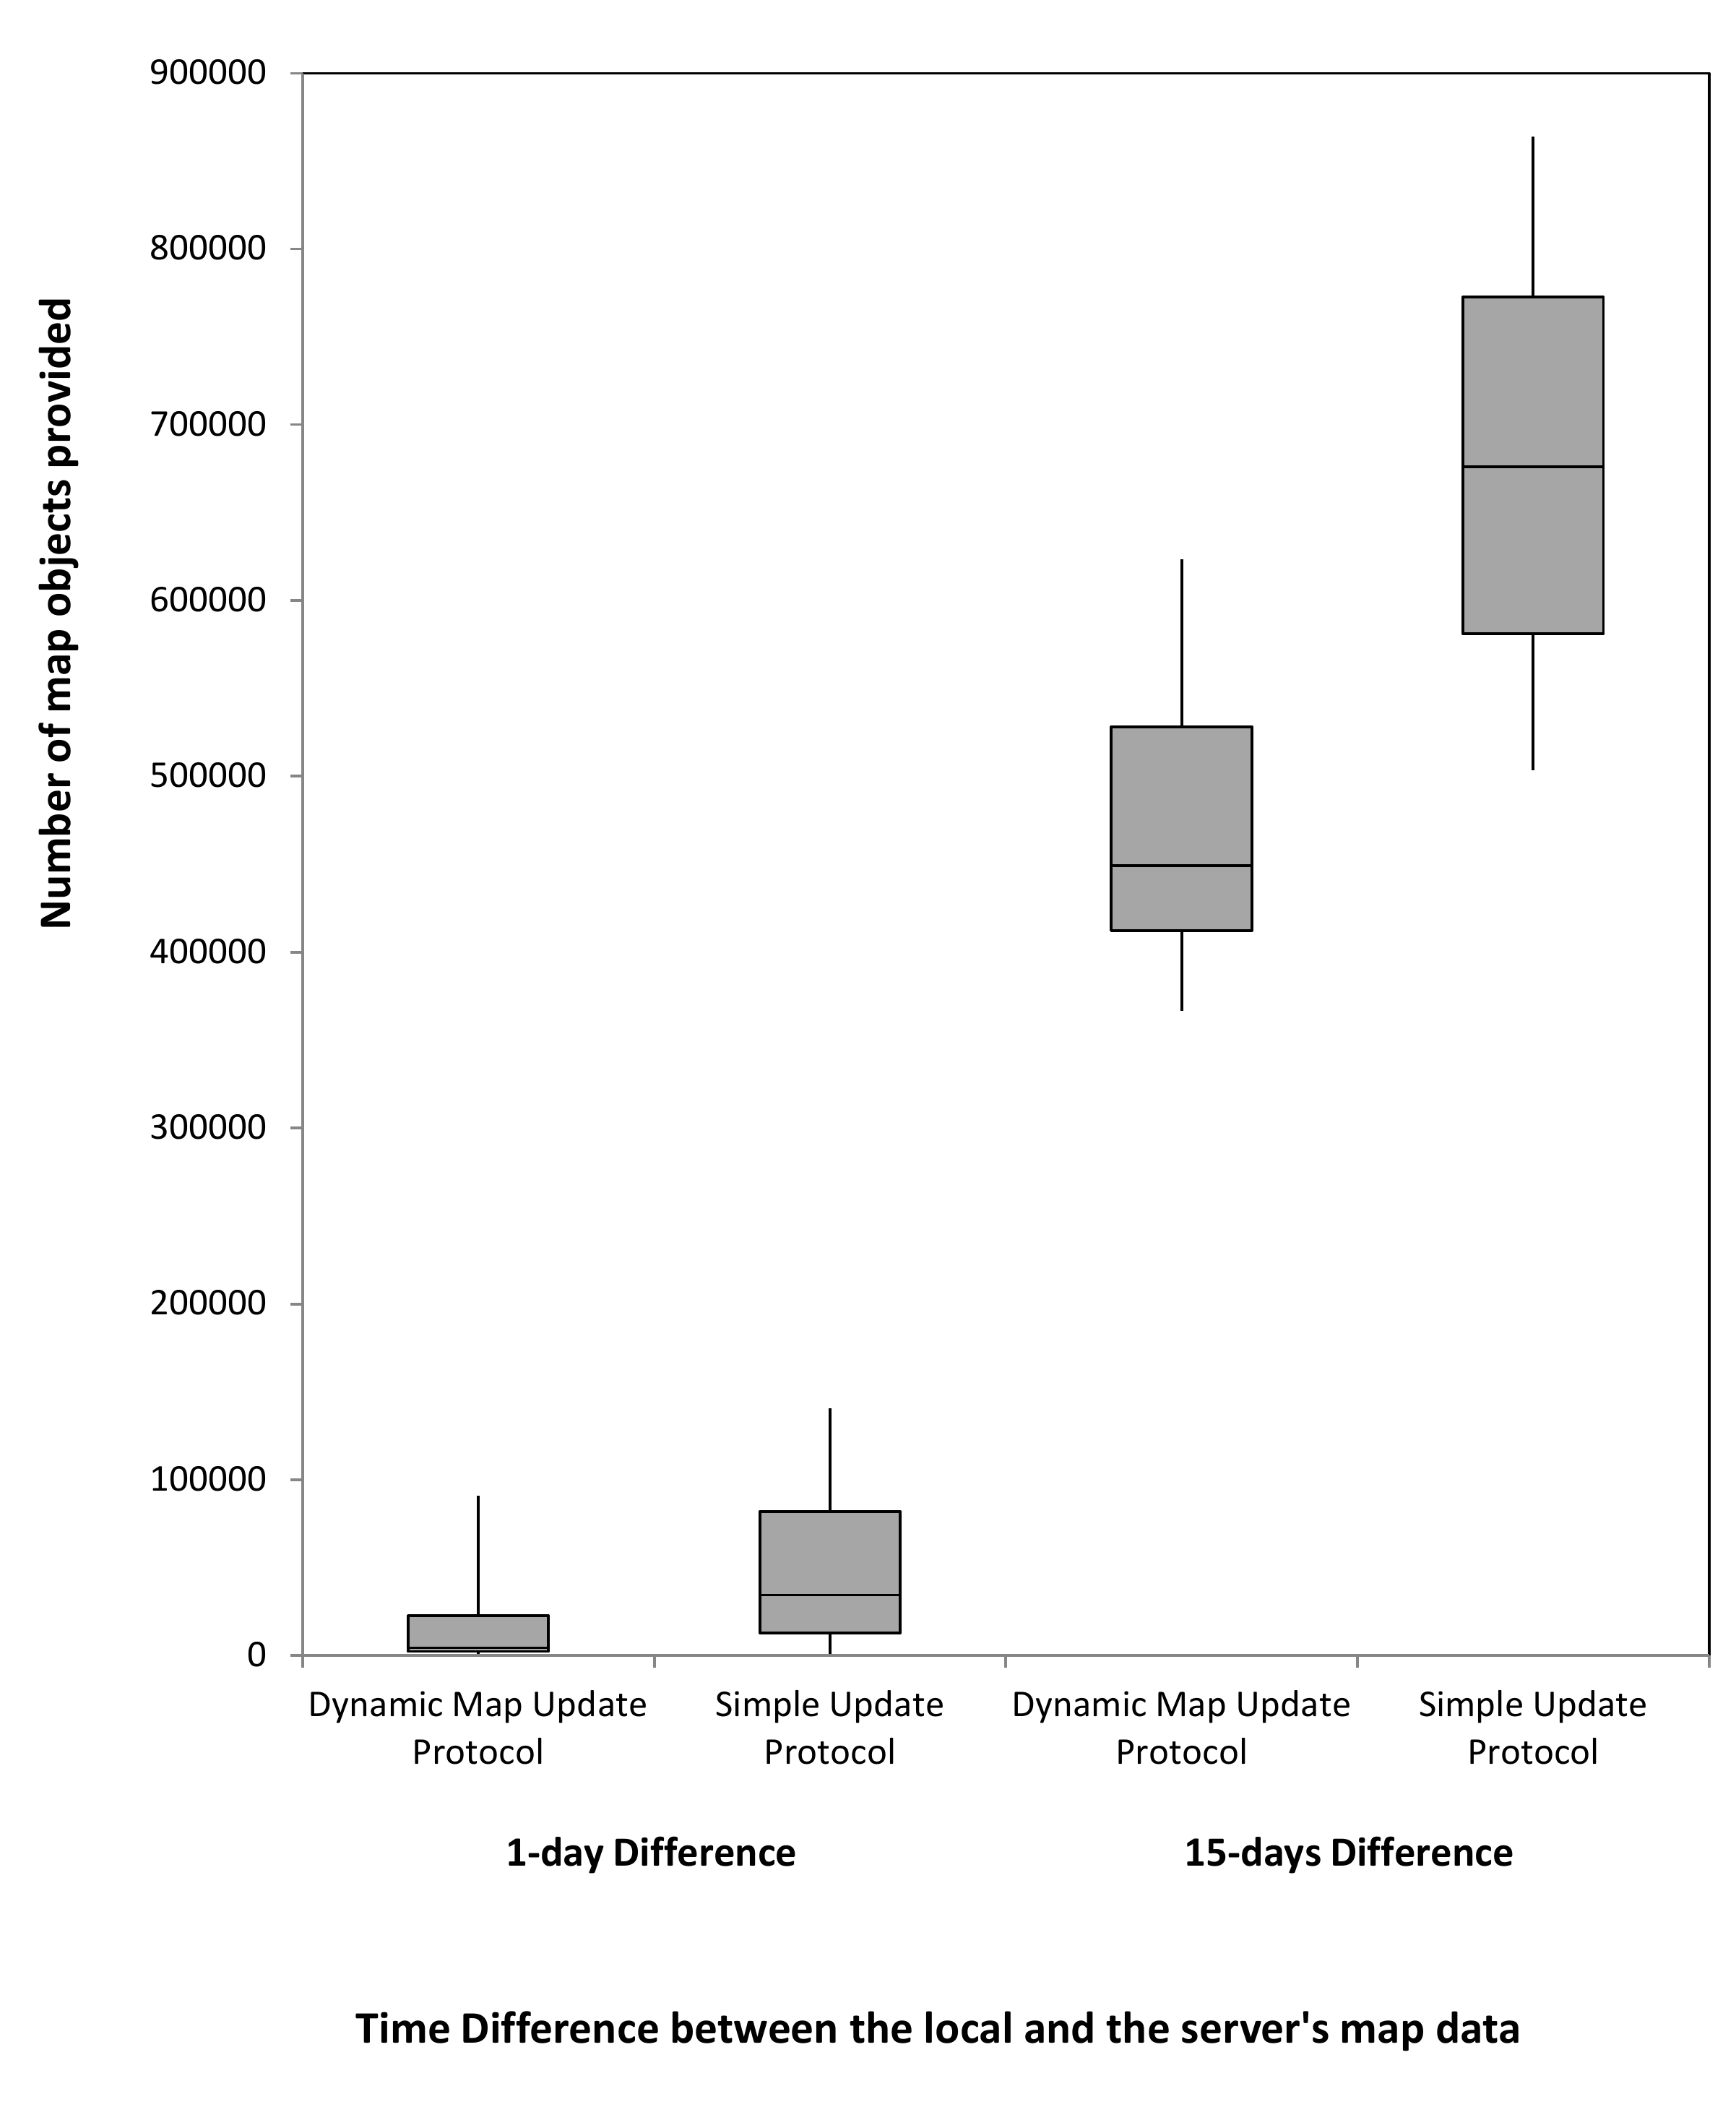
\includegraphics[scale=.25]{10x1000mapobjects.png}
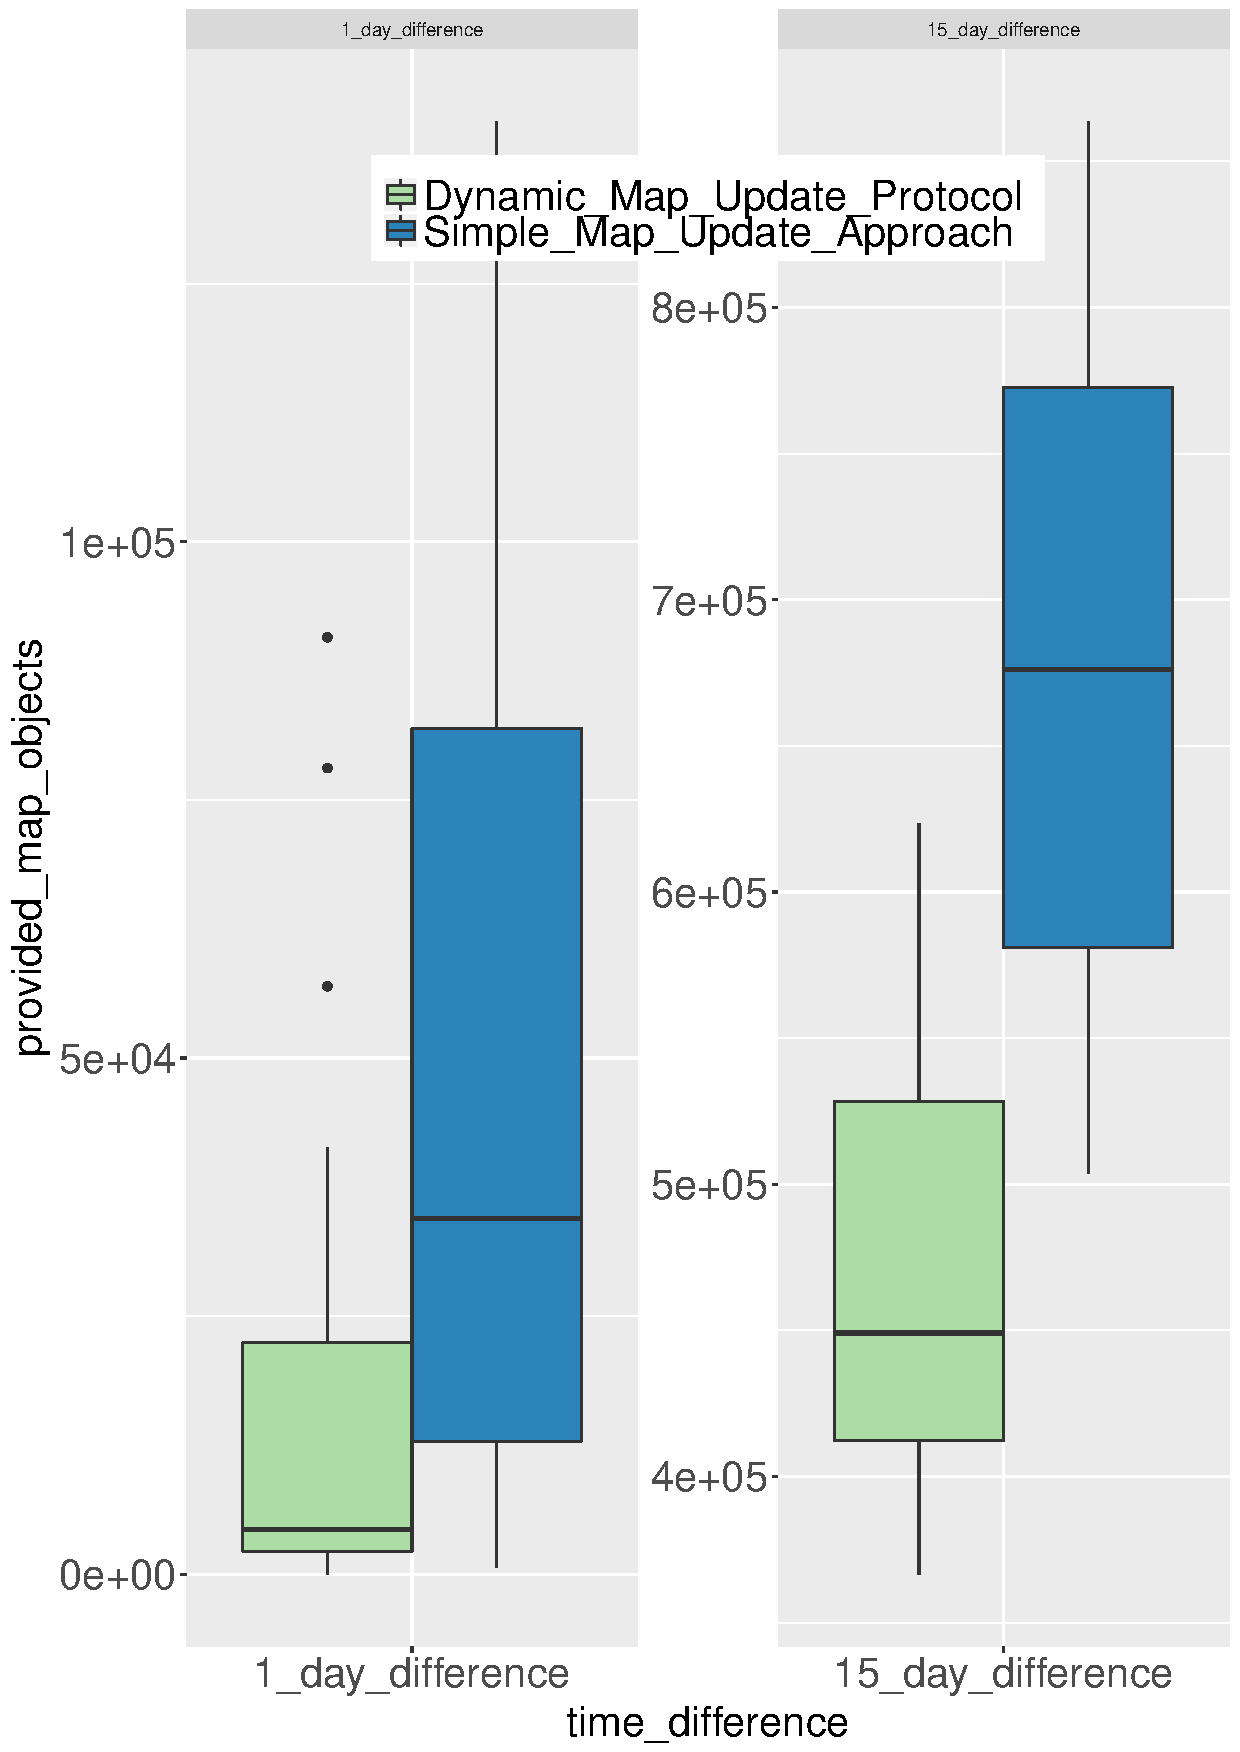
\includegraphics[scale=.7]{MapObjects1dvs15DPLast.pdf}
\caption{Graph showing the difference between the average number of update objects for 10 consecutive requests by 1000 different cars over 1-day difference and 15-days difference between the local and server's map data }
\label{fg:ber10x1000mo}
\end{figure}

  


%\subsection{Key findings}
%The Dynamic Map Update Protocol resulted in a significant amount of savings in terms of map tiles/grids over the simple map update protocol. Through %evaluation we showed that the significant amount of map objects are less than 



\chapter{Conclusion} \label{ch:conclusion}
%\section{Summary}
In this thesis, we presented a novel approach of differential map update to minimize the bandwidth required for autonomous cars to obtain a continuous stream of map updates. The approach has been developed to provide a data efficient scheme to serve contextually relevant high-definition map updates to an autonomous vehicle. The approach calculates the significance of the map data updates for a trip request to classify a particular map update as mandatory or optional resulting in reduced bandwidth usage. The significance of the map updates varies according to the specific requirements of an autonomous vehicle. The processing costs are negligible. We have verified the capabilities of our approach by an extensive evaluation with OpenStreetMap data of the German city of Berlin. The achieved results clearly indicate a significant amount of data savings and reduction in processing time for map updates for autonomous vehicles using our approach over the existing solutions.    
\section{Outlook}
With the adoption of autonomous driving cars on a large scale, many research problems will arise. The usage of a high-definition map as a sensory input for autonomous cars is likely to gain more momentum in the future. An updated map will help in ensuring a smoother and safer experience in autonomous vehicles. It is plausible that with a large fleet of autonomous cars in use, the importance of delivering efficient map updates will increase. Although, this thesis answers one aspect of such research problem, further work is required in this area to answer the multitude of related research problems. While the scope of this thesis provided an approach to use contextual information to reduce the map update sizes, many related extensions need to be researched to extend the scope of this work further. 
\subsection{Breadth-first approach} \label{futurebfs}
In Section \ref{gridsizeclassification}, we stated that grid size plays an important role in reducing the amount of updates required in our approach. Instead of marking map tiles/grids as mandatory, we briefly tested our approach to mark linked road objects which have changed between versions, through a breadth-first search approach as mandatory. The search would terminate at a road object which has not changed between two different versions of the map. We believe that, by using this approach further reduction in the data transmission could be achieved. During our tests, we found out that in a heavily updated region like Berlin, often tracing road objects in a breadth-first approach resulted in linking to a main/important road. This resulted in a sprawling list of never ending road objects which had changed in the newer version of the map. Thus, more investigation is needed to devise and evaluate such an approach possibly by limiting the list of sprawling edges at the boundary of a map tile/grid.
\subsection{Efficient Delivery of Map Updates}
We have devised a novel approach to minimize the transmission of map updates by identifying whether they are relevant or not to the current trip. However, our approach does not dictate any approach about efficient delivery of such map updates. \citet{movenet}'s work on MoVeNet approach provides an efficient strategy to handle hand-offs and transmission in a moving object such as an autonomous car. We believe that MoVeNet's approach can be combined with our approach to identify efficient transmission points/locations for mandatory map update transmission. Also, such work could be used to identify an area without network coverage to efficiently plan future mandatory map updates and even the optional map updates depending on the cellular bandwidth cost.



\subsection{Ad-hoc Map Transfer Between Vehicles}
In this thesis, we have identified contextually relevant map tiles/grids updates for an autonomous car. However, the remaining map tiles/grids with changes are marked optional. The delivery of optional map tiles/grids is deferred until it becomes relevant to the autonomous vehicle. It is quite possible that an optional map tile/grid becomes relevant in future. Therefore, it would be beneficial to research alternative approaches to get those optional map updates. Research in the area of Vehicle to Vehicle communications is gaining traction as more connected cars are becoming available. The recent work of \citet{probsense} on ProbSense.KOM investigates such methods of sharing data among vehicles. Combining the work of this thesis and ProbSense.KOM, a model could be evaluated for further reducing the bandwidth required for the map updates.





%*****************************************
%*****************************************
%*****************************************
%*****************************************
%*****************************************
